% master_thesis.tex
% -------------------------------------------------------------------------
%   Modern Minimalist Master Thesis Template - Robotics (SINDy)
% -------------------------------------------------------------------------
\documentclass[
    11pt,               % Standard font size
    a4paper,            % Paper size
    twoside,            % Print on one side (change to 'twoside' for binding)
    numbers=noenddot,   % Removes end dots in numbering (e.g. 1.1 not 1.1.)
    parskip=half,       % Adds space between paragraphs (modern look)
    listof=totoc,       % Adds Lists of Figures/Tables to TOC
    bibliography=totoc  % Adds Bibliography to TOC
]{scrreprt}

% --- Essential Packages ---
\usepackage{fontspec}       % For XeLaTeX font management
\usepackage[english]{babel}
\usepackage{microtype}      % Improves character kerning (essential for 'classy' look)
\usepackage[left=25mm, right=25mm, top=20mm, bottom=25mm]{geometry} % Margins: L25mm R25mm T20mm B25mm

% --- Mathematics & Robotics Specifics (Load BEFORE fonts for compatibility) ---
\usepackage{amsmath}
\usepackage{mathtools}
\usepackage{amssymb}
\usepackage{siunitx}        % Correct unit formatting (e.g. \SI{5}{\meter\per\second})

% --- Fonts (Optimized for XeLaTeX) ---
\setmainfont{Latin Modern Roman}[
    Ligatures=TeX
]
\setsansfont{Latin Modern Sans}[
    Scale=0.9,
    Ligatures=TeX
]
\setmonofont{Latin Modern Mono}[
    Scale=0.9
]

% --- Math Font ---

% --- Japanese Font Support ---
\usepackage{xeCJK}
\setCJKmainfont{IPAexMincho} % For CJK characters
\setCJKsansfont{IPAexGothic} % for \sffamily

\usepackage{scrhack} % listing issue
\usepackage{csquotes} % babel quote
\usepackage{siunitx}        % Correct unit formatting (e.g. \SI{5}{\meter\per\second})

% --- Graphics & Tables ---
\usepackage{graphicx}       % For including images
\usepackage{booktabs}       % Professional tables (no vertical lines)
\usepackage{float}          % Better float placement
\usepackage{subcaption}     % For sub-figures (a) (b)

% --- Algorithms & Code ---
\usepackage[ruled,vlined]{algorithm2e} % For pseudocode
\usepackage{listings}       % For Python/Matlab code
\usepackage{xcolor}

% --- Header & Footer Styling (Clean/Minimalist) ---
\usepackage[automark,headsepline]{scrlayer-scrpage}
\clearpairofpagestyles
\ihead{\headmark}
\cfoot*{\pagemark}  % * makes it apply to both plain and scrheadings styles
\pagestyle{scrheadings}

% --- Hyperlinks (Must be loaded last) ---
\usepackage[colorlinks=true, linkcolor=black, citecolor=blue, urlcolor=blue]{hyperref}

% --- Bibliography ---
\usepackage[style=ieee, backend=biber]{biblatex}
\addbibresource{references.bib}

% --- Tikz ---
\usepackage{tikz}
\usepackage{etoolbox}
\usetikzlibrary{positioning,matrix,backgrounds,calc,fit}


\pgfdeclarelayer{background}
\pgfdeclarelayer{foreground}
\pgfsetlayers{background,main,foreground}

\definecolor{sindynullgray}{RGB}{200,200,200}
\definecolor{sindyforces}{RGB}{196,78,82}
\definecolor{sindynewton}{RGB}{85,168,104}
\definecolor{sindylagrange}{RGB}{129,114,179}

\newcommand{\lb}{[}
\newcommand{\rb}{]}

% Define the sindy component as a node style
\tikzset{
    sindy label/.style={font=\tiny, text=black,minimum height=0pt},
    sindy component text/.style={
        rectangle,
        minimum width=10pt,
        minimum height=1.5cm,
        rounded corners=5pt,
        fill=none,
        draw=none,
        inner sep=0pt,
        outer sep=1pt,
        align=center,
    },
    with label/.style={label={[sindy label]above:#1}},
    deactivated opacity/.style={opacity=0.3},
    full opacity/.style={opacity=1.0},
    sindy solution/.style={
        rectangle,
        minimum width=6pt,
        minimum height=6pt,
        rounded corners=3pt,
        fill=sindynullgray,
        draw=none,
        inner sep=0pt,
        outer sep=0pt,
        align=center,
        opacity=0.3,
    },
    sindy component/.style={
        rectangle,
        minimum width=6pt,
        minimum height=10pt,
        rounded corners=3pt,
        fill=sindynullgray,
        draw=none,
        inner sep=0pt,
        outer sep=1pt,
        align=center,
        opacity=0.3,
    },
}

\tikzset{
    % Le style pour la "patate" : notre système physique réel
    system/.style={
        fill=gray!30, 
        draw=black, 
        thick,
        opacity=0.8
    },
    % Le style pour les fonctions candidates du catalogue
    catalog_function/.style={
        draw=blue!80, 
        fill=blue!20, 
        circle, 
        opacity=0.6,
        line width=1pt
    }
}

\definecolor{sindypreknowledge}{RGB}{196,78,82}
\definecolor{sindystandard}{RGB}{85,168,104}
\definecolor{sindysolutionexplicit}{RGB}{129,114,179}
\definecolor{sindysolutionimplicit}{RGB}{204,185,116}

% --- Custom Commands for SINDy ---
\newcommand{\TODO}[1]{\textcolor{red}{\textbf{TODO: #1}}}

\newcommand{\thesisunderline}[1]{\noindent\vbox{#1\par\vspace{-2pt}\hrule height 0.4pt width \hsize}}

% -------------------------------------------------------------------------
%   DOCUMENT BEGINS
% -------------------------------------------------------------------------
\begin{document}

% --- Cover Page (Japanese/English Format) ---
\begin{titlepage}
    \centering
    \vspace*{0.75cm}
    
    {\fontsize{28pt}{30pt}\selectfont 修士学位論文 \par}
    \vspace{0.2cm}
    {\fontsize{28pt}{30pt}\selectfont Master's Thesis \par}
    
    \vspace{1.5cm}
    
    {\fontsize{16pt}{18pt}\selectfont 論文題目 \par}
    \vspace{0.2cm}
    {\fontsize{14pt}{16pt}\selectfont Thesis Title \par}
    
    \vspace{1.5cm}
    
    {
    \fontsize{16pt}{18pt}\selectfont
    \thesisunderline{ \textbf{Discovering Nonlinear Dynamics by Simultaneous}}\par
    \thesisunderline{ \textbf{Lagrangian and Newtonian Identification for}}\par
    \thesisunderline{ \textbf{Implicit and Explicit Sparse Identification}}\par
    \thesisunderline{}
    }
    
    \vspace{2cm}
    
    {\fontsize{14pt}{16pt}\selectfont 東北大学大学院工学研究科 \par}
    \vspace{0.1cm}
    {\fontsize{14pt}{16pt}\selectfont Graduate School of Engineering, \par}
    \vspace{0.1cm}
    {\fontsize{14pt}{16pt}\selectfont TOHOKU UNIVERSITY \par}
    
    \vfill
    
    \raggedright
    \thesisunderline{\fontsize{14pt}{16pt}\selectfont 専攻/Department: Robotics} \par
    \vspace{0.4cm}
    \thesisunderline{\fontsize{14pt}{16pt}\selectfont 学籍番号/ID No: C4TM1417  }\par
    \vspace{0.4cm}
    \thesisunderline{\fontsize{14pt}{16pt}\selectfont 氏名/Name: Eymeric CHAUCHAT }\par
    
    
\end{titlepage}

% --- Title Page ---
\begin{titlepage}
    \centering
    \vspace*{2cm}
    
    {\Large TOHOKU UNIVERSITY \par}
    \vspace{0.3cm}
    {\large Graduate School of Engineering \par}
    \vspace{3cm}
    
    {\large\bfseries Discovering Nonlinear Dynamics by Simultaneous Lagrangian and Newtonian Identification for Implicit and Explicit Sparse Identification \par}
    {\large (陰的および陽的スパース同定のためのラグランジアンとニュートン力学の同時同定に
よる非線形力学の発見) \par}
    
    \vspace{3cm}
    
    {\normalsize A dissertation submitted for the Master's degree (Engineering)\par}
    
    \vspace{0.5cm}
    
    {\normalsize Department of Robotics \par}
    
    \vspace{1cm}
    
    {\normalsize by \par}
    \vspace{0.25 cm}
    {\normalsize Eymeric CHAUCHAT \par}
    
    \vspace{1cm}
    {\normalsize \today \par}
\end{titlepage}

\cleardoublepage

% --- Front Matter ---
\pagenumbering{roman} 

% --- Abstract Page (Following Supplementary Note 3 Requirements) ---
\thispagestyle{empty}
\begin{center}
    {\fontsize{12pt}{14pt}\selectfont\textbf{Discovering Nonlinear Dynamics by Simultaneous Lagrangian and Newtonian Identification for Implicit and Explicit Sparse Identification}}\\[0.5cm]
    {\fontsize{12pt}{14pt}\selectfont\textbf{Eymeric Chauchat}}\\[1cm]
    {\fontsize{10pt}{12pt}\selectfont\textbf{Abstract}}
\end{center}

\vspace{0.5cm}

{% Abstract environment with specific formatting
\fontspec{Liberation Serif}[Scale=1.0] % Times New Roman equivalent for XeLaTeX
\fontsize{10pt}{12pt}\selectfont % 10pt font, single spacing (12pt = 10pt * 1.2)
\noindent
Accurate dynamic modeling constitutes the foundational bedrock of modern robotics, serving as a prerequisite for high-performance control, high-fidelity simulation, and the rigorous verification of safety in autonomous systems. Historically, the field has been divided into two distinct modeling paradigms: analytical "white-box" identification, which derives equations from first principles but struggles to capture complex unmodeled phenomena like friction or aerodynamics; and data-driven "black-box" approaches, such as Deep Neural Networks, which offer superior predictive accuracy but lack the interpretability required for safety-critical applications. This thesis addresses the urgent need for a "grey-box" solution that combines the flexibility of data-driven learning with the mathematical parsimony and physical interpretability of classical mechanics.

The specific focus of this research is the \textit{Sparse Identification of Nonlinear Dynamics} (SINDy) framework. While SINDy has proven effective for canonical low-dimensional systems, its application to complex robotic hardware has been hindered by three interconnected challenges: the "Curse of Dimensionality" inherent in creating library catalogs for multi-degree-of-freedom systems; the difficulty of simultaneously identifying conservative inertial dynamics and non-conservative dissipative forces; and the architectural ambiguity of "mixed" systems that possess both active actuation (explicit inputs) and passive degrees of freedom (implicit dynamics). Existing variations in the literature—such as Lagrangian SINDy (XL-SINDy) or Parallel Implicit SINDy (SINDy-PI)—typically address only one of these facets in isolation, failing to provide a unified solution for realistic robotic platforms.

This thesis introduces \textbf{UNI-SINDy} (Unified Simultaneous Lagrangian and Newtonian Identification), a novel framework designed to bridge the gap between energy-based and force-based identification. The core innovation of UNI-SINDy is the \textbf{Unified Catalog}, a heterogeneous experiment matrix that integrates Lagrangian energy candidates with Newtonian force terms into a single regression architecture. By applying the Euler-Lagrange operator to a scalar energy library, the framework drastically reduces the search space for inertial parameters, thereby mitigating the combinatorial explosion that paralyzes standard Newtonian approaches. Simultaneously, the inclusion of a targeted Newtonian sub-catalog allows for the explicit regression of non-conservative forces, such as friction and external disturbances, which cannot be naturally represented by a potential energy function. This duality ensures that the identified models respect the principle of least action while accurately capturing real-world dissipative phenomena.

To address the challenge of under-actuated and hybrid systems, this thesis develops the \textbf{Mixed Implicit-Explicit Algorithm}. Standard implicit solvers (like SINDy-PI) are computationally expensive and prone to convergence on trivial solutions because they treat the entire system as a null-space problem. The proposed Mixed Algorithm employs a recursive "divide-and-conquer" strategy. It first analyzes the system topology to identify the "Actuated Subspace"—the set of coordinates subject to known external inputs. It performs an explicit regression to solve for these dynamics, effectively "cleaning" the signal. Subsequently, it isolates the residuals associated with the passive degrees of freedom and solves a reduced-order implicit regression problem. This structured approach significantly improves numerical stability and data efficiency by leveraging partial knowledge of the control inputs.

Furthermore, to enhance the robustness of the implicit solver, we introduce a novel solution selection metric based on \textbf{Information-Theoretic Clustering}. Traditional methods rely solely on sparsity (Occam's Razor) to select candidate models, which often leads to the selection of disjoint or physically inconsistent solutions in high-dimensional spaces. The proposed clustering algorithm analyzes the geometric directionality of candidate coefficient vectors, aggregating partial solutions to robustly identify the true global dynamics even in the presence of noise and disjoint subspaces.

The framework is validated through an extensive suite of benchmarks comprising both high-fidelity simulation and physical experimentation. We utilized the MuJoCo physics engine to generate datasets for three distinct robotic topologies: a Cartpole, a Double Pendulum, and a highly under-actuated "Cartpole Double" (3-DOF) system. These systems were tested under varying conditions, including fully explicit actuation, fully implicit dynamics, and mixed actuation with varying degrees of viscous damping. To ensure a rigorous comparison, we established a "Protocol of Equivalent Input Knowledge," normalizing the inductive bias provided to the candidate libraries of competing paradigms.

The simulation results demonstrate that UNI-SINDy significantly outperforms existing baselines. In the "Mixed" experimental category, which most closely mimics real-world robotics, UNI-SINDy achieved superior identification success rates compared to both Standard SINDy and XL-SINDy. Most notably, in the challenging 3-DOF Cartpole Double experiment, the standard SINDy-PI algorithm failed completely (0\% success rate) due to the combinatorial expansion of the library, whereas UNI-SINDy successfully identified the governing equations. This result provides strong empirical evidence that the injection of structural physical priors via the Unified Catalog is necessary for the tractability of high-dimensional identification.

Finally, the practical utility of the framework was verified on a physical experimental setup: a 3D-printed passive double pendulum. Using noisy kinematic data extracted via computer vision, UNI-SINDy successfully discovered the system's equations of motion. This experiment highlighted a critical advantage of the "White Box" approach: the ability to inject "Pre-knowledge." Due to the physical scale of the device, gravitational torques were approximately 300 times larger than inertial terms, causing standard regression to neglect the inertial dynamics. By anchoring the regression with known kinetic energy terms within the Unified Catalog, UNI-SINDy was able to recover the subtle inertial couplings that black-box methods missed, yielding a model capable of accurate long-horizon forecasting.

In conclusion, this thesis presents UNI-SINDy as a robust, data-efficient, and interpretable pathway for robotic system identification. By unifying the Lagrangian and Newtonian formalisms and introducing a structured algorithmic approach to mixed actuation, this work overcomes the limitations of previous methods, offering a viable tool for the discovery of nonlinear dynamics in complex, under-actuated robotic systems.
}

\cleardoublepage

\tableofcontents
\listoffigures
\listoftables

\cleardoublepage
\pagenumbering{arabic} 

% -------------------------------------------------------------------------
%   MAIN CONTENT
% -------------------------------------------------------------------------

%Start with \chapter{} after it is normal \section \subsection stuff

\cleardoublepage
\chapter{Introduction}
\label{ch:introduction}

The precise modeling of dynamical systems stands as one of the fundamental pillars of modern robotics. Whether for the design of high-performance controllers, the simulation of complex environments, or the guarantee of safety in critical applications, the ability to predict how a system evolves over time is a prerequisite for autonomy. This thesis addresses the challenge of discovering these governing equations directly from data in a manner that is both interpretable and robust to the complex physical realities of robotic hardware, specifically, the coexistence of active actuation, passive dynamics, and non-conservative forces such as friction.

In this introductory chapter, we outline the historical progression of system identification, the dichotomy between black-box and white-box modeling, and the specific limitations in current literature that motivated the development of the \textit{Unified SINDy} (UNI-SINDy) framework.

\section{The Imperative of Dynamics in Robotics}

Classically, the control of robotic manipulators and mobile agents has relied on the existence of an analytical model derived from first principles. The Lagrangian formulation ($L = T - V$) and the Newtonian formulation ($F=ma$) allow engineers to derive the equations of motion (EOM) that describe how torques map to accelerations \cite{sciaviccoRoboticsModellingPlanning2009}. These models are essential for techniques such as Computed Torque Control, Model Predictive Control (MPC), and feedback linearization, which require an inverse dynamics model to cancel out nonlinearities in the system \cite{hollerbachDynamicsInverseDynamics2008}.

However, deriving these models analytically becomes exponentially difficult as systems grow in complexity. For rigid body systems, the recursive Newton-Euler algorithm provides a solution, but for soft robots, systems with significant friction, or robots interacting with unknown environments, the "true" parameters (mass, inertia, friction coefficients) are often unknown or time-varying. This uncertainty necessitates \textit{System Identification}, the process of building mathematical models of dynamical systems from measured data \cite{ljungSystemIdentificationTheory1999}.

\section{From Analytical Models to Data-Driven Black Boxes}

The history of system identification in robotics can be viewed as a pendulum swinging between rigid analytical structures and flexible, data-driven approximations.

\subsection{Classical Identification and the Rise of the Black Box}
Early approaches focused on parametric identification, where the structure of the equation was assumed known (e.g., a standard rigid body model), and optimization techniques were used to fit the inertial parameters. While effective for industrial manipulators, this approach fails when the assumed structure does not match reality, for instance, when unmodeled aerodynamic drag or complex stiction is present.

To bypass the need for structural assumptions, the field turned toward non-parametric, "black-box" modeling. The rise of machine learning, and specifically Deep Neural Networks (DNNs), revolutionized this space. A neural network can approximate any continuous function to an arbitrary degree of accuracy, given sufficient data \cite{hornikMultilayerFeedforwardNetworks1989}. In robotics, this allowed for the creation of control laws and dynamic models that could learn implicitly from sensor data, bypassing the need for manual derivation. This paradigm shift facilitated significant advances in reinforcement learning, where agents learn policies directly from raw observations without an explicit understanding of the underlying physics \cite{mnihHumanlevelControlDeep2015}.

\subsection{The Interpretability and Safety Gap}
Despite the performance of neural networks, they suffer from a critical flaw: a lack of interpretability. A neural network weights matrix offers no insight into the physics of the system. It does not tell the engineer if the robot is behaving due to Coriolis forces, gravity, or friction.

This "Black Box" nature presents a severe barrier to deployment in safety-critical fields such as medical robotics, nuclear decommissioning, or human-robot collaboration. In these domains, a statistical guarantee of performance is insufficient; a mathematical proof of stability is often required. If a medical robot deviates from its trajectory, engineers must be able to analyze the governing equations to understand \textit{why}. A black-box model, which obscures the dynamics within hidden layers, makes this analytical validation impossible. Furthermore, black-box models often generalize poorly outside their training distribution, leading to unpredictable behavior in novel states \cite{karniadakisPhysicsinformedMachineLearning2021}.

Therefore, there is a distinct need for "White Box" modeling: methods that leverage the flexibility of data-driven learning but output parsimonious, human-readable differential equations.

\section{Sparse Identification of Nonlinear Dynamics (SINDy)}

To address the interpretability gap, the field of Symbolic Regression emerged, aiming to find both the structure and the parameters of a system simultaneously. The seminal work by Schmidt and Lipson demonstrated that evolutionary algorithms could distill natural laws from data \cite{schmidtDistillingFreeformNatural2009}. However, these genetic approaches were computationally expensive and prone to overfitting.

A breakthrough occurred with the development of \textit{Sparse Identification of Nonlinear Dynamics} (SINDy) by Brunton et al. \cite{bruntonDiscoveringGoverningEquations2016}. SINDy reframes the model discovery problem as a sparse linear regression. It posits that the dynamics of most physical systems are sparse in the space of possible functions; that is, the equation of motion for a pendulum may contain $\sin(\theta)$ and $\dot{\theta}$, but it will likely not contain $e^{\theta^5}$.

By constructing a library of candidate functions $\boldsymbol{\Theta}$ and employing sparse regularization (such as LASSO or Sequential Thresholded Least Squares), SINDy selects only the few terms necessary to describe the data. The result is a set of interpretable differential equations that balance accuracy with model complexity, adhering to the principle of Occam's Razor.

\section{The Challenge: Complex Robotic Architectures}

While SINDy has proven effective for canonical systems (e.g., Lorenz attractors, simple pendulums), applying it to complex robotic systems introduces three distinct challenges that current literature has yet to fully resolve simultaneously.

\subsection{1. The Curse of Dimensionality and Prior Knowledge}
Standard SINDy requires a candidate library $\boldsymbol{\Theta}$ that spans all possible interaction terms. For a robotic arm with multiple degrees of freedom (DoF), the number of polynomial and trigonometric combinations explodes. This makes the regression problem ill-posed and computationally intractable.
Recent work by Purnomo et al. \cite{purnomoSparseIdentificationLagrangian2023} introduced \textit{Lagrangian SINDy}, which significantly reduces the search space by identifying the scalar Lagrangian energy function ($L$) rather than the vector field of accelerations. However, the Lagrangian formalism assumes a conservative system. It struggles to naturally incorporate non-conservative forces like complex friction or aerodynamic drag, which are governed by Newtonian mechanics.

\subsection{2. Implicit Dynamics and Passive Joints}
Traditional SINDy assumes an explicit system structure: $\dot{x} = f(x, u)$. However, many modern robots feature passive joints (under-actuation) or lack full proprioceptive torque sensing. In these cases, the inputs $u$ are not fully known, or the system dynamics are implicit ($F(\dot{x}, x, t) = 0$).
Kaheman et al. introduced \textit{SINDy-PI} (Parallel Implicit) to handle rational functions and implicit dynamics \cite{kahemanSINDyPIRobustAlgorithm2020}. While theoretically robust, SINDy-PI is computationally intensive and treats all variables with equal uncertainty, failing to leverage the fact that robotics engineers often know \textit{some} inputs (e.g., current to a motor) while being ignorant of others (e.g., reaction forces).

\subsection{3. The "Mixed" Reality of Robotics}
Real-world robotic systems are rarely purely Lagrangian (conservative) or purely Newtonian (explicit). They are "mixed" systems. A standard manipulator has active motors (explicit inputs), passive joints (implicit dynamics), gravity and inertia (Lagrangian energy), and joint friction (Newtonian dissipative forces).
Existing variations of SINDy tend to specialize in one domain:
\begin{itemize}
    \item \textbf{Standard SINDy:} Good for Newtonian, explicit systems. Bad for energy constraints.
    \item \textbf{Lagrangian SINDy:} Good for energy conservation and compactness. Bad for friction.
    \item \textbf{SINDy-PI:} Good for implicit dynamics. Computationally heavy and agnostic to physical structure.
\end{itemize}

There is currently no unified framework capable of identifying a system that exhibits all these characteristics simultaneously without manual tuning of the library for each specific case.

\section{Thesis Objective and Contributions}

This thesis proposes a novel framework, \textbf{UNI-SINDy} (Unified Simultaneous Lagrangian and Newtonian Identification), designed to bridge the gap between energy-based and force-based identification. We aim to create a "White Box" discovery method that allows the injection of physical prior knowledge (via the Lagrangian) while retaining the flexibility to identify non-conservative forces (via the Newtonian formulation) and handling partial information (Mixed Implicit/Explicit).

The specific contributions of this work are as follows:

\begin{enumerate}
    \item \textbf{Development of the Unified Catalog:} We introduce a heterogeneous experiment matrix that combines Lagrangian candidate functions (subject to the Euler-Lagrange operator) with Newtonian candidate functions (subject to direct regression) and external forcing terms. This allows for the simultaneous identification of inertial parameters and friction models in a single regression step.
    
    \item \textbf{The Mixed Implicit-Explicit Algorithm:} We propose a recursive identification algorithm that intelligently segregates the system into "known" (explicit) and "unknown" (implicit) subspaces. This drastically reduces the computational burden compared to SINDy-PI by solving for implicit dynamics only where necessary (e.g., on passive coordinates).
    
    \item \textbf{Information-Theoretic Clustering for Solution Selection:} We enhance the robustness of the implicit solver by introducing a solution selection metric based on vector clustering and weak sparsity, addressing the issue of disjoint subspaces in high-dimensional catalogs.
    
    \item \textbf{Validation on Simulated and Physical Systems:} The framework is rigorously benchmarked against standard SINDy, SINDy-PI, and Lagrangian SINDy using MuJoCo simulations of under-actuated systems (Cartpole, Double Pendulum). Finally, we demonstrate the real-world applicability of the method by identifying the dynamics of a physical passive double pendulum from video data.
\end{enumerate}

\section{Thesis Outline}

The remainder of this thesis is organized as follows:
\textbf{Chapter \ref{ch:methods}} details the mathematical formulation of SINDy, the derivation of the Lagrangian and Unified catalogs, and the logic of the Mixed Algorithm. 
\textbf{Chapter \ref{ch:results}} presents the comparative results on simulated benchmarks, analyzing robustness to noise and data scarcity, followed by the experimental validation on physical hardware. 
Finally, \textbf{Chapter \ref{ch:discussion}} discusses the implications of these results for the broader robotics community and outlines future avenues for research in physics-informed machine learning. The thesis will end in \textbf{Chapter \ref{ch:conclusion}} with a conclusion.


\cleardoublepage
\chapter{Methods}
\label{ch:methods}
This chapter thoroughly details the working principles of the Sparse Identification of Nonlinear Dynamics (SINDy) algorithm. It also outlines our specific contributions to the presented method.

SINDy represents a data-driven framework explicitly designed to \textbf{identify} governing equations directly from available data. This framework applies to nonlinear ordinary differential equations (ODEs), which are defined generally in Eq.~\eqref{eq:ode} and Eq.~\eqref{eq:ode:ex}. Furthermore, it can be extended to partial differential equations (PDEs) as demonstrated in Eq.~\eqref{eq:pde} and Eq.~\eqref{eq:pde:ex}:

\begin{equation}
    \left( u^{(k)}(t) = f_k(t, u) \right)_{k \in \mathbb{N}}
    \label{eq:ode}
\end{equation}

\begin{equation}
    \left( \partial^\alpha u(x) = f_\alpha(x, u) \right)_{\alpha \in \mathbb{N}^n}
    \label{eq:pde}
\end{equation}

\noindent where $\alpha = (\alpha_1, \dots, \alpha_n)$ is defined as a multi-index, and $\partial^\alpha = \frac{\partial^{|\alpha|}}{\partial x_1^{\alpha_1} \dots \partial x_n^{\alpha_n}}$.

\noindent This comprehensive formalism also encompasses systems that are subjected to external forces:
\begin{equation}
    \left( u^{(k)}(t) = \mathcal{A}_k(u) + F_k(t) \right)_{k \in \mathbb{N}}
    \label{eq:ode:ex}
\end{equation}

\begin{equation}
    \left( \partial^\alpha u = \underbrace{\mathcal{A}_\alpha(u)}_{\text{Internal Dynamics}} + \underbrace{S_\alpha(x)}_{\text{External Forces}} \right)_{\alpha \in \mathbb{N}^n}
    \label{eq:pde:ex}
\end{equation}

\noindent To facilitate understanding in the subsequent sections, we will primarily focus on ODEs. We specifically adopt the state-space formulation, presented as:
\begin{equation}
    \dot{\mathcal{X}}(t) = f(\mathcal{X}(t)) + F(t)
    \label{eq:system-dynamics}
\end{equation}
It should be noted that while this resembles a matrix formulation, $f$ actually represents a general nonlinear vector function, and is not necessarily a linear transformation. While the generalization to PDEs is conceptually quite similar, we ultimately restrict our analysis to ODEs for greater clarity.

\section{Core SINDy Principle}
\textit{\textcolor{gray}{[Background - State of the Art]}}

The SINDy algorithm, as fundamentally developed by Brunton et al. \cite{bruntonDiscoveringGoverningEquations2016}, relies heavily on the decomposition of complex dynamics into a combination of linearly dependent components. In order to successfully achieve this decomposition, we operate under the assumption that the governing dynamics will lie within a spanning set of predetermined linear and nonlinear candidate functions (e.g., $(cos, \sin, \bullet^2, \sqrt{\bullet}, \dots)$). This comprehensive function catalog, denoted as $\boldsymbol{\Theta} = (f_1(\mathcal{X}), f_2(\mathcal{X}), \dots, f_k(\mathcal{X}))$, effectively serves to bridge the gap between simple linear ODEs and complex nonlinear ones. Particular attention must be exercised during the specific selection of the library catalog; this crucial thematic will be discussed and presented in Sec.~\ref{sec:same-knowledge-catalog}.

It is worth noting that, in the subsequent subsection, we strictly distinguish between the different coordinates when applying a specific catalog function. Therefore, to ensure ease of comprehension throughout the text, we formally introduce the following subscript notation: $cos_2(\mathcal{X}(t)) = cos(x_2(t))$. This clarifies that the function acts upon a specific state variable.

Since SINDy operates strictly as a data-driven method, rather than relying on a pre-existing theoretical formulation, we directly manipulate discrete state-space matrices $\boldsymbol{X}$. To streamline the reader's comprehension in the following chapters, we formally introduce here the concept of the \textsc{symbol matrix}, denoted as $\boldsymbol{X}_t$:
\begin{equation}
    \boldsymbol{X}_{t} = \begin{bmatrix}
        x_1(t) & x_2(t) & \cdots & x_n(t) \\
        \dot{x}_1(t) & \dot{x}_2(t) & \cdots & \dot{x}_n(t) \\
        \ddot{x}_1(t) & \ddot{x}_2(t) & \cdots & \ddot{x}_n(t)
    \end{bmatrix}
\end{equation}
\noindent For the purposes of our analysis, it is unnecessary to calculate derivatives beyond the second order (acceleration). Consequently, the complete set of samples $\boldsymbol{X}=(\boldsymbol{X}_{t_k})_{k\in [1,\dots,m]}$ will be considered the fundamental input for all subsequent studies presented in this work.

With the input data defined, the next logical step is to populate the experiment matrix $\boldsymbol{\Theta}(\boldsymbol{X})$ using our available set of samples. This matrix is constructed by evaluating the candidate functions across the data trajectory:

\begin{equation}
    \boldsymbol{\Theta}(\boldsymbol{X}) = \begin{bmatrix}
        f_1(\boldsymbol{X}_1) & f_2(\boldsymbol{X}_1) & \cdots & f_k(\boldsymbol{X}_1) \\
        f_1(\boldsymbol{X}_2) & f_2(\boldsymbol{X}_2) & \cdots & f_k(\boldsymbol{X}_2) \\
         \vdots & \vdots & & \vdots \\
        f_1(\boldsymbol{X}_m) & f_2(\boldsymbol{X}_m) & \cdots & f_k(\boldsymbol{X}_m) \\
    \end{bmatrix}
    \label{eq:one-coordinate-expmat}
\end{equation}

\noindent The SINDy regression system is thus defined as the following linear inverse problem:

\begin{equation}
    \boldsymbol{\Theta}(\boldsymbol{X}) \boldsymbol{\Xi} = F_{ext}
\end{equation}

\noindent where $F$ represents our vector of external forces, denoted as $F_{ext}$. In the seminal SINDy paper \cite{bruntonDiscoveringGoverningEquations2016}, this formulation was extended to accommodate multiple coordinates by allowing $F$ to be represented as a matrix structure:

\begin{equation}
    F_{ext} = \begin{bmatrix}
        F_{ext_{1}}(t_1) & \cdots & F_{ext_{n}}(t_1) \\
        \vdots &  & \vdots \\
        F_{ext_{1}}(t_m) &  \cdots & F_{ext_{n}}(t_m) \\
    \end{bmatrix}
    \label{eq:f-ext-1}
\end{equation}

\noindent Consequently, the coefficient vector $\boldsymbol{\Xi}$ also becomes a matrix. This specific structural constraint will be studied in detail, and subsequently partly relaxed, in Sec.~\ref{sec:unified-catalog}.

Once the linear system is correctly set up, we can employ a sparse linear regression algorithm to retrieve our set of sparse coefficients $\boldsymbol{\Xi}$. Further details regarding the different available algorithms can be found in Sec.~\ref{sec:sparse-linear-algorithm}. If the regression process is successful, we can then reconstruct the governing dynamics equation for each coordinate by computing the following:
\begin{equation}
    f = \boldsymbol{\Theta} \boldsymbol{\Xi}
    \label{eq:sindy-equation}
\end{equation}
\noindent where $f$ represents the identified dynamics of our system, corresponding to Eq.~\ref{eq:system-dynamics}.


\section{SINDy Parallel Implicit}
\label{sec:sindy-pi}
\textit{\textcolor{gray}{[Background - State of the Art]}}

The first significant extension of the SINDy architecture that we will examine addresses the specific scenario where no known external forcing terms are provided to the system (e.g., $(F_k(t)=0)_{k\in\mathbb{N}}$). Under these conditions, the governing formulation evolves into the following modified SINDy equation (based on the original Eq.~\ref{eq:sindy-equation}):
\begin{equation}
    \boldsymbol{\Theta}(\boldsymbol{X}) \boldsymbol{\Xi} = 0
    \label{eq:sindypi-equation}
\end{equation}

\noindent It becomes immediately apparent that we are dealing with a problem of null-space determination, which inherently possesses a clear trivial solution: $\boldsymbol{\Xi} = 0$. This triviality renders the direct application of any classical (sparse) linear regression algorithm impossible in this context, as such algorithms are mathematically designed to converge towards the sparsest possible solution, which in this case is inevitably zero.

To overcome this fundamental limitation, Kaheman et al. \cite{kahemanSINDyPIRobustAlgorithm2020} developed a novel algorithmic approach specifically tailored to tackle this challenge. Their core insight was grounded in the following observation: if we possess prior knowledge of at least one specific catalog function that is definitely present in our system's governing dynamics, we can leverage this term as a reference pivot. To formally illustrate this concept, let us consider a scenario where, from our comprehensive function library $\boldsymbol{\Theta}$, we identify a specific candidate term $f_j$ that appears in the true system dynamics $f$. We can then define a reduced function library $\boldsymbol{\Theta}_j$, from which $f_j$ has been excluded, and construct the following transformed SINDy linear system:
\begin{equation}
    \boldsymbol{\Theta}_j(\boldsymbol{X}) \boldsymbol{\Xi} = f_j(\boldsymbol{X})
    \label{eq:sindypi-equation-j}
\end{equation}

Following a successful regression step, we would be able to reconstruct the dynamics of our system according to the following equation:
\begin{equation}
    f = \boldsymbol{\Theta}_j \boldsymbol{\Xi} - f_j
\end{equation}

\noindent However, we must address the case where we do not know a priori which specific terms exist in the underlying dynamics. In such instances, we can employ the following brute-force strategy: let us refer to Eq.~\ref{eq:sindypi-equation-j} as our $j$-SINDy system (associated with the specific solution vector $\boldsymbol{\Xi}_j$). By systematically executing the regression for every possible $j$-SINDy system, we can identify the true underlying dynamics by strictly analyzing and comparing the resulting solution vectors. If a specific $j$-solution yields a successful outcome—meaning the algorithm has converged to a sufficiently \textbf{sparse} solution—it provides strong evidence that this candidate represents the correct physical dynamics (note that a new, more robust decision algorithm will be defined later in Sec.~\ref{sec:mixed-sindy}).

While this iterative strategy provided a theoretical solution to the implicit SINDy problem, it inadvertently introduced a significant computational burden. Given that standard SINDy sparse regression is already a resource-intensive process, the requirement to execute hundreds of such regressions sequentially made the approach largely impractical for implementation in practice. This scalability issue has been effectively resolved by introducing the SINDy parallel implicit (SINDy-PI) formulation, which aggregates the $j$-SINDy systems into a unified matrix structure:

\begin{equation}
    \boldsymbol{\Theta} \begin{bmatrix}
    0 & \boldsymbol{\Xi}_{1_1} & \boldsymbol{\Xi}_{1_2} & \cdots & \boldsymbol{\Xi}_{1_{k-3}} & \boldsymbol{\Xi}_{1_{k-2}} & \boldsymbol{\Xi}_{1_{k-1}} \\
    \boldsymbol{\Xi}_{2_1} & 0 & \boldsymbol{\Xi}_{2_2} & \cdots & \boldsymbol{\Xi}_{2_{k-3}} & \boldsymbol{\Xi}_{2_{k-2}} & \boldsymbol{\Xi}_{2_{k-1}} \\
    \vdots & \ddots & \ddots & \ddots & &  & \vdots \\
    \boldsymbol{\Xi}_{l_1} & \cdots & \boldsymbol{\Xi}_{l_{l-1}} & 0 & \boldsymbol{\Xi}_{l_{l+1}} & \cdots & \boldsymbol{\Xi}_{l_{k-1}}\\
    \vdots & & & \ddots & \ddots & \ddots & \vdots \\
    \boldsymbol{\Xi}_{{k-1}_1} & \boldsymbol{\Xi}_{{k-1}_2} & \boldsymbol{\Xi}_{{k-1}_3}  & \cdots & \boldsymbol{\Xi}_{{k-1}_{k-2}} &  0 & \boldsymbol{\Xi}_{{k-1}_{k-1}} \\
    \boldsymbol{\Xi}_{k_1} & \boldsymbol{\Xi}_{k_1} & \boldsymbol{\Xi}_{k_2}  & \cdots & \boldsymbol{\Xi}_{k_{k-2}} &  \boldsymbol{\Xi}_{k_{k-1}}& 0 \\
    \end{bmatrix} = \boldsymbol{\Theta}
\end{equation}

\noindent By strictly enforcing a zero diagonal within the coefficient matrix of our linear system, we can effectively execute all the potential $j$-SINDy systems simultaneously. However, this diagonal constraint imposes a limitation on the scope of algorithms eligible to solve this linear system. Specifically, it necessitates the use of more sophisticated solvers to handle the constraints, which can still contribute to an increase in the overall computational cost of the SINDy framework compared to the standard formulation.
\section{xL-SINDy}
\textit{\textcolor{gray}{[Background - Prior Lab Work]}}

The primary objective of the prior research conducted within our laboratory was to leverage the Lagrangian formulation, a cornerstone of classical mechanics, to enhance the performance and physical consistency of SINDy algorithms specifically within the domain of robotics. Before delving into the specific details of the developed method, it is essential to establish a robust understanding of the Lagrangian formalism.

\subsection{Lagrangian Formalism}
\textit{\textcolor{gray}{[Background - Classical Mechanics]}}

The Lagrangian formulation represents an alternative yet equivalent framework to Newtonian mechanics, fundamentally grounded in the Principle of Least Action and D'Alembert's principle of virtual work \cite{goldsteinClassicalMechanics2002}. While Newtonian mechanics describes motion through vector forces acting on point masses, Lagrangian mechanics adopts an energy-based perspective, often referred to as analytical mechanics.

In an abstract sense, the Lagrangian approach can be viewed as a projection of Newton's laws into a configuration space governed by constraints. The central quantity in this framework is the Lagrangian, a scalar function $\mathcal{L}$ that summarizes the entire dynamics of the system. For non-relativistic mechanical systems, the Lagrangian is defined as the difference between kinetic and potential energy:
\begin{equation}
    L(\boldsymbol{q}, \dot{\boldsymbol{q}}) = T(\boldsymbol{q}, \dot{\boldsymbol{q}}) - V(\boldsymbol{q})
    \label{eq:lagrangian}
\end{equation}
\noindent where $T$ represents the total kinetic energy and $V$ represents the potential energy of the system. Here, $\boldsymbol{q} \in \mathbb{R}^d$ denotes the vector of generalized coordinates, and $\dot{\boldsymbol{q}} \in \mathbb{R}^d$ denotes the generalized velocities.

\subsubsection{Generalized Coordinates and Constraints}
Unlike the Cartesian coordinates $\boldsymbol{x}$ used in standard SINDy formulations, Lagrangian mechanics utilizes generalized coordinates $\boldsymbol{q} = [q_1, \dots, q_d]^\top$. These coordinates are the minimum set of independent variables required to define the configuration of a system, taking into account the kinematic constraints.

For a system of $N$ particles in 3D space, there are $3N$ spatial coordinates. However, if the system is subject to $k$ holonomic constraints (constraints that depend only on coordinates and time, expressible as equations of the form $g(\boldsymbol{x}, t) = 0$), the number of degrees of freedom (DOF) reduces to $d = 3N - k$. The generalized coordinates $\boldsymbol{q}$ allow us to describe the system purely in terms of these degrees of freedom, eliminating the need to explicitly calculate constraint forces, which is a significant advantage in complex robotic multi-body systems.

\subsubsection{Hamilton's Principle of Least Action}
To understand the physical justification of the method, one must look to Hamilton's Principle. It states that the true evolution of a physical system between two points in time, $t_1$ and $t_2$, is the path that makes the value of the action functional $S$ stationary (typically a minimum). The action is defined as the integral of the Lagrangian over time:
\begin{equation}
    S[\boldsymbol{q}] = \int_{t_1}^{t_2} L(\boldsymbol{q}(t), \dot{\boldsymbol{q}}(t), t) \, dt
\end{equation}
\noindent The true path of the system satisfies $\delta S = 0$, where $\delta$ represents a variation in the path. By applying the calculus of variations to this functional, we derive the fundamental equations of motion. If we assume the end points of the path are fixed, the stationarity condition yields the Euler-Lagrange equations.

\subsubsection{The Euler-Lagrange Equations}
The bridge between the energy-scalar world of the Lagrangian and the force-vector world of Newton is the Euler-Lagrange equation. For a system with $d$ generalized coordinates, the motion is governed by a set of $d$ second-order differential equations:
\begin{equation}
    \frac{d}{dt}\left( \frac{\partial L}{\partial \dot{q}_i} \right) - \frac{\partial L}{\partial q_i} = \tau_i, \quad \text{for } i = 1, \dots, d
    \label{eq:euler-lagrange}
\end{equation}
\noindent where $\tau_i$ represents the generalized non-conservative forces (external forcing, friction, or actuation) acting along the coordinate $q_i$.

The term $\frac{\partial L}{\partial \dot{q}_i}$ is often physically interpreted as the generalized momentum $p_i$ conjugate to coordinate $q_i$. Consequently, the equation states that the time rate of change of the generalized momentum equals the generalized force derived from the potential ($\frac{\partial L}{\partial q_i} = -\frac{\partial V}{\partial q_i}$) plus any external non-conservative forces.

\subsubsection{Structure of the Equations in Robotics}
Since the context of this study involves robotics, it is instructive to expand the kinetic energy term to visualize the structure of the resulting differential equations. For a mechanical system such as a robotic manipulator, the kinetic energy is a quadratic form of the velocities:
\begin{equation}
    T(\boldsymbol{q}, \dot{\boldsymbol{q}}) = \frac{1}{2} \dot{\boldsymbol{q}}^\top \mathbf{M}(\boldsymbol{q}) \dot{\boldsymbol{q}}
\end{equation}
\noindent where $\mathbf{M}(\boldsymbol{q}) \in \mathbb{R}^{d \times d}$ is the symmetric, positive-definite inertia matrix (or mass matrix) which depends on the configuration of the robot.

Substituting this form of $T$ and a potential energy $V(\boldsymbol{q})$ (usually gravitational potential) into the Euler-Lagrange equation \eqref{eq:euler-lagrange} yields the standard manipulator equation:
\begin{equation}
    \mathbf{M}(\boldsymbol{q})\ddot{\boldsymbol{q}} + \mathbf{C}(\boldsymbol{q}, \dot{\boldsymbol{q}})\dot{\boldsymbol{q}} + \mathbf{G}(\boldsymbol{q}) = \boldsymbol{\tau}
    \label{eq:manipulator-dynamics}
\end{equation}
\noindent Here:
\begin{itemize}
    \item $\mathbf{M}(\boldsymbol{q})\ddot{\boldsymbol{q}}$ represents the inertial forces.
    \item $\mathbf{C}(\boldsymbol{q}, \dot{\boldsymbol{q}})\dot{\boldsymbol{q}}$ represents the Coriolis and centrifugal forces, arising from the derivatives of the inertia matrix.
    \item $\mathbf{G}(\boldsymbol{q}) = \frac{\partial V}{\partial \boldsymbol{q}}$ represents the gravitational forces.
    \item $\boldsymbol{\tau}$ represents the external torques or forces.
\end{itemize}

This structure highlights a crucial aspect of the Lagrangian formalism: from a single scalar function $L$, we can generate the highly complex, coupled, nonlinear vector field that describes the system's dynamics. In the context of system identification, this suggests that identifying $L$ may be more efficient than identifying the vector field directly, as $L$ contains fewer unique terms and automatically ensures that the identified system respects physical laws (such as energy conservation in the absence of external work and friction).

While this section has focused on mechanical systems, it is worth noting that the formalism presented here will be generalized in the upcoming Sec.~\ref{sec:unified-catalog}. There, we will expand the concept from a strict "Newton/Lagrange" dichotomy to a broader "talking paradigm," allowing us to shift the scope to any paradigm from various areas of physics or mathematics.

\subsection{Lagrangian SINDy}
\textit{\textcolor{gray}{[Background - Prior Lab Work]}}

Building upon the theoretical foundation established above, Purnomo et al., in the second laboratory paper regarding SINDy \cite{purnomoSparseIdentificationLagrangian2023}, utilized the Lagrangian formalism to transform the candidate function catalog via the Euler-Lagrange operator. 

In the standard SINDy formulation, one seeks to identify the coefficient matrix $\boldsymbol{\Xi}$ by relating the library of functions to the observed accelerations (or derivatives of the state). This is analogous to solving for the dynamics in the Newtonian frame ($F=ma$):
\begin{align}
    f &:= F_{internal} - m a \\
    f &= \boldsymbol{\Theta} \boldsymbol{\Xi} = F_{ext}
\end{align}
\noindent where $F_{internal}$ represents the internal dynamics of the system, as opposed to the external forces $F_{ext}$ used as our pre-knowledge in the regression step ($F_{internal} - ma = F_{ext}$).

Purnomo's approach, conversely, sought to solve for the system dynamics by shifting into the Lagrangian domain. Instead of identifying the vector field $f$ directly, the goal becomes determining the scalar Lagrangian $L$ using SINDy. The regression problem is formulated by passing the candidate library through the Euler-Lagrange equations:
\begin{align}
    \boldsymbol{\tau} &:= \frac{d}{dt}\left( \frac{\partial L}{\partial \dot{\boldsymbol{q}}} \right) - \frac{\partial L}{\partial \boldsymbol{q}} \\
    \boldsymbol{\tau} &= \mathcal{L}[\boldsymbol{\Theta}(\boldsymbol{q}, \dot{\boldsymbol{q}}) \boldsymbol{\Xi}]
\end{align}
\noindent where $\mathcal{L}$ denotes the Euler-Lagrange operator, defined as a vector of operations acting on a scalar function $f$:
\begin{equation}
    \mathcal{L}[f] = \begin{bmatrix}
        \frac{d}{dt}\left( \frac{\partial f}{\partial \dot{q}_1} \right) - \frac{\partial f}{\partial q_1} \\
        \vdots \\
        \frac{d}{dt}\left( \frac{\partial f}{\partial \dot{q}_n} \right) - \frac{\partial f}{\partial q_n} \\
    \end{bmatrix} 
\end{equation}
\noindent A critical property of this operator is that it is linearly stable (it respects additivity and scalar multiplication). This linearity allows us to interchange the operator and the summation implicit in the matrix multiplication $\boldsymbol{\Theta}\boldsymbol{\Xi}$.

Thanks to the linearity of the Euler-Lagrange operator, the regression system remains a linear inverse problem, despite the underlying physics being highly nonlinear:
\begin{align}
    \frac{d}{dt}\left( \frac{\partial L}{\partial \dot{\boldsymbol{q}}} \right) - \frac{\partial L}{\partial \boldsymbol{q}} &= F_{ext} \\
    \mathcal{L}[\boldsymbol{\Theta} \boldsymbol{\Xi}] &= F_{ext} \\
    \mathcal{L}[\boldsymbol{\Theta}] \boldsymbol{\Xi} &= F_{ext}
\end{align}

\noindent In this formulation, $\mathcal{L}[\boldsymbol{\Theta}]$ represents a new, transformed library where every candidate function in $\boldsymbol{\Theta}$ has been passed through the Euler-Lagrange derivatives. 

It is important to note that the structure of $F_{ext}$ in this formulation differs from the initial definition provided in Eq.~\ref{eq:f-ext-1}. Here, the data is reshaped to stack the time series for all coordinates into a single column vector:
\begin{equation}
    F_{ext} = \begin{bmatrix}
        F_{ext_{1}}(t_1)  \\
        \vdots  \\
        F_{ext_{1}}(t_m)  \\
        \vdots \\
        F_{ext_{n}}(t_1)  \\
        \vdots  \\
        F_{ext_{n}}(t_m)  \\
    \end{bmatrix}
\end{equation}
\noindent This reshaping and the associated constraints will be interpreted in Sec.~\ref{sec:unified-catalog} as a specific transformation applied to the function catalog.

Through this transformation, we can employ a restricted catalog of functions (candidates for energy terms like $\frac{1}{2}\dot{q}^2$ or $mgh$) and solve for a single scalar equation—the Lagrangian. This significantly reduces the dimensionality of the variable $\boldsymbol{\Xi}$ that must be determined by the sparse regression algorithm, effectively reducing the search space and incorporating physical priors directly into the identification process.

\section{Unified SINDy Catalog}
\label{sec:unified-catalog}
\textbf{\textcolor{blue}{[Novel Contribution - Major]}}

This section constitutes the first major theoretical advancement presented in this thesis. It details the conceptual unification of various identification paradigms into a single, cohesive framework.

As established in the preceding sections, the XL-SINDy architecture can be effectively summarized as the application of a post-transformation to a standard candidate library. Upon closer inspection of this structure, we have reached a fundamental conclusion: the specific nature of this transformation is not rigid. In fact, \textit{any} mathematical transformation may be employed, provided it satisfies the strict condition of linear stability. This insight is pivotal, as it allows us to conceive and implement significantly more complex transformations tailored to the specific nuances of diverse physical systems.

Motivated by the practical challenges in robotics—specifically the need to model dissipative phenomena (such as friction) simultaneously with conservative inertial dynamics—we have devised a strategy to construct a composite experiment matrix. This approach involves assembling multiple distinct function catalogs, each processed through its own specific transformation operator. The governing constraint for this modular assembly is that every constituent catalog must, after transformation, map its output into the same physical or mathematical domain—a concept we refer to as the "target world." 

In the specific case of the Lagrangian formulation discussed previously, this compatibility condition is inherently respected. The output of the Euler-Lagrange operator (as shown in Eq.~\ref{eq:euler-lagrange}) yields generalized forces (or torques). Consequently, these terms exist in the same "Newtonian world" (force/torque domain) as classical external forces or empirical friction models, allowing them to be summed coherently.

When we refer to a "world," we are specifically addressing the physical compatibility and dimensional consistency of the resulting system dynamics. The criterion for compatibility can be formalized by the following fundamental question: is the linear combination of these disparate transformed components physically meaningful? This leads to the definition of a generalized governing equation for the unified system:

\begin{equation}
    f = \mathcal{F}_1[\boldsymbol{\Theta}_1]\boldsymbol{\Xi}_1 + \mathcal{F}_2[\boldsymbol{\Theta}_2]\boldsymbol{\Xi}_2 + \dots + \mathcal{F}_j[\boldsymbol{\Theta}_j]\boldsymbol{\Xi}_j
\end{equation}

\noindent where $\mathcal{F}_k$ denotes the specific transformation operator applied to the $k$-th sub-catalog $\boldsymbol{\Theta}_k$, and $\boldsymbol{\Xi}_k$ represents the corresponding subset of the sparse coefficient solution. By strictly adhering to this principle of domain consistency, we have derived the Unified Experiment Matrix specifically designed for robotic systems, the structure of which is visually summarized in Figure~\ref{fig:unified-sindy}.

\begin{figure}
    \centering
    \begin{tikzpicture}
    %Create a matrix of nodes with automatic naming (m-row-column)
    \matrix[matrix of nodes,
            column sep=10pt, 
            row sep=0.2cm,
            nodes={sindy component text},
            left delimiter={[},
            right delimiter={]},
            nodes in empty cells
            ] (m) {
        |[fill=sindyforces,with label=$F_1$]| & |[fill=sindynullgray]| &  & |[fill=sindynullgray]| & |[fill=sindynewton,with label=$\phi_1$]| & |[fill=sindynullgray]| & |[fill=sindynullgray]| & |[fill=sindynewton,with label=$\phi_2$]| & |[fill=sindynullgray]| & |[fill=sindynullgray]| & & |[fill=sindynewton,with label=$\phi_k$]| & |[fill=sindynullgray]| & |[fill=sindynullgray]| & |[fill=sindylagrange,with label=$\mathcal{L}_1 \lb \xi_1 \rb$]| & |[fill=sindylagrange,with label=$\mathcal{L}_1 \lb \xi_2 \rb$]| & & |[fill=sindylagrange,with label=$\mathcal{L}_1 \lb \xi_p \rb$]| \\
        |[fill=sindynullgray]| & |[fill=sindyforces,with label=$F_2$]| & |[fill=none]|\dots  & |[fill=sindynullgray]| & |[fill=sindynullgray]| & |[fill=sindynewton,with label=$\phi_1$]| & |[fill=sindynullgray]| & |[fill=sindynullgray]| & |[fill=sindynewton,with label=$\phi_2$]| & |[fill=sindynullgray]| & |[fill=none]|\dots & |[fill=sindynullgray]| & |[fill=sindynewton,with label=$\phi_k$]| & |[fill=sindynullgray]| & |[fill=sindylagrange,with label=$\mathcal{L}_2 \lb \xi_1 \rb$]| & |[fill=sindylagrange,with label=$\mathcal{L}_2 \lb \xi_2 \rb$]| & |[fill=none]|\dots & |[fill=sindylagrange,with label=$\mathcal{L}_2 \lb \xi_p \rb$]| \\
        |[fill=sindynullgray]| & |[fill=sindynullgray]| &   & |[fill=sindyforces,with label=$F_n$]| & |[fill=sindynullgray]| & |[fill=sindynullgray]| & |[fill=sindynewton,with label=$\phi_1$]| & |[fill=sindynullgray]| & |[fill=sindynullgray]| & |[fill=sindynewton,with label=$\phi_2$]| &  & |[fill=sindynullgray]| & |[fill=sindynullgray]| & |[fill=sindynewton,with label=$\phi_k$]| & |[fill=sindylagrange,with label=$\mathcal{L}_3 \lb \xi_1 \rb$]| & |[fill=sindylagrange,with label=$\mathcal{L}_3 \lb \xi_2 \rb$]| &  & |[fill=sindylagrange,with label=$\mathcal{L}_3 \lb \xi_p \rb$]| \\
        };

    \draw[dashed] ($(m-3-4.south east)!0.5!(m-3-5.south west)$) -- ($(m-1-4.north east)!0.5!(m-1-5.north west)$) -- ++(0,1.2cm);

    \draw[dashed] ($(m-3-14.south east)!0.5!(m-3-15.south west)$) -- ($(m-1-14.north east)!0.5!(m-1-15.north west)$) -- ++(0,1.2cm);

    \node at ($(m-1-1.north)!0.5!(m-1-4.north) + (0,1.6cm)$) {\small \textbf{Forces catalog}};
    \node at ($(m-1-5.north)!0.5!(m-1-14.north) + (0,1.6cm)$) {\small \textbf{Newton catalog}};
    \node at ($(m-1-15.north)!0.5!(m-1-18.north) + (0,1.6cm)$) {\small \textbf{Lagrange catalog}};

    \node at ($(m-1-1.north) + (0,1cm)$) {\small $F_1$};
    \node at ($(m-1-2.north) + (0,1cm)$) {\small $F_2$};
    \node at ($(m-1-3.north) + (0,1cm)$) {\small \dots};
    \node at ($(m-1-4.north) + (0,1cm)$) {\small $F_n$};

    \node (phi1-label) at ($(m-1-6.north) + (0,1cm)$) {\small $\phi_1$};
    \node (phi2-label)at ($(m-1-9.north) + (0,1cm)$) {\small $\phi_2$};
    \node at ($(m-1-11.north) + (0,1cm)$) {\small \dots};
    \node (phi3-label)at ($(m-1-13.north) + (0,1cm)$) {\small $\phi_k$};

    \draw (phi1-label) -- ($(m-1-5.north) + (0,0.25cm)$);
    \draw (phi1-label) -- (m-1-6.north);
    \draw (phi1-label) -- (m-1-7.north);

    \draw (phi2-label) -- ($(m-1-8.north) + (0,0.25cm)$);
    \draw (phi2-label) -- (m-1-9.north);
    \draw (phi2-label) -- (m-1-10.north);

    \draw (phi3-label) -- ($(m-1-12.north) + (0,0.25cm)$);
    \draw (phi3-label) -- (m-1-13.north);
    \draw (phi3-label) -- (m-1-14.north);

    \node at ($(m-1-15.north) + (0,1cm)$) {\small $\xi_1$};
    \node at ($(m-1-16.north) + (0,1cm)$) {\small $\xi_2$};
    \node at ($(m-1-17.north) + (0,1cm)$) {\small \dots};
    \node at ($(m-1-18.north) + (0,1cm)$) {\small $\xi_p$};

    \node[anchor=south] at ($(m-1-1.north west) + (-0.5cm,-0.15cm)$) {\tiny $t_1$};
    \draw[->,line width=1.25pt] ($(m-1-1.north west) + (-0.5cm,-0.15cm)$) -- ($(m-1-1.south west) + (-0.5cm,0.2cm)$);

    \node[anchor=south] at ($(m-2-1.north west) + (-0.5cm,-0.15cm)$) {\tiny $t_2$};
    \draw[->,line width=1.25pt] ($(m-2-1.north west) + (-0.5cm,-0.15cm)$) -- ($(m-2-1.south west) + (-0.5cm,0.2cm)$);

    \node[anchor=south] at ($(m-3-1.north west) + (-0.5cm,-0.15cm)$) {\tiny $t_3$};
    \draw[->,line width=1.25pt] ($(m-3-1.north west) + (-0.5cm,-0.15cm)$) -- ($(m-3-1.south west) + (-0.5cm,0.2cm)$);
    \end{tikzpicture}
    \caption{\textbf{Unified SINDy experiment matrix :} The following experiment matrix regroup the external forces (pre-knowledge), a newton catalog in order to grasp friction forces and the lagrangian catalog that determines all the other internal dynamics}
    \label{fig:unified-sindy}
\end{figure}

This unified experiment matrix effectively encapsulates all the fundamental components required to execute a robust SINDy regression. Furthermore, a critical design choice was made to incorporate the external forces directly as constituent columns within the matrix structure, rather than isolating them strictly as the target vector. This architectural decision was implemented primarily to streamline the complex formulation and data handling that will be detailed in Sec.~\ref{sec:mixed-sindy}. 

By constructing the matrix in this inclusive manner, we gain the flexibility to arbitrarily determine the Left-Hand Side (LHS) and Right-Hand Side (RHS) of our regression equation immediately prior to execution. This capability is particularly advantageous when dealing with heterogeneous systems, such as under-actuated robots composed of both active and passive joints. In such cases, input forces may only be available for a specific subset of the force catalog, and this matrix structure allows us to dynamically reconfigure the regression target to accommodate the presence or absence of actuation without restructuring the input data.

Finally, a direct structural comparison highlights the superior compactness of the Lagrangian sub-catalog when opposed to the standard Newtonian catalog. The Newtonian formulation is significantly more expansive and computationally demanding in two distinct aspects. First, the requisite catalog of candidate functions must be considerably larger to adequately capture the complexity of the vector field. Second, the dimensionality of the solution space is higher; the Newtonian approach requires determining a unique variable for every function for \textit{each} coordinate dimension, whereas the Lagrangian approach solves for the coefficients of a single scalar energy function, thereby drastically reducing the number of unknowns.
\subsection{Implicit and Explicit Regression with the Unified Experiment Matrix}

It is important to emphasize that the complete suite of classical SINDy algorithms remains fully compatible with the proposed unified experiment matrix. When performing explicit regression within this framework, the user retains total flexibility to partition the matrix components. Specifically, one can rigorously select which elements will constitute the unknown target vector (Left-Hand Side) and which will serve as the regressors or established "pre-knowledge" (Right-Hand Side).

This architectural flexibility serves as a direct generalization of the distinct cases presented in Purnomo's previous work \cite{purnomoSparseIdentificationLagrangian2023}: the standard explicit case and the "implicit regression with pre-knowledge." The latter concept, implicit regression with pre-knowledge, refers to a scenario where the regression target is not restricted to external forcing terms. Instead, a specific portion of the candidate library—representing a term known to exist within the system's dynamics—is shifted to the Right-Hand Side. This strategy is frequently employed to constrain and stabilize the solution when addressing more challenging implicit regression problems. 

In our proposed framework, these two distinct methodologies are no longer treated as separate implementations. Rather, they are inherent, configurable characteristics of the unified experiment matrix itself. By design, any arbitrary column within the matrix can be designated as the regression target, effectively unifying the mathematical treatment of explicit and implicit formulations.

\section{Mixed SINDy Regression Algorithm}
\label{sec:mixed-sindy}
\textbf{\textcolor{blue}{[Novel Contribution - Major]}}

The second primary contribution of this thesis is the development of a novel algorithmic framework capable of autonomously differentiating between—and simultaneously resolving—the explicit and implicit dynamics within a single system. This represents a significant and unprecedented addition to the SINDy family of algorithms. Historically, the existing literature has largely overlooked the specific challenges posed by systems exhibiting hybrid actuation topologies, specifically those characterized by a heterogeneous mix of passive and active joints.

To provide the necessary theoretical motivation, let us consider a general mechanical system defined by $n$ generalized coordinates. In the absence of a complete physical model, it is effectively impossible to determine a priori which specific coordinates are dynamically coupled, or how the system will respond when external forces are applied only to a specific subset of the inputs. This inherent uncertainty regarding the propagation of forces necessitates the creation of a specialized algorithm. Such an algorithm must be capable of rigorously analyzing the structure of the experiment matrix at each iterative step of this mixed regression to identify the underlying dependency graph.

The algorithm proposed in this section serves as a foundational attempt at handling these complex "mixed" implicit-explicit systems. While it provides a robust solution to the problem at hand, it is designed to be flexible; it paves the way for future research where other algorithmic variants, conceived with the same spirit of structural analysis, could be imagined and implemented.

\begin{figure}
    \centering
    \begin{tikzpicture}
    %Create a matrix of nodes with automatic naming (m-row-column)
    \matrix[matrix of nodes,
            column sep=3pt, 
            row sep=3pt,
            nodes={sindy component},
            left delimiter={[},
            right delimiter={]},
            nodes in empty cells
            ] (m1) {
            |[fill=sindystandard,deactivated opacity]| & & & |[fill=sindystandard,deactivated opacity]| & & & & & |[fill=sindystandard,deactivated opacity]| \\
            |[deactivated opacity]| & |[fill=sindypreknowledge,full opacity]| & |[full opacity]| & |[fill=sindystandard,full opacity]| & |[fill=sindystandard,full opacity]|& |[deactivated opacity]| & |[deactivated opacity]| & |[deactivated opacity]| & |[deactivated opacity]|\\
            |[deactivated opacity]| & |[full opacity]| & |[fill=sindypreknowledge,full opacity]| & |[full opacity]| & |[fill=sindystandard,full opacity]| & |[deactivated opacity]| & |[deactivated opacity]| & |[deactivated opacity]| & |[deactivated opacity]|\\
            |[fill=sindystandard,deactivated opacity]| & & & & & & & & |[fill=sindystandard,deactivated opacity]| \\
            & & & & & |[fill=sindystandard,deactivated opacity]| & |[fill=sindystandard,deactivated opacity]| & & \\
            & & & & & |[fill=sindystandard,deactivated opacity]| &  & |[fill=sindystandard,deactivated opacity]| & \\
        };

    \matrix[matrix of nodes,
            column sep=3pt, 
            row sep=3pt,
            nodes={sindy component},
            left delimiter={[},
            right delimiter={]},
            nodes in empty cells
            ] (m2a) [right=1.2cm of m1] {
            |[fill=sindystandard,full opacity]| & |[full opacity]| & |[full opacity]| & |[fill=sindystandard,full opacity]| & |[full opacity]| & |[deactivated opacity]| & |[deactivated opacity]| & |[deactivated opacity]| & |[fill=sindystandard,full opacity]| \\
            |[full opacity]| & |[fill=sindypreknowledge,full opacity]| & |[full opacity]| & |[fill=sindystandard,full opacity]| & |[fill=sindystandard,full opacity]|& |[deactivated opacity]| & |[deactivated opacity]| & |[deactivated opacity]| & |[full opacity]|\\
            |[full opacity]| & |[full opacity]| & |[fill=sindypreknowledge,full opacity]| & |[full opacity]| & |[fill=sindystandard,full opacity]| & |[deactivated opacity]| & |[deactivated opacity]| & |[deactivated opacity]| & |[full opacity]|\\
            |[fill=sindystandard,deactivated opacity]| & & & & & & & & |[fill=sindystandard,deactivated opacity]| \\
            & & & & & |[fill=sindystandard,deactivated opacity]| & |[fill=sindystandard,deactivated opacity]| & & \\
            & & & & & |[fill=sindystandard,deactivated opacity]| &  & |[fill=sindystandard,deactivated opacity]| & \\
            };

    \matrix[matrix of nodes,
            column sep=3pt, 
            row sep=3pt,
            nodes={sindy component},
            left delimiter={[},
            right delimiter={]},
            nodes in empty cells
            ] (m2b) [right=1.2cm of m2a] {
            |[fill=sindystandard,full opacity]| & |[full opacity]| & |[full opacity]| & |[fill=sindystandard,full opacity]| & |[full opacity]| & |[deactivated opacity]| & |[deactivated opacity]| & |[deactivated opacity]| & |[fill=sindystandard,full opacity]| \\
            |[full opacity]| & |[fill=sindypreknowledge,full opacity]| & |[full opacity]| & |[fill=sindystandard,full opacity]| & |[fill=sindystandard,full opacity]|& |[deactivated opacity]| & |[deactivated opacity]| & |[deactivated opacity]| & |[full opacity]|\\
            |[full opacity]| & |[full opacity]| & |[fill=sindypreknowledge,full opacity]| & |[full opacity]| & |[fill=sindystandard,full opacity]| & |[deactivated opacity]| & |[deactivated opacity]| & |[deactivated opacity]| & |[full opacity]|\\
            |[fill=sindystandard,full opacity]| & |[full opacity]| & |[full opacity]| & |[full opacity]| & |[full opacity]| & |[deactivated opacity]| & |[deactivated opacity]| & |[deactivated opacity]| & |[fill=sindystandard,full opacity]| \\
            & & & & & |[fill=sindystandard,deactivated opacity]| & |[fill=sindystandard,deactivated opacity]| & & \\
            & & & & & |[fill=sindystandard,deactivated opacity]| &  & |[fill=sindystandard,deactivated opacity]| & \\
            };

    \matrix[matrix of nodes,
            column sep=3pt, 
            row sep=3pt,
            nodes={sindy component},
            left delimiter={[},
            right delimiter={]},
            nodes in empty cells
            ] (m3) [below=0.7cm of m1] {
            |[fill=sindystandard,full opacity]| & |[full opacity]| & |[full opacity]| & |[fill=sindystandard,full opacity]| & |[full opacity]| & |[deactivated opacity]| & |[deactivated opacity]| & |[deactivated opacity]| & |[fill=sindystandard,full opacity]| \\
            |[full opacity]| & |[fill=sindypreknowledge,full opacity]| & |[full opacity]| & |[fill=sindystandard,full opacity]| & |[fill=sindysolutionexplicit,full opacity]|& |[deactivated opacity]| & |[deactivated opacity]| & |[deactivated opacity]| & |[full opacity]|\\
            |[full opacity]| & |[full opacity]| & |[fill=sindypreknowledge,full opacity]| & |[full opacity]| & |[fill=sindysolutionexplicit,full opacity]| & |[deactivated opacity]| & |[deactivated opacity]| & |[deactivated opacity]| & |[full opacity]|\\
            |[fill=sindystandard,full opacity]| & |[full opacity]| & |[full opacity]| & |[full opacity]| & |[full opacity]| & |[deactivated opacity]| & |[deactivated opacity]| & |[deactivated opacity]| & |[fill=sindystandard,full opacity]| \\
            & & & & & |[fill=sindystandard,deactivated opacity]| & |[fill=sindystandard,deactivated opacity]| & & \\
            & & & & & |[fill=sindystandard,deactivated opacity]| &  & |[fill=sindystandard,deactivated opacity]| & \\
            };

    \matrix[matrix of nodes,
            column sep=3pt, 
            row sep=3pt,
            nodes={sindy component},
            left delimiter={[},
            right delimiter={]},
            nodes in empty cells
            ] (m4) [right=1.2cm of m3] {
            |[fill=sindystandard,full opacity]| & &  & |[fill=sindystandard,deactivated opacity]| & & |[full opacity]| & |[full opacity]| & |[full opacity]| & |[fill=sindystandard,full opacity]| \\
            & |[fill=sindypreknowledge,deactivated opacity]| & & |[fill=sindystandard,deactivated opacity]| & |[fill=sindysolutionexplicit,deactivated opacity]|& & & & \\
            & & |[fill=sindypreknowledge,deactivated opacity]| & & |[fill=sindysolutionexplicit,deactivated opacity]| & & & & \\
            |[fill=sindystandard,full opacity]| & & & & & |[full opacity]| & |[full opacity]| & |[full opacity]| & |[fill=sindystandard,full opacity]| \\
            |[full opacity]| & & & & & |[fill=sindystandard,full opacity]| & |[fill=sindystandard,full opacity]| & |[full opacity]| & |[full opacity]| \\
            |[full opacity]| & & & & & |[fill=sindystandard,full opacity]| & |[full opacity]| & |[fill=sindystandard,full opacity]| & |[full opacity]| \\
            };

    \matrix[matrix of nodes,
            column sep=3pt, 
            row sep=3pt,
            nodes={sindy component},
            left delimiter={[},
            right delimiter={]},
            nodes in empty cells
            ] (m5) [right=1.2cm of m4] {
            |[fill=sindysolutionimplicit,full opacity]| & &  & |[fill=sindystandard,deactivated opacity]| & & |[full opacity]| & |[full opacity]| & |[full opacity]| & |[fill=sindysolutionimplicit,full opacity]| \\
            & |[fill=sindypreknowledge,deactivated opacity]| & & |[fill=sindystandard,deactivated opacity]| & |[fill=sindysolutionexplicit,deactivated opacity]|& & & & \\
            & & |[fill=sindypreknowledge,deactivated opacity]| & & |[fill=sindysolutionexplicit,deactivated opacity]| & & & & \\
            |[fill=sindysolutionimplicit,full opacity]| & & & & & |[full opacity]| & |[full opacity]| & |[full opacity]| & |[fill=sindysolutionimplicit,full opacity]| \\
            |[full opacity]| & & & & & |[fill=sindystandard,full opacity]| & |[fill=sindystandard,full opacity]| & |[full opacity]| & |[full opacity]| \\
            |[full opacity]| & & & & & |[fill=sindystandard,full opacity]| & |[full opacity]| & |[fill=sindystandard,full opacity]| & |[full opacity]| \\
            };


    \matrix[matrix of nodes,
            column sep=3pt, 
            row sep=3pt,
            nodes={sindy solution},
            left delimiter={[},
            right delimiter={]},
            nodes in empty cells
            ] (sm3) [above=0.01cm of m3] {
            |[full opacity]| & |[fill=sindypreknowledge, full opacity]| & |[fill=sindypreknowledge, full opacity]| & |[full opacity]| & |[fill=sindysolutionexplicit,full opacity]| & |[deactivated opacity]| & |[deactivated opacity]| & |[deactivated opacity]| & |[full opacity]| \\
            };
    \node [left=0.1cm of sm3.west,anchor=east] {\tiny $S =$};

    \matrix[matrix of nodes,
            column sep=3pt, 
            row sep=3pt,
            nodes={sindy solution},
            left delimiter={[},
            right delimiter={]},
            nodes in empty cells
            ] (sm2b) [above=0.01cm of m2b] {
            & |[fill=sindypreknowledge, full opacity]| & |[fill=sindypreknowledge, full opacity]| & & & & & & \\
            };
    \node [left=0.1cm of sm2b.west,anchor=east] {\tiny $S =$};

    \matrix[matrix of nodes,
            column sep=3pt, 
            row sep=3pt,
            nodes={sindy solution},
            left delimiter={[},
            right delimiter={]},
            nodes in empty cells
            ] (sm1) [above=0.01cm of m1] {
            & |[fill=sindypreknowledge, full opacity]| & |[fill=sindypreknowledge, full opacity]| & & & & & & \\
            };
    \node [left=0.1cm of sm1.west,anchor=east] {\tiny $S =$};

    \matrix[matrix of nodes,
            column sep=3pt, 
            row sep=3pt,
            nodes={sindy solution},
            left delimiter={[},
            right delimiter={]},
            nodes in empty cells
            ] (sm2a) [above=0.01cm of m2a] {
            & |[fill=sindypreknowledge, full opacity]| & |[fill=sindypreknowledge, full opacity]| & & & & & & \\
            };
    \node [left=0.1cm of sm2a.west,anchor=east] {\tiny $S =$};

    \matrix[matrix of nodes,
            column sep=3pt, 
            row sep=3pt,
            nodes={sindy solution},
            left delimiter={[},
            right delimiter={]},
            nodes in empty cells
            ] (sm4) [above=0.01cm of m4] {
            |[full opacity]| & |[fill=sindypreknowledge, deactivated opacity]| & |[fill=sindypreknowledge, deactivated opacity]| & |[deactivated opacity]| & |[fill=sindysolutionexplicit,deactivated opacity]| & |[full opacity]| & |[full opacity]| & |[full opacity]| & |[full opacity]| \\
            };
    \node [left=0.1cm of sm4.west,anchor=east] {\tiny $S =$};

    \matrix[matrix of nodes,
            column sep=3pt, 
            row sep=3pt,
            nodes={sindy solution},
            left delimiter={[},
            right delimiter={]},
            nodes in empty cells
            ] (sm5) [above=0.01cm of m5] {
            |[fill=sindysolutionimplicit,full opacity]| & |[fill=sindypreknowledge, deactivated opacity]| & |[fill=sindypreknowledge, deactivated opacity]| & |[deactivated opacity]| & |[fill=sindysolutionexplicit,deactivated opacity]| & |[full opacity]| & |[full opacity]| & |[full opacity]| & |[fill=sindysolutionimplicit,full opacity]| \\
            };
    \node [left=0.1cm of sm5.west,anchor=east] {\tiny $S =$};

    \node at ($(m1.west) - (0.2cm,0)$) [anchor=east] {1.};
    \node at ($(m2a.west) - (0.2cm,0)$) [anchor=east] {2.a};
    \node at ($(m2b.west) - (0.2cm,0)$) [anchor=east] {2.b};
    \node at ($(m3.west) - (0.2cm,0)$) [anchor=east] {3.};
    \node at ($(m4.west) - (0.2cm,0)$) [anchor=east] {4.};
    \node at ($(m5.west) - (0.2cm,0)$) [anchor=east] {5.};

    % Place legend anchored to the bottom-left of the instruction block
    \node(ln) [below=0.3cm of m3.south west,anchor=west,sindy component,full opacity,fill=sindystandard,label=right:{: \small non-null cordinate/function data}] {};
    \node(lp) [below=0.3cm of ln.south west,anchor=west,sindy component,full opacity,fill=sindypreknowledge,label=right:{: \small pre-knowledge}] {};
    \node(le) [right=2.8cm of lp,sindy component,full opacity,fill=sindysolutionexplicit,label=right:{: \small explicit solution}] {};
    \node(li) [right=3.0cm of le,sindy component,full opacity,fill=sindysolutionimplicit,label=right:{: \small implicit solution}] {};


    \node (final) [below=1.2cm of m4,xshift=-1.4cm] {\normalsize Final solution : \ \tiny $S =$};

    \matrix[matrix of nodes,
            column sep=3pt, 
            row sep=3pt,
            nodes={sindy solution},
            left delimiter={[},
            right delimiter={]},
            nodes in empty cells
            ] (sm6) [right=0.1cm of final] {
            |[fill=sindysolutionimplicit,full opacity]| & |[fill=sindypreknowledge, full opacity]| & |[fill=sindypreknowledge, full opacity]| & |[full opacity]| & |[fill=sindysolutionexplicit,full opacity]| & |[full opacity]| & |[full opacity]| & |[full opacity]| & |[fill=sindysolutionimplicit,full opacity]| \\
            };

    \draw [->] (m1-2-2.north) to [bend left] (m1-2-4.north);
    \draw [->] (m1-2-2.north) to [bend left] (m1-2-5.north);
    \draw [->] (m1-3-3.south) to [bend right] (m1-3-5.south);

    \draw [->] (m2a-2-4.west) to [bend left] (m2a-1-4.west);
    \draw [->] (m2a-1-4.north) to [bend left] (m2a-1-9.north);
    \draw [->] (m2a-1-4.north) to [bend right] (m2a-1-1.north);

    \draw [->] (m2b-1-1.west) to [bend right] (m2b-4-1.west);
    \draw [->] (m2b-1-9.east) to [bend left] (m2b-4-9.east);

    \end{tikzpicture}
    \caption{\textbf{Mixed regression master algorithm :} The algorithm is detailed in Sec.~\ref{sec:mixed-sindy}. Arrow are illustration of the coordinate propagation mechanisms}
    \label{fig:mixed-algorithm}
\end{figure}

The proposed Mixed SINDy algorithm is structured as a multi-stage iterative process designed to systematically decouple the solvable (explicit) dynamics from the hidden (implicit) constraints. The procedure is detailed below and corresponds to the workflow illustrated in Fig.~\ref{fig:mixed-algorithm}:

\begin{itemize}
    \item \textbf{[1] Identification of the Actuated Subspace (Pre-knowledge Assessment):} \\
    The algorithm initializes by analyzing the pre-knowledge catalog (external forces and/or system pre-knowledge). The first objective is to identify the subset of generalized coordinates that are directly subjected to known external inputs. We define the "actuated subspace" as the set of indices $i$ for which the corresponding coordinate in the catalog is non-zero (or possesses sufficient variance/signal-to-noise ratio). This step establishes the ground truth or the "explicit boundary" of the system, anchoring the subsequent regression analysis to known physical quantities.
    
    \item \textbf{[2.a] Initial Connectivity and Activation Analysis:} \\
    Once the actuated coordinates are established, the algorithm performs a structural analysis of the candidate library $\boldsymbol{\Theta}$. The goal is to determine which candidate functions are "activated" by the actuated coordinates. A function within the catalog is considered activated if it exhibits a dependency on the state variables (position or velocity) of an actuated coordinate. This step effectively maps the direct influence of the known forces onto the library space, identifying which terms in the governing equations can be immediately resolved via explicit regression.
    
    \item \textbf{[2.b] Recursive Dependency Propagation:} \\
    Physical systems, particularly in robotics, are highly coupled; forces applied to one joint propagate to others through inertial and Coriolis couplings. To capture this, the algorithm executes a recursive search (effectively a transitive closure operation) through the library. If a candidate function couples an "activated" coordinate with a "passive" one, the passive coordinate is tentatively marked as part of the solvable set for the current iteration. This recursion continues until the set of activated coordinates and functions stabilizes—meaning no new dependencies can be inferred from the current set of known active variables. This defines the maximal "solvability horizon" for the explicit phase.
    
    \item \textbf{[3] Execution of Explicit SINDy:} \\
    With the solvable subspace identified, the algorithm proceeds to execute standard, explicit SINDy regression. Unlike the global approach, this regression is restricted strictly to the activated coordinates and their corresponding active library functions. We solve the linear system $\boldsymbol{\Theta}_{active} \boldsymbol{\Xi}_{active} = F_{active}$, where $F_{active}$ represents the known subset of external forces. This step is computationally efficient and numerically stable because it is well-conditioned by the known forcing terms, allowing for the rapid identification of the inertial and dissipative parameters associated with the active joints.
    
    \item \textbf{[4] Residual Analysis and Subspace Complement:} \\
    Following the explicit regression, the algorithm analyzes the results to isolate the "unsolved" components. This involves identifying every coordinate and candidate function that was not utilized or successfully identified in the explicit step. These remaining components correspond to the passive degrees of freedom and the internal constraint forces that do not have a direct external correlate. This effectively isolates the "dark" dynamics of the system—the portion of the equations of motion that must be satisfied to maintain zero residuals in the absence of external work.
    
    \item \textbf{[5] Execution of Implicit SINDy (SINDy-PI) on Residuals:} \\
    The algorithm then shifts paradigm to address the passive subspace. It executes the Parallel Implicit SINDy (SINDy-PI) algorithm, as detailed in Section \ref{sec:sindy-pi}, but strictly on the reduced set of remaining components. The objective here is to find the null-space solution $\boldsymbol{\Theta}_{passive} \boldsymbol{\Xi}_{passive} \approx 0$. By effectively removing the already-identified active dynamics from the search space, the dimensionality of this implicit problem is drastically reduced. This reduction is critical, as it mitigates the high computational burden typically associated with SINDy-PI and reduces the risk of convergence to trivial or spurious solutions.
    
    \item \textbf{[6] Synthesis of the Mixed Solution:} \\
    In the final stage, the algorithm aggregates the coefficients obtained from the explicit regression ($\boldsymbol{\Xi}_{active}$) and the implicit regression ($\boldsymbol{\Xi}_{passive}$). The matrices are merged to reconstruct the complete coefficient matrix $\boldsymbol{\Xi}$ for the unified experiment matrix. This synthesis results in a global dynamical model that respects both the causal relationships of the actuated joints and the energy conservation constraints of the passive joints.
\end{itemize}

\noindent This structured approach allows for the rigorous discovery of governing equations in under-actuated systems, ensuring that partial input data is leveraged to its maximum extent to unlock the dynamics of the entire system.

\section{Enhanced Implicit Solution Clustering}
\textbf{\textcolor{blue}{[Novel Contribution]}}

As detailed in Sec.~\ref{sec:sindy-pi} regarding the SINDy-PI architecture, the method for isolating the true physical solution from the set of candidate vectors in the seminal work by Kaheman et al. \cite{kahemanSINDyPIRobustAlgorithm2020} relied exclusively on the principle of sparsity. In that framework, solutions that exhibited a higher degree of sparsity (i.e., fewer non-zero terms) compared to others were deemed to be the correct governing equations. While this Occam's Razor approach—favoring the simplest explanation—is mathematically sound when dealing with a single coordinate or a scalar differential equation, it frequently leads to erroneous results when applied to higher-dimensional systems or systems governed by multiple coupled equations.

Theoretically, this failure stems from the presence of disjoint subspaces within the function catalog (and, by extension, within the experiment matrix). In many physical systems, specific groups of candidate functions may only interact with a subset of the state coordinates (e.g., a function $f(x)$ might drive $\dot{x}$ but have no influence on $\dot{y}$). This phenomenon effectively means that the algorithm is actively attempting to solve $n$ independent (or loosely coupled) equations simultaneously. 

If we employ the standard SINDy-PI selection algorithm, which seeks a global minimum in the $L_0$ norm, the algorithm will by default select the single sparsest solution available across all subspaces. Effectively, this becomes a "winner-takes-all" scenario where the simplest dynamic equation (e.g., a constant velocity component) overshadows more complex dynamics in other coordinates. Consequently, the standard approach retrieves only the simplest subspace solution while discarding the valid, yet less sparse, solutions for the remaining coordinates.

To address this critical limitation, we have developed a novel post-processing algorithm designed to correctly cluster and identify the distinct components of the global solution. Rather than selecting a single "best" vector, this algorithm correctly aggregates all valid partial solutions by analyzing their geometric properties.

In this algorithmic framework, we treat each candidate solution vector $\boldsymbol{\Xi}_j$ as a vector in a high-dimensional parameter space. It is important to note that for this procedure, $\boldsymbol{\Xi}_j$ preserves the full length of the catalog and is augmented (or homogenized) by inserting a coefficient of $-1$ at the $j$-th position. This insertion accounts for the term moved to the Left-Hand Side (LHS) of the equation ($f_j$), ensuring that the vector represents the null-space solution $\boldsymbol{\Theta} \boldsymbol{\Xi} \approx 0$.

The proposed clustering algorithm proceeds through the following steps:

\begin{enumerate}
    \item \textbf{Directional Clustering:} We first normalize the candidate vectors $\boldsymbol{\Xi}_j$. The algorithm then clusters these vectors based on their directionality in the parameter space. This is achieved by defining a maximum cone angle (or a minimum cosine similarity threshold). Vectors pointing in sufficiently similar directions are grouped together, as they likely represent the same underlying physical law recovered from different $j$-SINDy trials.
    
    \item \textbf{Sparsity Scoring:} For each identified cluster, we compute a "weak sparsity score" (summed across the group). As detailed in Listing~\ref{lst:weak-sparsity}, this metric is calculated as a weighted average of the descending sorted coefficient list. This specific scoring method is designed to be more robust to noise than a strict zero-count, penalizing small non-zero coefficients less severely than large ones.
    
    \item \textbf{Filtering:} We apply a selection filter to retain only those groups that exhibit a high sparsity index. In practice, a threshold of 80\% relative sparsity is effective for distinguishing physical clusters from numerical artifacts.
    
    \item \textbf{Solution Extraction via SVD:} Finally, for each surviving cluster, we compute the Singular Value Decomposition (SVD). The algorithm extracts the first right singular vector (corresponding to the largest singular value) and stores this as the representative solution for that subspace.
\end{enumerate}

The inclusion of the SVD step is mathematically significant. It was developed to extract the true "average" or principal direction of the group. By finding the dominant eigenvector of the cluster, we effectively filter out the variance caused by noise in individual SINDy trials, yielding a statistically robust estimate of the coefficient vector.

Using this enhanced clustering algorithm, validation tests confirm that we are able to successfully retrieve the distinct solutions for every catalog subspace in the vast majority of cases, effectively solving the multi-dimensional limitation of the original SINDy-PI formulation.

\section{Sparse Linear Regression Algorithms}
\label{sec:sparse-linear-algorithm}
\textit{\textcolor{gray}{[Background - Implementation Details]}}

Throughout the course of this study, we investigated and employed a variety of sparse linear regression algorithms. In the context of system identification, the choice of the regression optimizer is not merely a computational detail but a fundamental decision that dictates the balance between model sparsity (parsimony) and predictive accuracy. Each algorithm presents a unique set of advantages and drawbacks regarding convergence speed, numerical stability, and sensitivity to noise.

Although the results presented in the subsequent chapter primarily utilize \textsc{lasso} regression due to its robustness, our preliminary studies—such as those detailed in \cite{echauchatSparseIdentificationNonlinear2024}—required the implementation of several alternative solvers within our \textsc{py-xl-sindy} library to benchmark performance.

In the following sections, we provide a detailed development of the three primary algorithms utilized:
\begin{itemize}
    \item \textsc{Lasso} (Least Absolute Shrinkage and Selection Operator): One of the foundational algorithms for sparse regression, effectively serving as a convex relaxation of the subset selection problem.
    \item \textsc{Proximal Gradient Descent}: Specifically, the Iterative Soft Thresholding Algorithm (ISTA), as employed by \cite{purnomoSparseIdentificationLagrangian2023}. This method combines gradient descent dynamics with a sparsity-promoting proximal operator.
    \item \textsc{Hard Thresholding Linear Regression}: A non-convex, iterative approach developed by Brunton et al. \cite{bruntonDiscoveringGoverningEquations2016} and mathematically validated regarding convergence in \cite{zhangConvergenceSINDyAlgorithm2019}.
\end{itemize}

As discussed in the seminal SINDy paper \cite{bruntonDiscoveringGoverningEquations2016}, while \textsc{lasso} is theoretically well-suited for sparse identification due to its convexity, the computational overhead associated with hyperparameter tuning can become a significant bottleneck when dealing with high-dimensional candidate catalogs.

\subsection{Lasso Algorithm}
\textit{\textcolor{gray}{[Background - Implementation Details]}}

The \textsc{lasso} algorithm is arguably the most prominent method in the field of sparse regression. Mathematically, it introduces an $L_1$-norm penalty to the standard ordinary least squares (OLS) objective function. We leverage the highly optimized coordinate descent implementation provided by the \textsc{scikit-learn} library.

The optimization objective for the Lasso is defined as follows:
\begin{equation}
    \min_{w} \left( \frac{1}{2 n_{samples}} ||y - X w||^2_2 + \alpha ||w||_1 \right)
    \label{eq:lasso-objective}
\end{equation}

\noindent The geometry of this optimization is crucial for understanding why it induces sparsity. The $L_1$ regularization term constrains the solution within a diamond-shaped polyhedron (in high dimensions). The optimal solution often lies where the level sets of the quadratic error term intersect the "corners" of this polyhedron—points where one or more coordinates are exactly zero. This contrasts with $L_2$ regularization (Ridge regression), which constrains solutions to a hypersphere and rarely yields coefficients that are exactly zero.

In our implementation, we utilize cyclic coordinate descent. This algorithm optimizes the objective function with respect to one coordinate (feature coefficient) at a time, cycling through all predictors until convergence is reached. Detailed documentation on the coordinate descent solver implemented in \textsc{scikit-learn} can be found on their official website\footnote{\url{https://scikit-learn.org/stable/modules/linear_model.html}}.

The performance of the coordinate descent is intrinsically linked to the regularization hyperparameter $\alpha$, which controls the "tendency to sparsity." If $\alpha$ is too low, the model overfits and retains spurious terms; if too high, it underfits and discards physical dynamics. To ensure robust identification without manual intervention, this parameter is tuned automatically at inference time using the \textsc{LassoCV} estimator. This estimator computes the regularization path—evaluating the model across a sequence of $\alpha$ values—and selects the optimal value via $K$-fold cross-validation.

The specific solver hyperparameters used for all experiments in the Results Chapter are configured as follows:
\begin{itemize}
    \item \textbf{Tolerance (tol)}: $1e-5$. The optimization halts when the maximum update to the coefficients is smaller than this threshold, ensuring high precision in the identified parameters.
    \item \textbf{Epsilon (eps)}: $5e-4$. This parameter determines the length of the regularization path, defined as the ratio $\alpha_{min} / \alpha_{max}$. A smaller epsilon allows the solver to explore a wider range of sparsity levels, which is critical for systems with widely varying coefficient magnitudes.
\end{itemize}

\subsection{Proximal Gradient Descent}
\textit{\textcolor{gray}{[Background - Implementation Details]}}

For the proximal gradient descent approach, we implemented the Iterative Soft Thresholding Algorithm (ISTA). This method is particularly effective for large-scale problems where computing the full inverse (or factorization) of the covariance matrix is computationally prohibitive. ISTA minimizes the same composite objective function as Lasso (Eq.~\ref{eq:lasso-objective}) but decouples the optimization into two distinct, alternating steps: a gradient descent step on the smooth, differentiable data-fidelity term (Mean Squared Error), and a proximal operator step to handle the non-smooth $L_1$ regularization term.

The update rule at iteration $k$ is given by:
\begin{equation}
    w_{k+1} = \mathcal{T}_{\lambda \eta} \left( w_k - \eta \nabla f(w_k) \right)
\end{equation}
\noindent where $\mathcal{T}$ is the soft-thresholding operator, defined as $\mathcal{T}_\alpha(x) = \text{sgn}(x)\max(|x| - \alpha, 0)$. This operator shrinks coefficients towards zero, setting them exactly to zero if their magnitude falls below the threshold, thereby enforcing sparsity.

Unlike the generic \textsc{scikit-learn} implementation, our custom solver provides explicit control over the step size (learning rate) $\eta$. To guarantee a monotonic decrease in the objective function and ensure numerical stability, we set the step size based on the Lipschitz constant of the gradient of the smooth term. Specifically, the data matrix is normalized ($z$-score) prior to fitting, and the step size is adapted as:
\begin{equation}
    \eta = \frac{1}{L} \quad \text{where} \quad L = \lambda_{max}\left(\frac{X^T X}{n_{samples}}\right)
\end{equation}
\noindent Here, $\lambda_{max}$ denotes the maximum eigenvalue (spectral radius) of the Hessian matrix. This choice of $\eta$ represents the theoretical upper bound for the step size that guarantees convergence for ISTA.

The hyperparameters defined in our implementation are:
\begin{itemize}
    \item \textbf{Tolerance}: $1e-5$. Convergence is assumed when the maximum change in coefficient values between iterations drops below this value.
    \item \textbf{Max Iterations}: $10^4$. This upper limit prevents infinite loops in cases of slow convergence, particularly when the condition number of the design matrix is high.
    \item \textbf{Learning Rate}: Adaptive (Inverse of the Lipschitz constant), ensuring optimal descent steps without manual tuning.
\end{itemize}

\subsection{Hard Thresholding Linear Regression}
\textit{\textcolor{gray}{[Background - Implementation Details]}}

For the hard thresholding approach, we implemented the Sequential Thresholded Least-Squares (STLS) algorithm. While Lasso and ISTA rely on convex relaxation ($L_1$ norm) to approximate the sparse solution, STLS attempts to tackle the $L_0$ optimization problem directly through an iterative greedy approach.

This method alternates between optimizing a standard least-squares objective and explicitly pruning coefficients that are deemed statistically insignificant. A key advantage of STLS over Lasso is that it yields unbiased estimates for the non-zero coefficients. Lasso inherently shrinks coefficients toward zero (biased estimation), whereas STLS calculates the coefficients using standard least squares on the restricted support set, preserving the true magnitude of the physical parameters.

The algorithm proceeds as follows: at each iteration, the system is solved using ordinary least squares (\textsc{numpy.linalg.lstsq}). Subsequently, a masking or pruning step is applied. In our specific implementation, we utilize a \textit{relative} thresholding strategy rather than a fixed absolute cutoff. Features are retained only if their normalized condition value exceeds a defined threshold $\lambda$:
\begin{equation}
    \frac{\text{condition}(w_i)}{\max(\text{condition}(w))} > \lambda
\end{equation}
\noindent By normalizing against the maximum coefficient value in the current iteration, this method becomes scale-invariant, making it robust to systems where the governing equations contain terms of vastly different orders of magnitude.

The algorithm iterates this process—fitting the model on the reduced subset of active features—until the support set stabilizes (i.e., the set of non-zero indices at iteration $k$ is identical to that at iteration $k-1$).

The hyperparameters defined in our implementation are:
\begin{itemize}
    \item \textbf{Threshold ($\lambda$)}: $0.03$. This value determines the relative cut-off for feature retention. A value of $0.03$ implies that any term contributing less than 3\% relative to the dominant dynamic term is considered noise and is amputated from the equation.
\end{itemize}

\section{Input Knowledge and Catalog Creation}
\textbf{\textcolor{blue}{[Novel Contribution]}}

One of the most critical, yet frequently under-discussed, aspects of the SINDy methodology is the strategy governing the selection of the candidate catalog and the acquisition of training data. Specifically, one must determine how to structure the input data and predict how these initial choices—data quantity, quality, and library composition—will ultimately impact the fidelity of the identified model. By their very nature, these questions are difficult to resolve through purely theoretical derivation, as they depend heavily on the specific non-linearities of the system in question. Consequently, in this section, we present a series of empirical observations and guidelines that take their theoretical roots from the field of Information Theory.

\subsection{Training Data Information Analysis}
\textbf{\textcolor{blue}{[Novel Contribution]}}

In this first subsection, we seek to quantify and analyze the performance of the SINDy algorithm with respect to the "informational content" of the input signal.

First, it is necessary to establish the mathematical groundwork for this analysis. Mathematically, we can quantify the information contained within a signal or a distribution using Shannon entropy. For a continuous random variable, this is more formally referred to as differential entropy:
\begin{equation}
    H(\mathit{X}) = - \int_{-\infty}^{+\infty} p(x) \log_2 \left( p(x) \right) dx = \int_{-\infty}^{+\infty} p(x) \log_2 \left( \frac{1}{p(x)} \right) dx
\end{equation}
\noindent where $\mathit{X}$ is a random variable (which can be discrete or continuous) and $p(x)$ represents the probability density function (PDF). While the definition of entropy using a logarithm in base 2 is rooted in binary information theory (yielding units in "bits"), one could arbitrarily choose any base (such as natural log for "nats"). For the purposes of our study, the absolute unit is less relevant than the relative changes; we utilize entropy as a comparative metric to evaluate the richness of the dataset.

In our specific application, the source of information is the set of sampled \textsc{symbol matrices} $\boldsymbol{X}_t$. It is crucial to highlight a fundamental property of the SINDy regression framework: the regression step is explicitly time-independent. The algorithm seeks to map a state to its derivative at a specific instant, regardless of the temporal sequence. Consequently, the rows of the \textsc{symbol matrix} (the individual time snapshots) can be shuffled or reordered prior to being fed into the catalog without mathematically altering the solution of the least-squares problem. This implies that the quality of the dataset depends not on the length of the time series \textit{per se}, but on the geometry and density of the sampling in the state space.

Rooted in the study of classical mechanics, we have decided to define our random variable of interest as the phase portrait state, $\mathit{X} = (\mathit{\Theta}, \dot{\mathit{\Theta}})$. We explicitly exclude acceleration ($\ddot{\mathit{\Theta}}$) from this entropy calculation for two primary reasons. First, to adhere to the standard definition of a dynamical state, which is fully defined by position and velocity. Second, and more importantly, acceleration represents the dependent variable (the target) we aim to predict. Including it in the input entropy analysis would conflate the "question" (the state) with the "answer" (the dynamics), effectively failing to provide independent information about how well the system has explored its operational domain.

In practice, since we are dealing with sampled data rather than analytical distributions, we compute $H(\mathit{X})$ via a discrete histogram approximation:
\begin{enumerate}
    \item \textbf{Normalization:} Normalize the data for each coordinate to the range $[-1, 1]$ to ensure scale invariance between positions (radians/meters) and velocities (rad/s, m/s).
    \item \textbf{Grid Partitioning:} Discretize the multi-dimensional phase space into a uniform grid (or hyper-rectangles).
    \item \textbf{Probability Estimation:} Compute the discrete probability mass for each grid cell based on the frequency of data points falling within it.
    \item \textbf{Entropy Calculation:} Compute the discrete Shannon entropy using the derived probabilities.
\end{enumerate}

High entropy in this context corresponds to a uniform coverage of the phase space, whereas low entropy implies that the system stayed within a small equilibrium region. To maximize the informational content prior to executing an experiment, the user can leverage two primary mechanisms:
\begin{itemize}
    \item \textbf{Excitation Trajectories:} Crafting a specific input force function $u(t)$ designed to drive the system away from equilibrium and explore the boundaries of the phase portrait (e.g., chirps, pseudo-random binary sequences).
    \item \textbf{Initial Condition Variation:} Running multiple batches of experiments by systematically varying the initial conditions to capture transient dynamics in different regions of the state space.
\end{itemize}

As we will elaborate in Sec.~\ref{sec:data-gathering-strategy}, which details our data generation methodology, we have generally employed randomized input forces to maximize phase portrait exploration within a minimal timeframe. We will detail in the remainder of this section our empirical observations correlating the input entropy of the forcing functions with the resulting entropy of the phase portrait, and ultimately, link these metrics to the convergence success and parameter accuracy of the various SINDy algorithms.
\subsection{Concept of Equivalent Input Knowledge Across Catalog Types}
\label{sec:same-knowledge-catalog}
\textbf{\textcolor{blue}{[Novel Contribution]}}

One of the most subtle yet challenging aspects of benchmarking SINDy architectures across different physical paradigms—specifically the contrast between Newtonian and Lagrangian formulations—is the rigorous quantification of the "intrinsic knowledge" embedded within a candidate library. When a researcher constructs a library of candidate functions, they are not merely selecting basis vectors; they are effectively injecting "structural priors." These priors represent expert intuition regarding the system's underlying physics, which serves to constrain the regression search space.

In standard practice, a user will populate a catalog with mathematical functions that are suspected to govern the dynamics. For instance, when modeling a robotic manipulator or a pendulum, it is physically intuitive to include trigonometric functions ($\sin, \cos$). However, it is crucial to recognize that the "informational weight" or explanatory power of these functions is not invariant across paradigms. A single term in a Lagrangian catalog does not map 1-to-1 to a single term in a Newtonian catalog. This discrepancy creates a significant bias, resulting in an uneven playing field when attempting to compare the algorithmic performance of vector-based (Newtonian) and scalar-based (Lagrangian) identification methods.

A fundamental distinction arises from the mechanism by which a candidate function propagates through the governing equations and influences the system dynamics:
\begin{itemize}
    \item \textbf{Newtonian Paradigm (Local Influence):} A candidate function placed in a Newtonian catalog typically influences the dynamics of a specific coordinate in isolation. Its impact is local, explicit, and decoupled from other degrees of freedom unless manually coupled by the user. The algorithm essentially performs a separate regression for each row of the state space, treating them as independent problems.
    
    \item \textbf{Lagrangian Paradigm (Global Influence):} Conversely, a function added to the Lagrangian library carries significantly more weight and structural implication. When processed through the Euler-Lagrange operator, a single scalar term (representing energy) is automatically differentiated and distributed across all degrees of freedom. In this sense, the Lagrangian formalism acts as a rigorous \textbf{physical filter}: it forces the identified model to strictly adhere to the principle of least action, ensuring energy conservation and consistent coupling between coordinates.
\end{itemize}

Consequently, even if two competing catalogs possess an identical cardinality (i.e., the same number of candidate columns), they may exhibit drastically different levels of inductive bias. A catalog that delineates a narrower "knowledge space"—as conceptually visualized in Figure~\ref{fig:catalog-knowledge}—implies that the user has implicitly provided a higher degree of specific information regarding the system's structure.

This leads to a somewhat counter-intuitive paradox in system identification: "covering less knowledge" or restricting the search topology effectively means the optimization landscape is more constrained. By enforcing the laws of physics (via the Lagrangian structure), we effectively simplify the regression task for the SINDy algorithm before the data is even seen. Therefore, any rigorous performance comparison must normalize for this bias. We must ensure that a paradigm is deemed superior because of its actual algorithmic efficiency and robustness, rather than simply because the structural priors injected by the user have pre-emptively solved a significant portion of the dynamical complexity.

\begin{figure}
    \centering
    \begin{tikzpicture}
        % --- 1. Dessin du système physique (la patate) ---
        % On le dessine une fois à gauche, et on le réutilise à droite en le décalant
        % Les coordonnées sont choisies pour créer une forme organique et fermée.
        \def\systemshape{
            (0,0) ..controls ++(-45:0.5) and ++(-101.3:0.51) ..  (1.5, 0)
                ..controls ++(78.7:0.51) and ++(-153.4:0.447) .. (2.5, 0.5)
                ..controls ++(26.6:0.447) and ++(-45:0.566) ..  (2.8, 1.8)
                ..controls ++(135:0.566) and ++(78.7:0.51) .. (1.4, 1.5)
                ..controls ++(-101.3:0.51) and ++(36.9:0.5) .. (0.2, 1.1) ..controls ++(-143.1:0.5) and ++(135:0.5) .. (0,0)
        }

        % Système à gauche (Newton)
        \draw[system,xshift=-1cm] \systemshape;

        % Système à droite (Lagrange) - exactement le même, mais décalé de 7 unités
        \begin{scope}[xshift=6cm]
            \draw[system] \systemshape;
        \end{scope}

        % --- 2. Dessin des catalogues de fonctions ---

        % Catalogue Newtonien (Gauche) : large, peu d'information a priori
        % Les cercles sont grands et couvrent une large zone inutile.
        % \node[catalog_function, minimum size=2.8cm] at (0.2, 1.5) {};
        \node[catalog_function, minimum size=2.5cm] at (1.5, 2.2) {};
        \node[catalog_function, minimum size=3cm]   at (1.2, 0.4) {};
        \node[catalog_function, minimum size=2.6cm] at (-1.1, 0.5) {};
        \node[catalog_function, minimum size=2.2cm] at (-0.6, 2.4) {};

        % Catalogue Lagrangien (Droite) : contraint, beaucoup d'information a priori
        % Les cercles sont petits et ciblent parfaitement la forme du système.
        \begin{scope}[xshift=7cm]
            \node[catalog_function, minimum size=1.6cm] at (-0.2, 0.2) {};
            \node[catalog_function, minimum size=1.5cm] at (1.45, 1.2) {};
            \node[catalog_function, minimum size=1.35cm]   at (1, 1.7) {};
            \node[catalog_function, minimum size=1.6cm] at (-0.6, 0.7) {};
            \node[catalog_function, minimum size=1.5cm] at (0.6, 0.7) {};
        \end{scope}

        % --- 3. Ajout des titres et de la séparation ---

        % Titres
        \node[font=\bfseries] at (0.3, 3.9) {Lagrangian Catalog};
        \node[font=\bfseries] at (7.3, 3.9) {Newtonian Catalog};
        \node[below, text width=7cm, align=center] at (0.3, -1) 
            {Large search space \\ (low structural prior)};
        \node[below, text width=7cm, align=center] at (7.3, -1) 
            {Constrained search space \\ (strong structural prior)};

        % Ligne de séparation
        \draw[dashed, thick, gray,xshift=0.63cm] (3.5, -2) -- (3.5, 4.2);
    \end{tikzpicture}

    \caption{\textbf{Catalog knowledge :} visual representation of knowledge coverage by different type of catalog. the brown ensemble is the system that we want to cover with our catalog. Each circle represent a function from our catalog that cover certain part of dynamics. Two phenomenum can be intuitively seen : dynamics overlap between function and coverage area of a single function}
    \label{fig:catalog-knowledge}
\end{figure}
\subsection{Protocol for Creating Catalogs of Equivalent Knowledge}
\textbf{\textcolor{blue}{[Novel Contribution]}}

Given that the definition of "structural knowledge" is heuristic rather than strictly mathematical, establishing a universal protocol for catalog construction is challenging. In this section, we present a practical methodology devised to rigorously compare Newtonian and Lagrangian catalogs by ensuring they possess equivalent inductive biases.

The construction of the library begins with the definition of a set of elementary basis functions. We utilize fundamental trigonometric terms ($\cos(\cdot), \sin(\cdot)$) and state variables ($q, \dot{q}$), applied to every generalized coordinate. From these primitives, we generate a comprehensive library of candidate functions by computing polynomial combinations up to a specified order (typically second order). This process yields a spectrum of terms ranging from simple states (e.g., $q_1$) to complex coupled interactions (e.g., $q_1 \dot{q}_2 \cos^2(q_1)$). This serves as our base Lagrangian library.

To derive a comparable Newtonian catalog, we must account for the inherent compactness of the Lagrangian formulation. A naive approach would be to simply apply the Euler-Lagrange operator (Eq.~\ref{eq:euler-lagrange}) to the Lagrangian library and use the resulting terms as the Newtonian catalog. However, this would bias the comparison in favor of the Newtonian paradigm; it would explicitly provide the exact linear combinations of terms required to solve the system, effectively "handing over" the benefits of the Euler-Lagrange derivation.

Instead, we employ a "minimum covering" strategy to ensure fairness. The protocol is as follows:
\begin{enumerate}
    \item \textbf{Lagrangian Expansion:} We apply the Euler-Lagrange operator to the base Lagrangian library to identify the set of all elementary terms that appear in the resulting equations of motion.
    \item \textbf{Newtonian Covering:} We construct the Newtonian library by finding the minimal polynomial space (generated via standard polynomial augmentation and cross-products) that fully contains (or "covers") the terms identified in step 1.
\end{enumerate}

By adhering to this protocol, we guarantee that the Newtonian library represents the smallest standard polynomial space capable of describing the dynamics, without benefiting from the specific structural grouping inherent to the Lagrangian formalism. This results in two catalogs that are distinct in size but are derived from virtually equivalent input knowledge.

The practical implications of this protocol, specifically the resulting difference in catalog dimensionality, are quantified in Table~\ref{table:catalog-size} in the Results chapter. While it is difficult to eliminate all bias when comparing distinct physical paradigms, this protocol represents a novel attempt to standardize the "input knowledge" provided to the SINDy algorithm.

\section{Implementation Details}
\textbf{\textcolor{blue}{[Novel Contribution]}}

Although we intend to maintain brevity in this section to focus on the theoretical contributions, it is imperative to elucidate specific critical implementation details that enable the practical application of this work. Since a primary objective of this research was to democratize access to these advanced architectures, we have prioritized the development of a robust software ecosystem. It has been decided to create a comprehensive, modular Python library that encapsulates both standard SINDy methods and our novel contributions, thereby facilitating direct algorithmic comparison and benchmarking.

The resulting library, \textsc{py-xl-sindy}, is open-source and available at: 

\url{https://github.com/Eymeric65/py-xl-sindy}. 

This library serves as the computational backbone for the \textbf{unified catalog} architecture and the \textbf{mixed implicit-explicit algorithm}. Furthermore, to ensure self-containment and performance optimization, several key optimization solvers—specifically \textbf{Lasso}, \textbf{Proximal Gradient Descent}, and interfaces for the \textbf{Clarabel} solver—have been natively reimplemented or linked within this framework. This integration allows for seamless interaction directly with the unified experiment matrix structure.

Regarding the catalog definitions, the library provides built-in support for the three fundamental archetypes discussed throughout this thesis, each serving a distinct physical role:
\begin{itemize}
    \item \textbf{External Forces Catalog:} Acts as a strictly defined placeholder container for known system inputs and control signals, ensuring they are correctly mapped to the regression target or pre-knowledge columns.
    \item \textbf{Newtonian Catalog:} Designed primarily to capture non-conservative forces, dissipative phenomena (such as complex friction models), and dynamics that do not naturally derive from a potential function.
    \item \textbf{Lagrangian Catalog:} Constitutes the core engine for identifying internal system dynamics. This module is responsible for storing and processing the candidate terms of the Lagrangian scalar function.
\end{itemize}

Beyond the core algorithms, the library includes a suite of utility modules designed for data generation using the \textsc{MuJoCo} physics engine, alongside comprehensive example scripts to assist new users. The package is fully indexed on \textsc{PyPi}, allowing it to be installed via standard package managers. At the stage of submitting this master's thesis, the library is stable at version \textsc{v2.2.0}. Strict version control ensures that all experimental results and data presented in this document can be reproduced identically using this specific release.

\subsection{Data Generation and Visualization Repository}

Complementary to the core algorithmic library, a secondary repository has been established to house the results analysis, visualization tools, and academic resources associated with this research. This repository, accessible at :

\url{https://github.com/Eymeric65/py-xl-sindy-data-visualisation}

Serves as a centralized hub containing the following resources:
\begin{itemize}
    \item The initial research poster detailing the Unified Catalog and SINDy applications for robotic systems.
    \item Source code for the presentation slides (utilizing the \textsc{manim} animation engine) developed for this master's defense.
    \item The \LaTeX\ source for the associated paper: \textit{Unified SINDy catalog for mixed implicit explicit systems\footnote{Proposed title}}.
    \item The complete codebase for batch data generation and experimental orchestration.
    \item The source code for the interactive data visualization website.
    \item The complete \LaTeX\ source code for this master's thesis.
\end{itemize}

\noindent To facilitate the exploration of our results, a dedicated interactive data visualization platform has been deployed at:

\url{https://eymeric65.github.io/py-xl-sindy-data-visualisation/}.

The data hosted on this platform corresponds exactly to the datasets utilized for this thesis, the associated paper, and the oral presentation. Furthermore, every script required to regenerate this data is preserved within the repository, allowing for a rigorous verification of the generation pipeline. For researchers wishing to bypass the generation step, the raw datasets are archived and available for download in the \textsc{Releases} section of the repository.

\section{Data Sampling and Experiment Matrix Construction}
\textbf{\textcolor{blue}{[Novel Contribution]}}

Before concluding this chapter and proceeding to the experimental results, it is essential to elaborate on our methodology regarding data acquisition and the specific construction of the regression matrix. Regarding the architecture of the regression problem, we have adopted a strategy based on maintaining a fixed aspect ratio between the dimensionality of the candidate library (the columns of the experiment matrix) and the number of observations utilized for optimization (the rows).

In practice, while our experimental training batches generate trajectories containing thousands of discrete time-steps (for specific dataset metrics, refer to the Results Chapter~\ref{ch:results}), we employ a rigorous subsampling strategy. We restrict the active regression matrix to a height of only a few hundred rows—typically maintaining a ratio of approximately 1 to 2 times the size of the catalog. This aggressive subsampling is a deliberate design choice, intended to explicitly demonstrate and leverage the extreme compactness and efficiency of our \textit{unified catalog}.

Regarding the specific mechanism for selecting these samples, although detailed quantitative benchmarks are reserved for the subsequent analysis, qualitative insights from our preliminary studies \cite{echauchatSparseIdentificationNonlinear2024} have been instrumental. We observed that simple uniform sampling in the temporal domain consistently yielded superior identification results compared to more complex heuristic methods. Specifically, uniform temporal sampling outperformed:
\begin{itemize}
    \item \textbf{Random Sampling:} Stochastic selection of indices with uniform probability.
    \item \textbf{Entropy-Based Sampling:} A method prioritizing the selection of data points that maximize the Shannon entropy of the phase portrait distribution.
    \item \textbf{Bootstrapping:} Random sampling with replacement, allowing the same time-step to be selected multiple times.
    \item \textbf{Uniform Phase Sampling:} Forcing a uniform grid distribution across the phase portrait coordinates.
\end{itemize}

\noindent It is crucial, however, to distinguish this specific subsampling strategy (used to build the matrix $\boldsymbol{\Theta}$) from the total volume of training data available. There is a fundamental difference between the dimensions of the linear system solved and the richness of the exploration dataset. Conducting longer experiments with a higher number of randomized batches inevitably leads to superior model fidelity. Even if the final number of samples extracted for the optimizer remains constant, a larger pool of training data ensures that the selected samples represent a more diverse and informative subset of the system's dynamics.


\cleardoublepage
\chapter{Results}
\label{ch:results}
We will now present the comprehensive results obtained from a series of simulated experiments, before concluding the chapter with a demonstration of the framework's efficacy on a real-world physical robotic platform.

\section{Data Gathering Strategy}
\label{sec:data-gathering-strategy}

The experimental dataset utilized for benchmarking was generated using high-fidelity simulations within the \textsc{MuJoCo} physics engine. We focused our analysis on three distinct robotic topologies, chosen for their varying degrees of non-linearity and under-actuation:
\begin{itemize}
    \item \textbf{Cartpole:} An inverted pendulum mounted on a cart that is constrained to translate along a single horizontal axis perpendicular to the pendulum's rotation.
    \item \textbf{Double Pendulum:} A standard two-link serial manipulator operating in a vertical plane, exhibiting chaotic behavior.
    \item \textbf{Cartpole Double:} A double inverted pendulum system mounted on a translatable cart, representing a highly under-actuated system with significant coupling effects.
\end{itemize}

Based on these three fundamental systems, we generated a spectrum of sub-systems by systematically varying the damping coefficient across the set of values $[0.0, 0.5, 1.0, 2.0]$. This variation allows us to evaluate the algorithms' ability to identify dissipative forces. Furthermore, we diversified the training trajectories by permuting the actuation topology—specifically, by varying the coordinates to which external random forces were applied. This procedure effectively simulated scenarios ranging from fully actuated (Explicit) to unactuated (Implicit) and partially actuated (Mixed) configurations. 

The specific distribution of experiments across these different categories is detailed in Table~\ref{table:experiment-number}. This quantitative overview is crucial, as it establishes the baseline for calculating the percentage of "discarded experiments"—trials where the identification failed across all tested methods. This metric serves as a reliable proxy for the intrinsic complexity of each experimental category.

Regarding the specific regression protocol, we adhered to a strict pipeline. Following the generation of the ground truth experimental data, we subsequently executed each algorithm while artificially corrupting the state measurements with varying levels of noise. We applied Gaussian white noise to every SINDy input coordinate (position, velocity, acceleration, and input forces) with standard deviation intensities of $(0, 0.01, 0.1, 0.2)$ relative to the signal magnitude. Crucially, the random seed used for noise generation was fixed across all regression algorithms. This guarantees that every competing method was evaluated against exactly the same corrupted input data, ensuring a fair comparison.

To rigorously validate the identified models, we assessed their generalization capabilities rather than just their fitting error. For each experiment, a novel validation set was created using unseen random forcing functions. The equations of motion retrieved by the SINDy algorithms were then integrated forward in time using a fourth-order \textsc{Runge-Kutta} (RK4) scheme. The resulting trajectories were compared directly against the ground truth \textsc{MuJoCo} simulation. To maintain consistency, the same validation trajectory was used for a specific experiment across all noise levels and algorithms, accounting for potential discrepancies in difficulty between different validation paths.

Regarding the optimization solvers, we employed \textsc{Lasso} for all explicit regression tasks due to its speed and reliability. For the implicit and mixed formulations, which require handling specific constraints, we utilized the \textsc{Clarabel v1.2} interior-point solver.

\begin{table}
    \centering
    \small
    \begin{tabular}{l|cccr}
        \hline
        \textbf{Experiment Type} & \textbf{Cartpole} & \textbf{Cartpole Double}& \textbf{Double \newline Pendulum} & \textbf{Total} \\
        \hline
        No Damping Explicit & 3 & 3 & 3 & 9 \\
        Any Damping Explicit & 12 & 12 & 12 & 36 \\
        Any Damping Implicit & 12 & 12 & 12 & 36 \\
        Any Damping Exclusively Mixed & 24 & 72 & 24 & 120 \\
        \hline
    \end{tabular}
    \caption{Distribution of experimental trials across different system configurations and actuation scenarios.}
    \label{table:experiment-number}
\end{table}

All the master variables governing the simulation environment are detailed in Table~\ref{table:generation-settings}.

\begin{table}
    \centering
    \small
    \begin{tabular}{lc}
        \hline
        \textbf{Settings} & \textbf{Value} \\
        \hline
        Batch Number & 15 \\
        Max Time per Batch & 10s \\
        Initial Condition Standard Deviation\footnote{At the start of each batch, the initial conditions are randomized following a normal distribution.} & 3 \\
        \textbf{Cartpole} Force Amplitude & 1 \\
        \textbf{Cartpole Double} Force Amplitude & 2 \\
        \textbf{Double Pendulum} Force Amplitude & 0.5 \\
        \hline
    \end{tabular}
    \caption{Master variables and hyperparameters defining the trajectory generation process.}
    \label{table:generation-settings}
\end{table}

As established by the protocol defined in Sec.~\ref{sec:same-knowledge-catalog}, ensuring equivalent "input knowledge" across paradigms results in vastly different library dimensions. These disparities are quantified in Table~\ref{table:catalog-size}. This dimensional gap is hypothesized to be a primary factor influencing the performance differences observed between the algorithms, with the other major factor being the algorithmic approach itself (Mixed vs. Implicit vs. Explicit). The compactness of the Lagrangian-based catalogs (XL-SINDy and Mixed SINDy) is evident compared to the standard Newtonian SINDy formulations.

\begin{table}
    \centering
    \small
    \begin{tabular}{l|ccc}
        \hline
        & \textbf{Cartpole} & \textbf{Cartpole Double} & \textbf{Double Pendulum} \\
        \hline
        \textbf{SINDy / SINDy-PI} & 540 & 3358 & 540 \\
        \textbf{XL-SINDy} & 91 & 281 & 91 \\
        \textbf{Mixed SINDy (Ours)} & 95 & 290 & 95 \\
        \hline
    \end{tabular}
    \caption{Comparison of catalog sizes (number of candidate features) across different paradigms and systems.}
    \label{table:catalog-size}
\end{table}


\section{Result Analysis of Batch Data}

The comprehensive quantitative analysis presented in the following sections is the direct result of the rigorous experimental protocol established in Sec.~\ref{sec:data-gathering-strategy}. While key summary graphs are integrated directly into the text to facilitate the immediate discussion of trends, the complete compendium of detailed performance visualizations—covering every system configuration and noise level—is cataloged in Appendix \ref{ch:all-result-figures}.

In all statistical figures presented throughout this section, we define the normalization constant $n_{max}$ as the count of "viable" experiments. An experiment is classified as viable if at least one of the tested regression paradigms successfully identified the governing equations at any of the tested noise levels. Conversely, experiments where every method failed universally—typically due to numerical instability in the simulation or insufficient phase-space exploration—are considered non-informative outliers. These are silently discarded from the comparative statistics to prevent skewing the success rates with impossible-to-solve data.

The overarching objective of this comparative study is twofold. First, we aim to demonstrate that the novel Unified SINDy (Uni-SINDy) framework—combining the unified catalog with the mixed regression algorithm—matches or exceeds the performance of established paradigms (XL-SINDy, standard SINDy, and SINDy-PI) within their respective domains of specialization. Second, and perhaps more importantly, we seek to establish that Uni-SINDy exhibits superior robustness and versatility when applied to the broader, more complex scope of mixed regression scenarios, where traditional methods typically falter.

\subsection{No Damping Explicit Experiment}

In this initial case study, we focus on the baseline scenario of explicit systems devoid of dissipative forces. The primary metric of success here is to verify that the proposed Uni-SINDy architecture retains the high identification fidelity characteristic of the XL-SINDy approach, which was specifically optimized for conservative Lagrangian systems.

As evidenced by the results illustrated in Fig.~\ref{fig:no-damping-explicit}, this hypothesis is strongly supported. Across the set of 5 viable experiments ($n_{max}=5$), both Uni-SINDy and XL-SINDy achieved a perfect 100\% success rate at low noise intensities. As expected, the performance of both algorithms degrades in a similar fashion as the signal-to-noise ratio decreases at higher noise levels. This parallel degradation confirms that the overhead of the unified framework does not introduce numerical fragility when applied to simple, conservative systems.

It is worth noting that the rejection rate for this category was approximately 44\%. While this figure appears high, its statistical significance is somewhat tempered by the small sample size of the initial pool (9 experiments). Physically, however, this high failure rate provides an important insight: the absence of damping makes data generation inherently difficult. Without friction to dissipate energy, the random forcing functions frequently drove the system into unstable or high-velocity regimes that challenged the physics engine, rendering the resulting trajectory data unsuitable for regression regardless of the algorithm employed.

\begin{figure}[h]
    \centering
    \includegraphics[width=0.95\textwidth]{result/plots_no_damping_explicit/noise_comparison_combined_white_background.eps}
    
    \vspace{0.5cm}
    
    \includegraphics[width=0.95\textwidth]{result/plots_no_damping_explicit/success_rate_combined_white_background.eps}
    
    \caption{\textbf{No damping explicit results:} validation error comparison (top) and success rate comparison (bottom) across all systems}
    \label{fig:no-damping-explicit}
\end{figure}

\subsection{Any Damping Explicit Experiment}

The second case study expands our scope to investigate the performance of Uni-SINDy against the standard SINDy architecture in explicitly actuated systems subject to viscous damping. This comparison is critical, as it evaluates the framework's ability to generalize beyond ideal conservative mechanics and handle non-conservative, dissipative phenomena which are ubiquitous in real-world robotics.

As hypothesized, the performance of the standard XL-SINDy algorithm degrades precipitously in this category. This failure is not a numerical artifact but a structural inevitability: the basic XL-SINDy formulation relies strictly on the Euler-Lagrange optimization of a scalar energy function $L = T - V$. Without an explicit extension to include a Rayleigh dissipation function, the algorithm is mathematically incapable of representing the friction terms present in the underlying dynamics. Consequently, the non-zero success rate observed for XL-SINDy is almost exclusively attributable to the subset of experiments within this category where the damping coefficient was zero (i.e., the conservative cases carried over from the previous section).

In contrast, Uni-SINDy demonstrates a robust capacity to identify these mixed conservative-dissipative systems, effectively matching the modeling capabilities of the standard Newtonian SINDy approach. However, a deeper analysis of the results reveals a significant divergence in scalability. 

It is important to highlight that Uni-SINDy's superior aggregate success rate is largely driven by its performance on the most complex system in the test suite: the double pendulum on a cart. For this high-dimensional system, the standard SINDy library suffers from a combinatorial explosion of candidate terms, making the regression prone to overfitting and sensitive to noise. The Uni-SINDy framework, by leveraging the compact Lagrangian sub-catalog for inertial terms and a targeted Newtonian sub-catalog for friction, maintains a lean regression target. This structural regularization allows it to succeed where the over-parameterized standard SINDy fails.

Finally, the percentage of discarded experiments for this category stands at $36\%$. This is a notable improvement over the $44\%$ observed in the undamped case. This reduction suggests that the introduction of damping acts as a stabilizing factor during data generation, preventing the chaotic divergence of trajectories and resulting in a higher yield of physically valid training data.

\begin{figure}[h]
    \centering
    \includegraphics[width=0.95\textwidth]{result/plots_damping_explicit/noise_comparison_combined_white_background.eps}
    
    \vspace{0.5cm}
    
    \includegraphics[width=0.95\textwidth]{result/plots_damping_explicit/success_rate_combined_white_background.eps}
    
    \caption{\textbf{Any damping explicit results:} validation error comparison (top) and success rate comparison (bottom) across all systems}
    \label{fig:damping-explicit}
\end{figure}

\subsection{Any Damping Implicit Experiment}

The third case study constitutes one of the most critical and revealing components of our research, as it isolates the challenge of pure implicit system identification. In this scenario, we perform a direct comparative analysis between the established SINDy-PI framework and our proposed Uni-SINDy architecture.

The results highlight a dramatic divergence in performance driven primarily by library dimensionality. As detailed previously in Table~\ref{table:catalog-size}, the strict enforcement of the "same knowledge" protocol results in a combinatorial explosion of the candidate library for the standard Newtonian formulation. This dimensional curse is so severe that, even for the relatively lower-dimensional systems like the \textbf{cartpole} and \textbf{double pendulum}, SINDy-PI failed to successfully identify the dynamics in a single instance. The algorithm was effectively overwhelmed by the sheer volume of candidate functions required to represent the implicit null-space.

This outcome presents a methodological dilemma. To achieve a non-zero success rate for SINDy-PI to facilitate a direct numerical comparison, we would be forced to abandon the "catalog of equivalent knowledge" rule and artificially prune the library based on \textit{a priori} insight. However, doing so would introduce a significant bias, obscuring the true computational cost of the method. Consequently, we report the zero-success result to underscore the practical scalability limits of the standard approach when unbiased libraries are used. In stark contrast, the Uni-SINDy framework, benefiting from the compactness of the Lagrangian formulation, demonstrated a viable capacity to resolve these systems, as illustrated in Fig.~\ref{fig:damping-implicit}.

Finally, the percentage of discarded experiments in this category rose to $53\%$. This rate is noticeably higher than that observed in the explicit cases, reflecting the inherent difficulty of the implicit regression task. Unlike the explicit scenarios, where random forcing functions actively excite the system and continuously expose the phase space structure, implicit experiments rely exclusively on the energy injected via random initial conditions. As the system dissipates this energy through damping, the signal-to-noise ratio decays rapidly, making the "informational window" much shorter and the regression task significantly more computationally burdensome.

\begin{figure}[h]
    \centering
    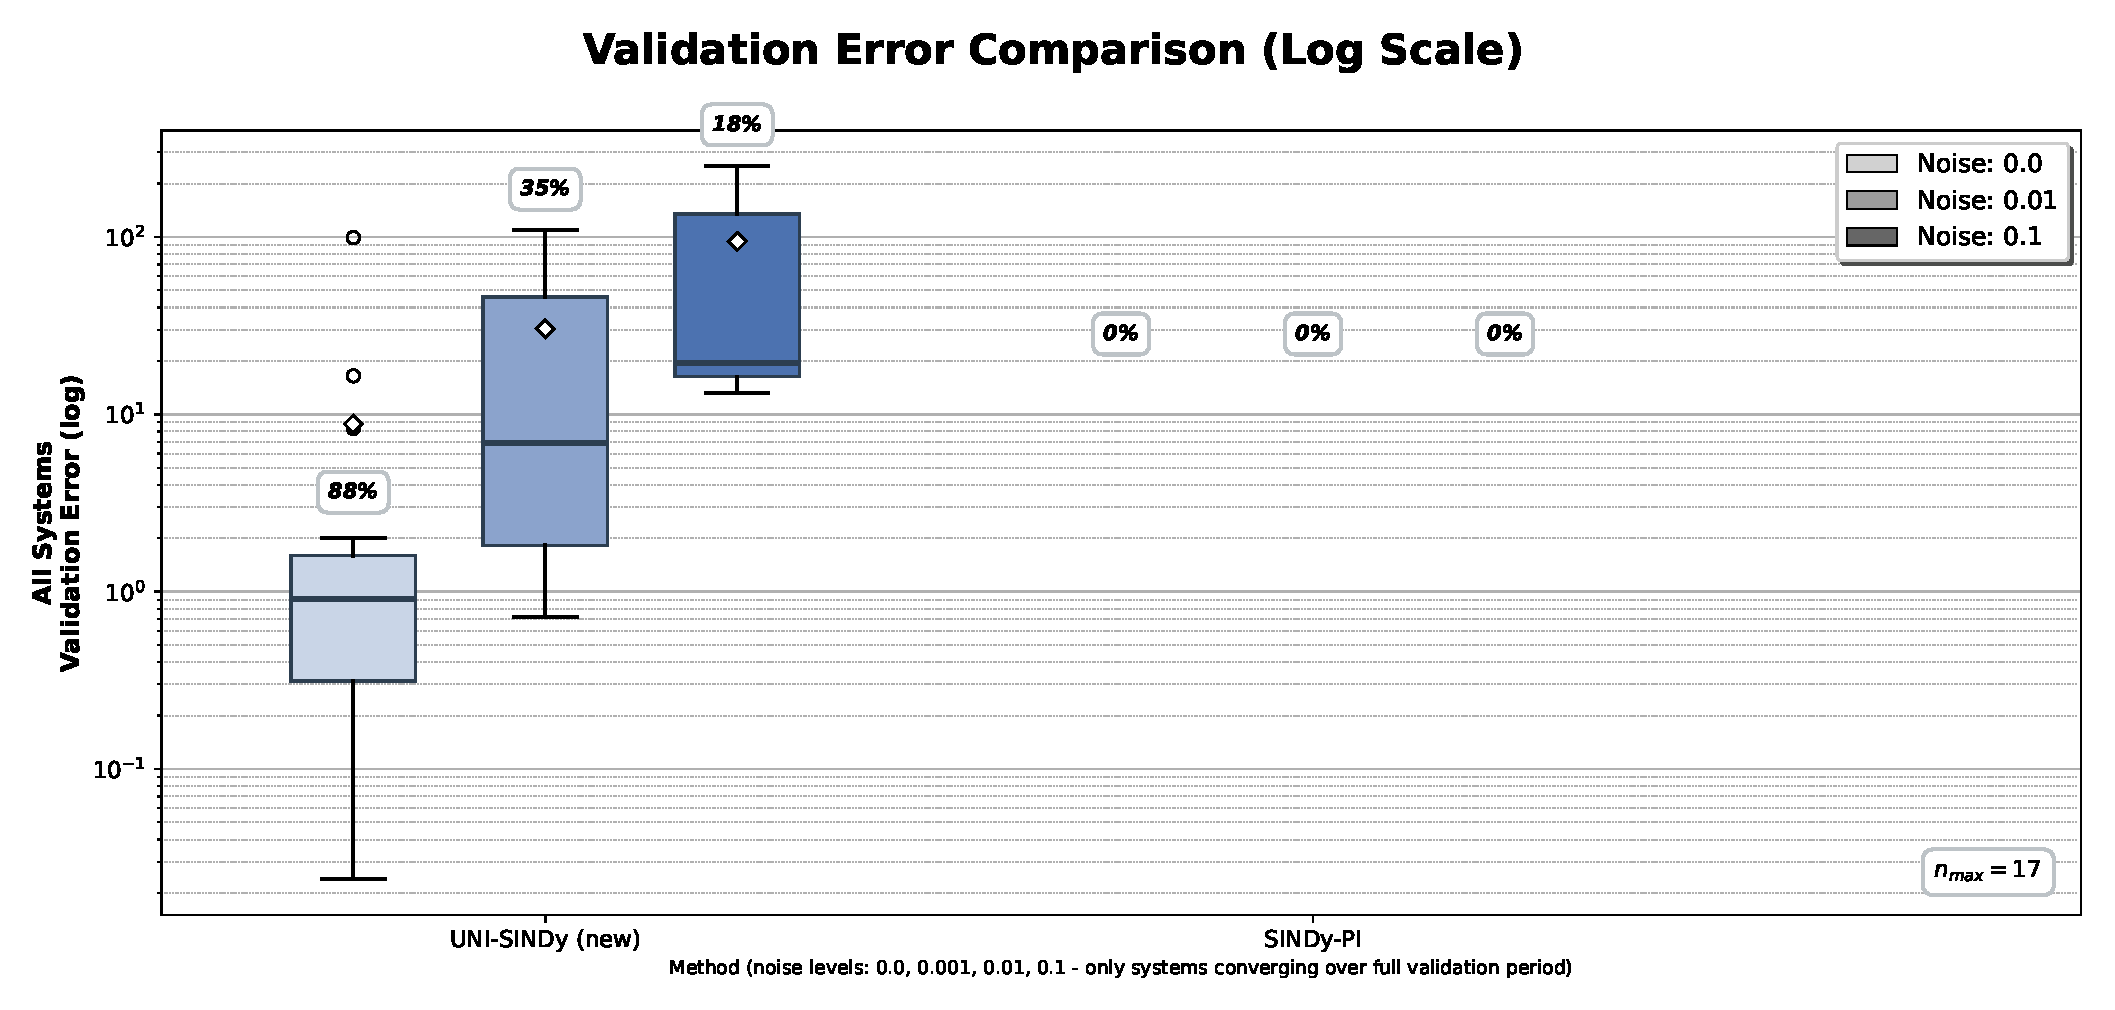
\includegraphics[width=0.95\textwidth]{result/plots_damping_implicit/noise_comparison_combined_white_background.eps}
    
    \vspace{0.5cm}
    
    \includegraphics[width=0.95\textwidth]{result/plots_damping_implicit/success_rate_combined_white_background.eps}
    
    \caption{\textbf{Any damping implicit results:} validation error comparison (top) and success rate comparison (bottom) across all systems}
    \label{fig:damping-implicit}
\end{figure}

\subsection{Any Damping Mixed Experiment}

This final experimental subset represents the most comprehensive aggregation of our testing protocols. It encompasses the entirety of the previously discussed scenarios—including fully explicit, fully implicit, damped, and undamped systems—while incorporating the novel "mixed" category. This specific class involves systems subjected to heterogeneous actuation topologies, where external forces are applied to only a subset of the generalized coordinates.

This category yields arguably the most significant results of our study, as it most accurately reflects the complex realities of physical robotic systems. Real-world platforms, ranging from walking humanoids to soft robots, frequently exhibit hybrid dynamics characterized by a combination of active joints (motors) and passive degrees of freedom (elasticity, unactuated linkages). As illustrated in Fig.~\ref{fig:damping-mixed}, Uni-SINDy demonstrates superior performance in this challenging domain, emerging as the most robust architecture in terms of identification success rate.

Regarding parameter accuracy, it is important to note that when the algorithms successfully converge, they perform on par with one another. This suggests that the limitation of standard methods is not the precision of the fit, but the ability to locate the correct sparse minimum within a vast search space. Uni-SINDy distinguishes itself not by fitting better, but by finding solutions in regimes where standard SINDy and SINDy-PI fail to converge entirely. Notably, Uni-SINDy was the \textit{only} algorithm capable of consistently discovering the governing dynamics for the highly complex, 3-DOF double-pendulum-on-cart system. This success validates the core hypothesis of this thesis: that the "Unified" approach, by leveraging a parsimonious Lagrangian library for internal dynamics and a targeted Newtonian library for inputs, effectively mitigates the combinatorial complexity that paralyzes traditional methods.

The overall complexity of this category is reflected in the statistics. Aggregating all 192 experiments resulted in a global "discarded experiment" rate of $61\%$—the highest among all test categories. This metric is heavily skewed by the inherent difficulty of the 3-DOF system. The combinatorial expansion of possible "active/passive" input configurations leads to many scenarios where the random forcing functions fail to sufficiently excite the unactuated coordinates, rendering the data uninformative. A breakdown of the discard rates by system topology illustrates this scaling of difficulty:

\begin{itemize}
    \item \textbf{Cartpole (2-DOF):} $35\%$ discarded experiments (17/48). Even with partial actuation, the system remains relatively easy to excite.
    \item \textbf{Double Pendulum (2-DOF):} $50\%$ discarded experiments (24/48). The chaotic nature of the system introduces stability challenges during data generation.
    \item \textbf{Cartpole Double (3-DOF):} $79\%$ discarded experiments (76/96). This significantly higher failure rate underscores the extreme challenge of identifying high-dimensional, under-actuated systems solely from random exploration, confirming that this system represents the current frontier for data-driven identification methods.
\end{itemize}

\begin{figure}[h]
    \centering
    \includegraphics[width=0.95\textwidth]{result/plots_damping_mixed/noise_comparison_combined_white_background.eps}
    
    \vspace{0.5cm}
    
    \includegraphics[width=0.95\textwidth]{result/plots_damping_mixed/success_rate_combined_white_background.eps}
    
    \caption{\textbf{Any damping implicit results:} validation error comparison (top) and success rate comparison (bottom) across all systems}
    \label{fig:damping-mixed}
\end{figure}

\section{Results on Real System}

To empirically validate the robustness of the proposed Uni-SINDy algorithm beyond the simulation environment, we constructed a physical experimental platform: a passive double pendulum, as illustrated in Fig.~\ref{fig:real-double-prendulum}. This system was fabricated using additive manufacturing (3D printing) to ensure rapid prototyping and reproducibility.

The dataset was constructed by aggregating approximately 100 seconds of experimental data derived from unforced, free-response trajectories. These experiments involved releasing the pendulum from a diverse set of initial angular configurations to ensure adequate phase-space coverage. To digitize the motion, we employed a custom computer-vision tracking algorithm. This pipeline extracted the raw Cartesian coordinates of the joint centers, from which the generalized coordinates (angles), velocities, and accelerations were derived. Special care was taken to apply smoothing filters during differentiation to mitigate the quantization noise inherent in visual tracking.

Utilizing this noisy real-world dataset, we applied the Uni-SINDy regression framework. The specific candidate library constructed for this analysis is detailed in Table~\ref{table:catalog-real-pendulum}.

\begin{table}
    \caption{Candidate function library utilized for the identification of the real double pendulum system.}
    \label{table:catalog-real-pendulum}
    \centering
    {
    \small
    \begin{tabular}{cl}
        \hline
        \textbf{Term \#} & \textbf{Expression} \\
        \hline
        \textbf{1}$^\dagger$ & $\dot{\theta}_1^2$ \\
        \textbf{2}$^\dagger$ & $\dot{\theta}_2^2$ \\
        3 & $\dot{\theta}_1 \dot{\theta}_2 \cos(\theta_1)$ \\
        4 & $\dot{\theta}_1 \dot{\theta}_2 \sin(\theta_1)$ \\
        5 & $\dot{\theta}_1 \dot{\theta}_2 \cos(\theta_2)$ \\
        6 & $\dot{\theta}_1 \dot{\theta}_2 \sin(\theta_2)$ \\
        7 & $\dot{\theta}_1 \dot{\theta}_2 \cos(\theta_1) \sin(\theta_2)$ \\
        8 & $\dot{\theta}_1 \dot{\theta}_2 \sin(\theta_1) \cos(\theta_2)$ \\
        9 & $\dot{\theta}_1 \dot{\theta}_2 \cos(\theta_1) \cos(\theta_2)$ \\
        10 & $\dot{\theta}_1 \dot{\theta}_2 \sin(\theta_1) \sin(\theta_2)$ \\
        11 & $\cos(\theta_1)$ \\
        12 & $\cos(\theta_2)$ \\
        13 & $\sin(\theta_1)$ \\
        \hline
    \end{tabular}
    \hspace{1ex}
    \begin{tabular}{cl}
        \hline
        \textbf{Term \#} & \textbf{Expression} \\
        \hline
        14 & $\sin(\theta_2)$ \\
        15 & $\cos(\theta_1) \sin(\theta_2)$ \\
        16 & $\sin(\theta_1) \cos(\theta_2)$ \\
        17 & $\cos(\theta_1) \cos(\theta_2)$ \\
        18 & $\sin(\theta_1) \sin(\theta_2)$ \\
        19 & $\dot{\theta}_1 \cos(\theta_1)$ \\
        20 & $\dot{\theta}_1 \cos(\theta_1)$ \\
        21 & $\dot{\theta}_1 \cos(\theta_1)$ \\
        22 & $\dot{\theta}_1 \cos(\theta_1)$ \\
        23 & $\dot{\theta}_2 \cos(\theta_1)$ \\
        24 & $\dot{\theta}_2 \cos(\theta_1)$ \\
        25 & $\dot{\theta}_2 \cos(\theta_1)$ \\
        26 & $\dot{\theta}_2 \cos(\theta_1)$ \\
        \hline
    \end{tabular}
    }

    \raggedright
    \vspace{0.5ex}
    $\dagger$ : Pre-knowledge term designated for the regression.

\end{table}

It is important to highlight a specific methodological deviation employed here: although the system is physically passive (no motor inputs), we did not enforce a strictly implicit regression for all terms. Instead, we designated the kinetic energy scaling terms ($\dot{\theta}_1^2, \dot{\theta}_2^2$) as "pre-knowledge" or fixed regressors. This decision was necessitated by the extreme scaling disparity present in the physical system. Due to the mass distribution and arm lengths, the gravitational torque terms exhibited amplitudes approximately 300 times larger than the inertial and Coriolis terms. Without anchoring the regression with pre-knowledge, the optimization landscape becomes ill-conditioned, leading the algorithm to neglect the subtle inertial dynamics in favor of fitting the dominant gravity vector.

\begin{figure}
    \centering
    \includegraphics[width=0.8\textwidth]{figures/real_double_pendulum.png}
    \caption{\textbf{Experimental Double Pendulum Setup:} The system is constructed from PLA 3D-printed components. To minimize unmodeled non-linearities, the joints are outfitted with precision bearings from which the factory high-viscosity grease was chemically removed to guarantee the lowest possible friction coefficient.}
    \label{fig:real-double-prendulum}
\end{figure}

To rigorously mitigate the risk of overfitting—a pervasive issue when identifying models from noisy sensor data—we enforced a strict data aspect ratio of $1.5$. Practically, this implies that the optimization was constrained to use only $39$ discrete time samples extracted from the $100$ seconds of available training data. Despite this extreme subsampling, the algorithm converged to a sparse model comprising $13$ active terms. 

The predictive fidelity of this model is visualized in Fig.~\ref{fig:result-real-pendulum}, which depicts a 1-second forecast horizon. It must be noted that for a double pendulum, which is an inherently chaotic system sensitive to initial conditions (positive Lyapunov exponent), a one-second horizon represents a significant duration. The ability to track the real system over this interval indicates that the model has successfully captured the complex inertial coupling, rather than just the first-order gravity terms.

\begin{figure}
    \centering
    \includegraphics[width=0.8\textwidth]{figures/result_real_pendulum.png}
    \caption{\textbf{Validation of Real System Identification:} A comparison between the ground truth trajectory of the physical system and a 1-second open-loop forecast generated by the identified model, initialized from a random state.}
    \label{fig:result-real-pendulum}
\end{figure}

To further validate the generalization capability of the model, we recorded a separate validation video sequence. We extracted multiple distinct initial conditions along this trajectory, generated forecasts, and compared them against the observed physical motion (as shown in Fig.~\ref{fig:result-real-pendulum}). Across multiple trials, the retrieved equations consistently captured the true dynamics. A secondary structural analysis of the identified coefficients confirmed the presence of the expected macro-terms governing rigid body mechanics, specifically the trigonometric cross-coupling terms and the gravitational potential components.

Current ongoing research focuses on the integration of the Uni-SINDy estimator into a closed-loop control framework. A final experiment is currently under development to demonstrate real-time model predictive control of a mixed passive-active system (specifically, the cartpole and double pendulum on a cart). These results, which aim to definitively demonstrate the superiority of Uni-SINDy for under-actuated robotics, will be detailed in a forthcoming manuscript currently in preparation.


% -------------------------------------------------------------------------
%   CHAPTER: DISCUSSION
% -------------------------------------------------------------------------

\cleardoublepage
\chapter{Discussion}
\label{ch:discussion}

The central hypothesis of this thesis posited that the effective identification of modern robotic systems requires a hybrid modeling approach—one that bridges the divide between the structural parsimony of Lagrangian mechanics and the modular flexibility of Newtonian formulations. The development and validation of the UNI-SINDy framework have provided substantial empirical evidence supporting this view.

In this chapter, we interpret the results presented in Chapter \ref{ch:results}, analyzing the mechanisms that allowed UNI-SINDy to succeed in regimes where established methods faltered. We further discuss the implications of the "Mixed" identification strategy for the broader field of robotics, while candidly addressing the limitations and boundaries of the current framework.

\section{Overcoming the Curse of Dimensionality through Structural Priors}

The most significant finding of this study is the scalability of the Unified Catalog compared to standard Newtonian approaches. As demonstrated in the \textit{Any Damping Implicit} experiments, the standard SINDy-PI algorithm failed to identify the dynamics for the Cartpole and Double Pendulum systems, yielding a 0\% success rate. This failure was not due to a lack of theoretical capability, but rather a "curse of dimensionality" inherent to the unbiased Newtonian formulation.

By adhering to the "equivalent input knowledge" protocol, the Newtonian library was forced to span the full polynomial space required to cover the dynamics. For a multi-degree-of-freedom system, this results in a combinatorial explosion of candidate terms. The regression algorithm is essentially tasked with finding a needle in a haystack of thousands of correlated functions.

In contrast, the UNI-SINDy framework leverages the strong inductive bias of the Lagrangian formulation. By solving for a scalar energy function ($L$) rather than a vector field of accelerations, we reduced the search space by an order of magnitude (as detailed in Table \ref{table:catalog-size}). Effectively, the Euler-Lagrange operator acts as a "physics-informed filter," automatically enforcing the coupling between inertial terms that standard SINDy must "learn" from scratch. This result suggests that in high-dimensional mechanical systems, the injection of structural physical priors is not merely an optimization trick, but a prerequisite for tractability.

\section{The Efficacy of the Mixed Implicit-Explicit Algorithm}

The "Mixed" experiments highlighted the limitations of treating system identification as a binary choice between Explicit ($\dot{x} = f(x,u)$) and Implicit ($F(\dot{x}, x) = 0$) regression. Real robotic systems, particularly those with under-actuation or flexible joints, exist on a spectrum between these two poles.

The superior performance of UNI-SINDy in the \textit{Cartpole Double} experiment (the most complex 3-DOF case) validates the recursive logic of our proposed Mixed Algorithm. By first identifying the "Actuated Subspace" (Explicit step), the algorithm effectively "cleans" the residual signal before attempting to solve the harder Implicit problem. This divide-and-conquer strategy serves two purposes:
\begin{enumerate}
    \item \textbf{Numerical Stability:} It prevents the strong signals from actuated joints (e.g., motor torques) from overshadowing the subtle passive dynamics in the regression.
    \item \textbf{Search Space Reduction:} By removing identified terms from the active library, the subsequent implicit step operates on a significantly smaller matrix, reducing the risk of convergence to trivial null-space solutions.
\end{enumerate}

This finding is particularly relevant for the control of soft robots or floating-base humanoids, where the boundary between active actuation and passive environmental interaction is often blurred.

\section{Real-World Robustness and the "Dominant Dynamics" Problem}

The experimental validation on the physical passive double pendulum exposed a critical challenge often masked by simulation: the issue of scale disparity. In our physical setup, the gravitational torques were approximately 300 times larger than the inertial and Coriolis terms.

In a standard "blind" regression, optimization algorithms (like LASSO) tend to latch onto these dominant features (gravity) while zeroing out the smaller coefficients (inertia) to minimize the sparsity penalty. This results in a model that is statistically accurate but physically broken—capable of predicting static equilibrium but failing to capture motion.

The success of the real-world identification relied on the strategic use of "Pre-knowledge" within the Unified Catalog. By forcing the inclusion of specific kinetic energy terms ($\dot{\theta}^2$), we effectively anchored the regression, compelling the optimizer to fit the residual dynamics around the known inertial structure. This highlights a key advantage of the "White Box" approach: unlike Neural Networks, where internal weights are opaque, UNI-SINDy allows the engineer to manually inject domain expertise to stabilize the solution against signal-to-noise imbalances.

\section{Limitations}

Despite the promising results, the current iteration of UNI-SINDy is subject to several limitations that must be acknowledged.

\subsection{Dependency on Derivative Quality}
Like all SINDy-based approaches, our framework is strictly dependent on the availability of high-quality state derivatives ($\dot{q}, \ddot{q}$). In our physical experiments, we relied on smoothed differentiation of computer vision data. However, in systems with high-frequency noise or quantization errors (e.g., low-resolution encoders), the numerical calculation of acceleration can amplify noise to unusable levels. While integral-form SINDy formulations exist in the literature, they have not yet been adapted to the Lagrangian formalism used here.

\subsection{Catalog Completeness and Friction Models}
The "Unified" nature of our catalog assumes that the true dynamics can be represented as a linear combination of the provided basis functions. While the Lagrangian sub-catalog handles rigid body dynamics robustly, the Newtonian sub-catalog relies on the user to populate it with appropriate friction models (Coulomb, Viscous, Stribeck). If the physical system exhibits complex hysteretic friction or non-polynomial aerodynamic drag that is not present in the library, the algorithm will fail to capture these effects, potentially compensating by overfitting other terms.

\subsection{Computational Cost of the Symbolic Engine}
While the regression step is efficient, the symbolic construction of the Lagrangian library involves applying the Euler-Lagrange operator to a symbolic expression. As the number of degrees of freedom increases, the symbolic length of the equations of motion grows exponentially. For systems with $N > 10$ DOF, the time required to generate the library matrix $\boldsymbol{\Theta}$ may become a bottleneck, necessitating more efficient symbolic engines or automatic differentiation techniques.

\section{Implications for Robotics and Future Work}

The ability to extract interpretable, physics-based models from data opens significant avenues for future research.

The most immediate application is in Model Predictive Control (MPC). The equations discovered by UNI-SINDy are sparse and explicit, making them ideal candidates for real-time optimization solvers that require rapid gradient computation. Future work will focus on closing the loop: running UNI-SINDy online to adaptively update the model of a robot as it interacts with unknown environments (e.g., picking up a heavy object).

Furthermore, the framework could be extended to the domain of Soft Robotics. By incorporating basis functions derived from continuum mechanics or finite element approximations into the Unified Catalog, it may be possible to discover reduced-order models for soft actuators that are currently treated as black boxes.

In conclusion, this thesis demonstrates that by respecting the distinct physical nature of conservative and dissipative forces, and by unifying them into a coherent mathematical framework, we can achieve data-driven identification that is both robust and interpretable.


% -------------------------------------------------------------------------
% CHAPTER: CONCLUSION
% -------------------------------------------------------------------------

\cleardoublepage
\chapter{Conclusion}
\label{ch:conclusion}

The precise modeling of dynamical systems is the bedrock upon which the safety, efficiency, and autonomy of robotic agents are built. As we move towards increasingly complex architectures—from under-actuated manipulators to compliant soft robots—the limitations of classical analytical derivation and the opacity of modern "black-box" machine learning become increasingly apparent. This thesis set out to navigate the space between these two extremes, aiming to develop a data-driven identification framework that is as flexible as a neural network yet as interpretable as a textbook derivation.

The primary contribution of this work is the realization of \textbf{UNI-SINDy} (Unified Simultaneous Lagrangian and Newtonian Identification). This framework was born from the observation that robotic systems are rarely monolithic; they are "mixed" entities governed simultaneously by conservative energy exchanges and non-conservative dissipative forces, and characterized by topologies that blend active control with passive dynamics. Existing methods in the literature, while powerful in isolation, often forced a binary choice: the structural rigidity of Lagrangian identification or the dimensional explosion of Newtonian regression.

\section*{Summary of Contributions}

To bridge this gap, we introduced three fundamental innovations. First, the \textbf{Unified Catalog} fundamentally restructures the regression problem. By allowing the coexistence of Lagrangian energy candidates (processed via the Euler-Lagrange operator) and Newtonian force terms within a single experiment matrix, we enabled the simultaneous identification of inertial parameters and friction models. This approach leverages the extreme compactness of the Lagrangian scalar formulation—effectively injecting physical prior knowledge to combat the curse of dimensionality—while retaining the freedom to describe arbitrary non-conservative phenomena.

Second, we developed the \textbf{Mixed Implicit-Explicit Algorithm}. This recursive algorithm provides a structured pathway to disentangle active dynamics from passive constraints. By systematically resolving the "known" explicit subspace before tackling the "hidden" implicit dynamics, the algorithm drastically reduces the computational burden and numerical instability associated with null-space regression.

Third, we enhanced the robustness of the solution selection process through \textbf{Information-Theoretic Clustering}. By moving beyond simple sparsity metrics and analyzing the geometric clustering of candidate vectors, we addressed the issue of disjoint subspaces, ensuring that the identified equations represent physically consistent global dynamics rather than local numerical artifacts.

\section*{Synthesis of Findings}

The validity of these contributions was confirmed through a rigorous comparative analysis against established baselines (Standard SINDy, SINDy-PI, and XL-SINDy). In simulation, UNI-SINDy demonstrated a distinct superiority in handling high-dimensional, under-actuated systems. Notably, in the challenging case of the triple-link "Cartpole Double" system, our framework successfully identified the governing equations where standard Implicit SINDy (SINDy-PI) failed completely. This failure of the baseline was traced to the combinatorial explosion of the unbiased Newtonian library, highlighting the necessity of the structural priors inherent in our Unified approach.

Furthermore, the transition from simulation to reality provided the ultimate validation. The successful identification of a physical, 3D-printed passive double pendulum from noisy video data demonstrated the practical utility of the framework. This experiment specifically highlighted the importance of allowing "pre-knowledge" injection within the regression to handle the scale disparity between dominant gravitational forces and subtle inertial couplings—a nuance that purely automated black-box methods often miss.

\section*{Final Outlook}

In conclusion, this thesis presents a compelling argument for the adoption of "White Box" physics-informed machine learning in robotics. We have demonstrated that it is possible to discover complex, non-linear equations of motion directly from data without sacrificing interpretability. The UNI-SINDy framework provides engineers with a mathematical description of the system that can be directly analyzed for stability, utilized in optimal control solvers, and verified for safety compliance.

While challenges remain—specifically regarding the dependency on high-quality derivative data and the symbolic scalability for hyper-redundant systems—this work lays a solid foundation for future research. By providing a tool that "speaks the language" of physics, we take a significant step closer to robotic systems that not only learn how to move but understand the laws that govern their motion.


\chapter*{Acknowledgements}

While this thesis marks the conclusion of my Master's degree, it represents a journey that I could not have undertaken alone.

I would like to extend my sincere appreciation to my supervisor, Professor Hayashibe, for accepting me into his laboratory. Over the past two and a half years, his mentorship has been pivotal, allowing me to navigate life in Japan and dive deeply into the research world. The autonomy I was afforded during this time was invaluable, providing me the space to explore this field creatively and broaden my technical horizons.

I also owe a debt of gratitude to my partner, whom I was lucky to meet during this program. Thank you for the time we spent working side by side; your support provided the essential energy and drive required to reach this finish line.

To my family and friends, thank you for your unwavering support and for believing in my potential. You have kept me grounded and motivated throughout every step of this process.

Lastly, I wish to acknowledge the open-source community. As the saying goes, we stand on the shoulders of giants; without the collaborative spirit and the tools shared by previous researchers, this work would not have been possible.

% -------------------------------------------------------------------------
%   BACK MATTER
% -------------------------------------------------------------------------

\printbibliography

\appendix
\chapter{Python Implementation}

\begin{lstlisting}[language=Python, caption={\textbf{Weak sparsity function}}, label=lst:weak-sparsity]
def _weak_sparsity_rank_weighted(x):

    x = np.abs(x)
    s = np.sort(x)[::-1] # descending order
    ranks = np.arange(1, len(s) + 1)

    weights = 1.0 / ranks
    weighted_sum = np.sum(s * weights)
    weight_total = np.sum(s)

    if weight_total == 0:
        return 0
    else:
        return weighted_sum / weight_total

\end{lstlisting}

\chapter{All data figures}
\label{ch:all-result-figures}

\section{Damping Explicit Results}

\begin{figure}[H]
    \centering
    \begin{subfigure}[b]{0.95\textwidth}
        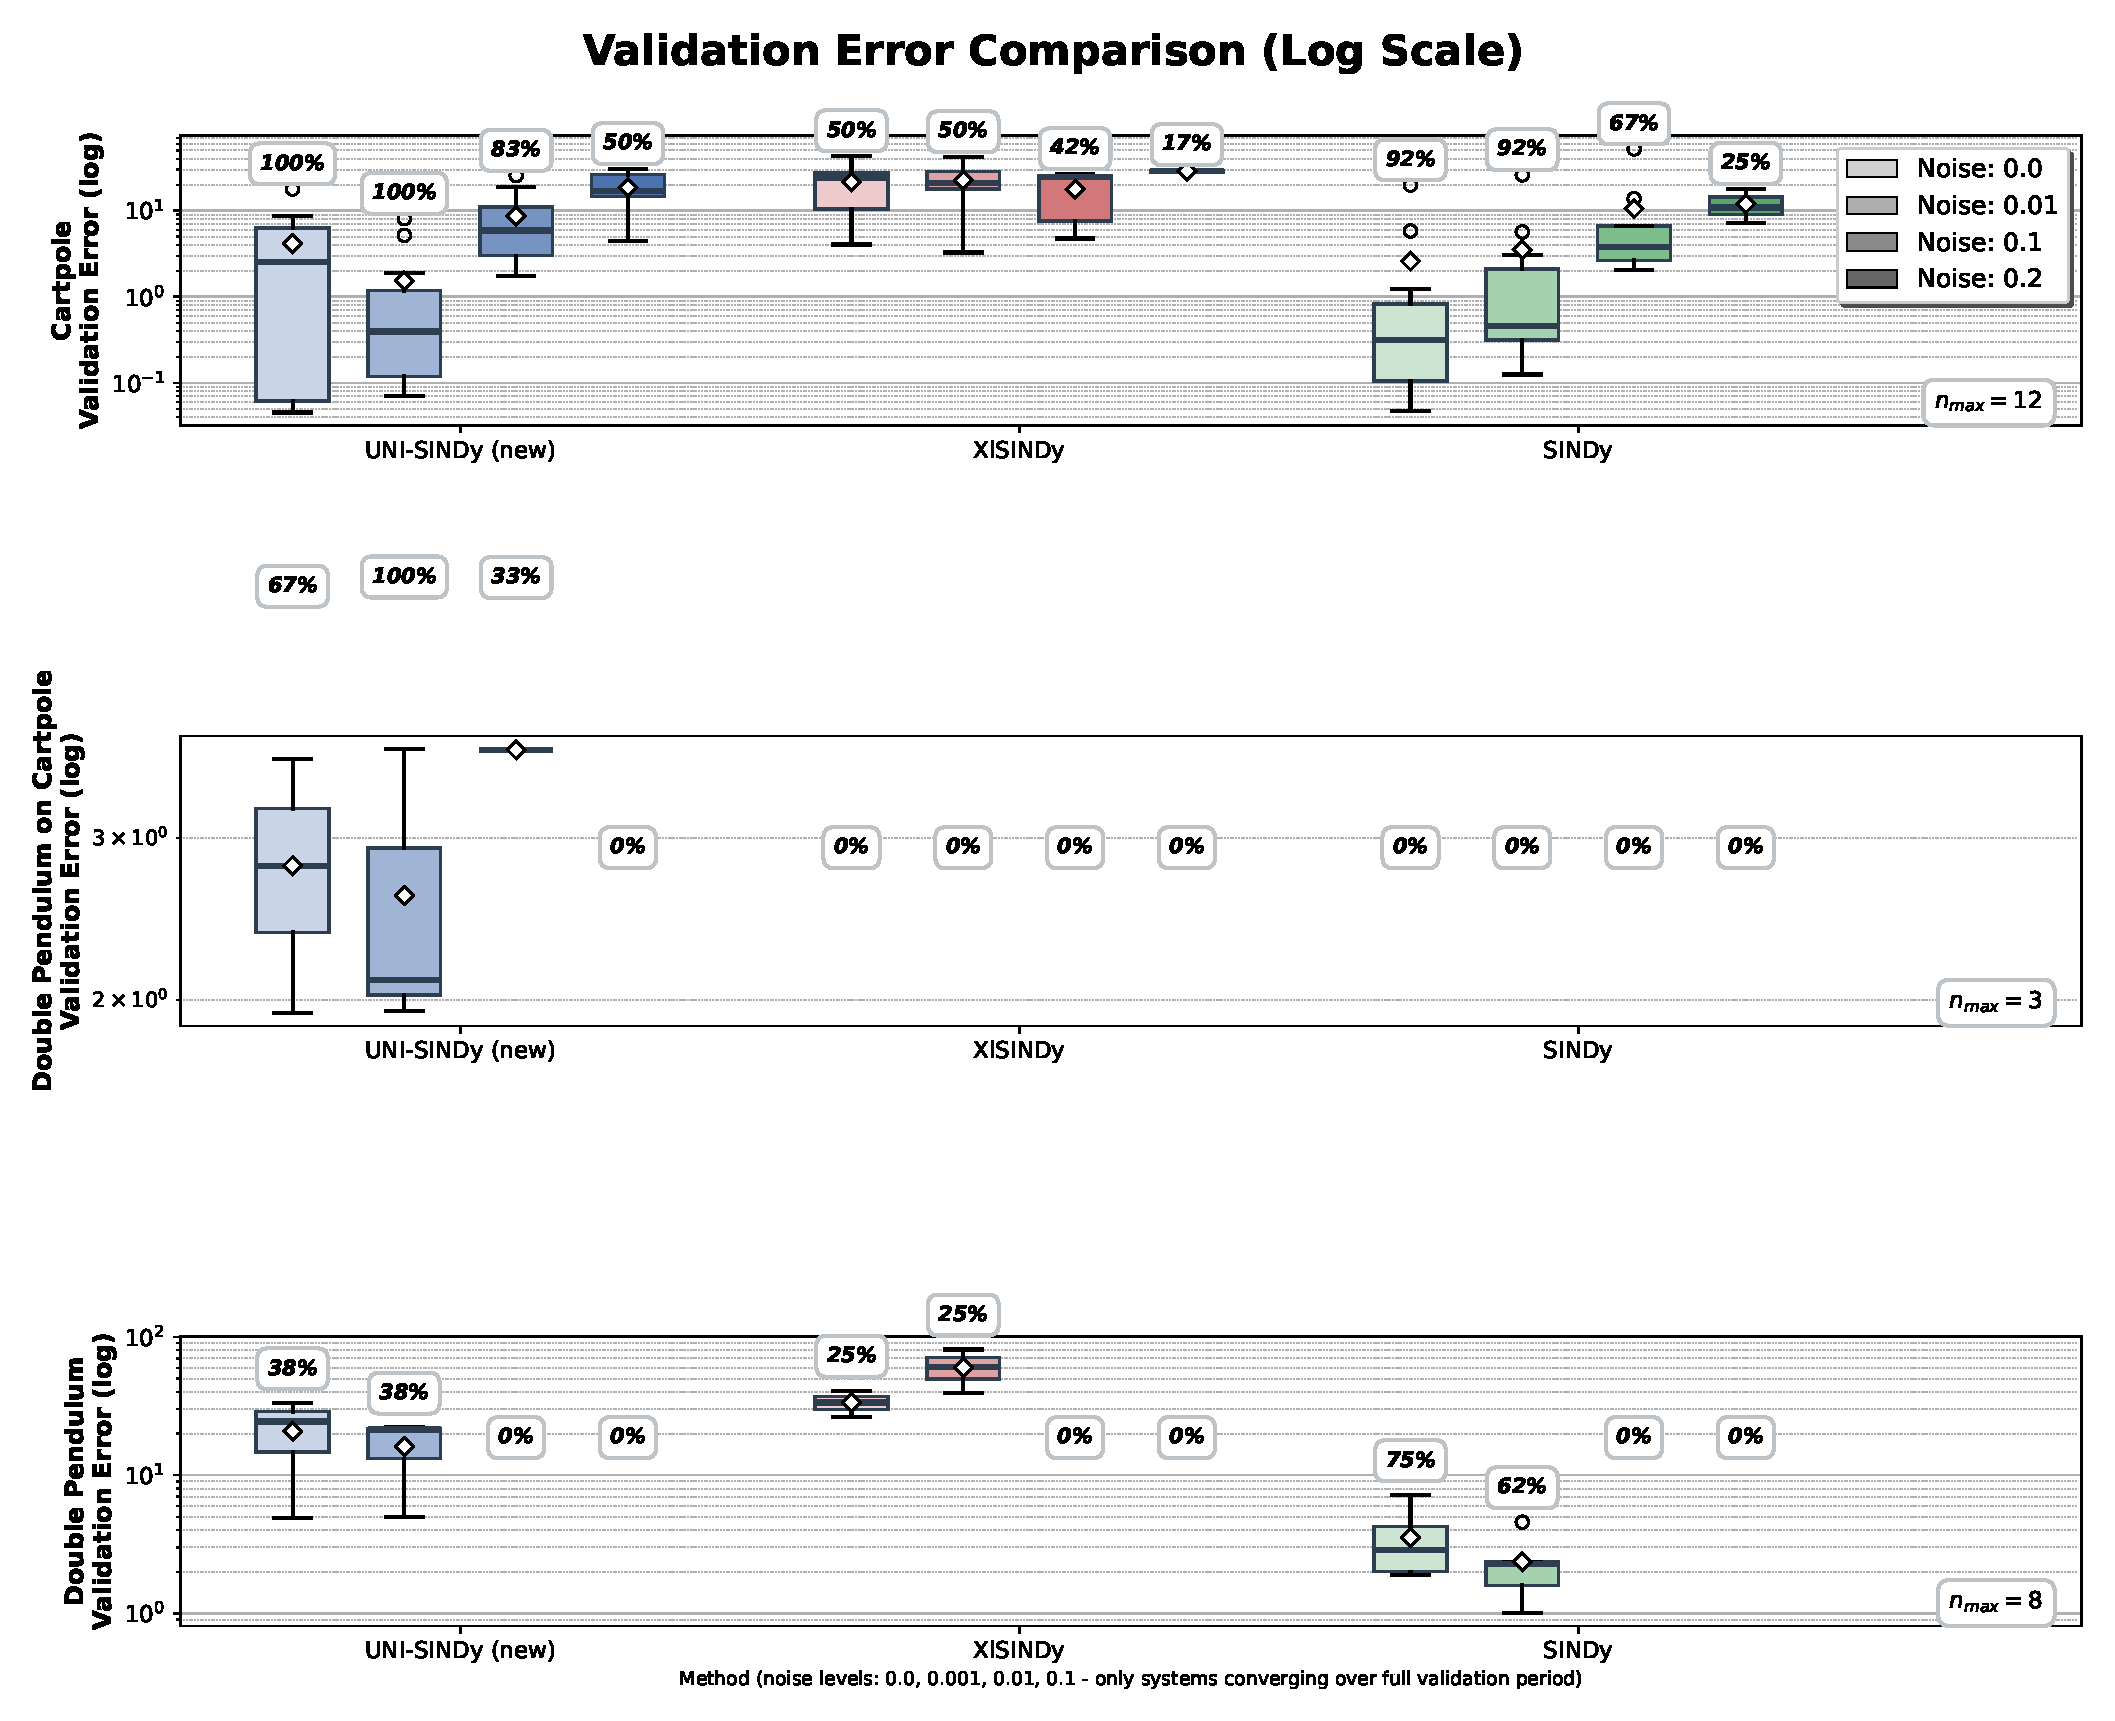
\includegraphics[width=\textwidth]{result/plots_damping_explicit/noise_comparison_white_background.eps}
        \caption{Noise comparison}
    \end{subfigure}
    
    \vspace{0.5cm}
    
    \begin{subfigure}[b]{0.95\textwidth}
        \includegraphics[width=\textwidth]{result/plots_damping_explicit/noise_comparison_combined_white_background.eps}
        \caption{Noise comparison combined}
    \end{subfigure}
    \caption{Damping explicit - Validation error comparison}
    \label{fig:damping_explicit_validation}
\end{figure}

\begin{figure}[H]
    \centering
    \begin{subfigure}[b]{0.95\textwidth}
        \includegraphics[width=\textwidth]{result/plots_damping_explicit/success_rate_white_background.eps}
        \caption{Success rate}
    \end{subfigure}
    
    \vspace{0.5cm}
    
    \begin{subfigure}[b]{0.95\textwidth}
        \includegraphics[width=\textwidth]{result/plots_damping_explicit/success_rate_combined_white_background.eps}
        \caption{Success rate combined}
    \end{subfigure}
    \caption{Damping explicit - Success rate comparison}
    \label{fig:damping_explicit_success}
\end{figure}

\section{Damping Implicit Results}

\begin{figure}[H]
    \centering
    \begin{subfigure}[b]{0.95\textwidth}
        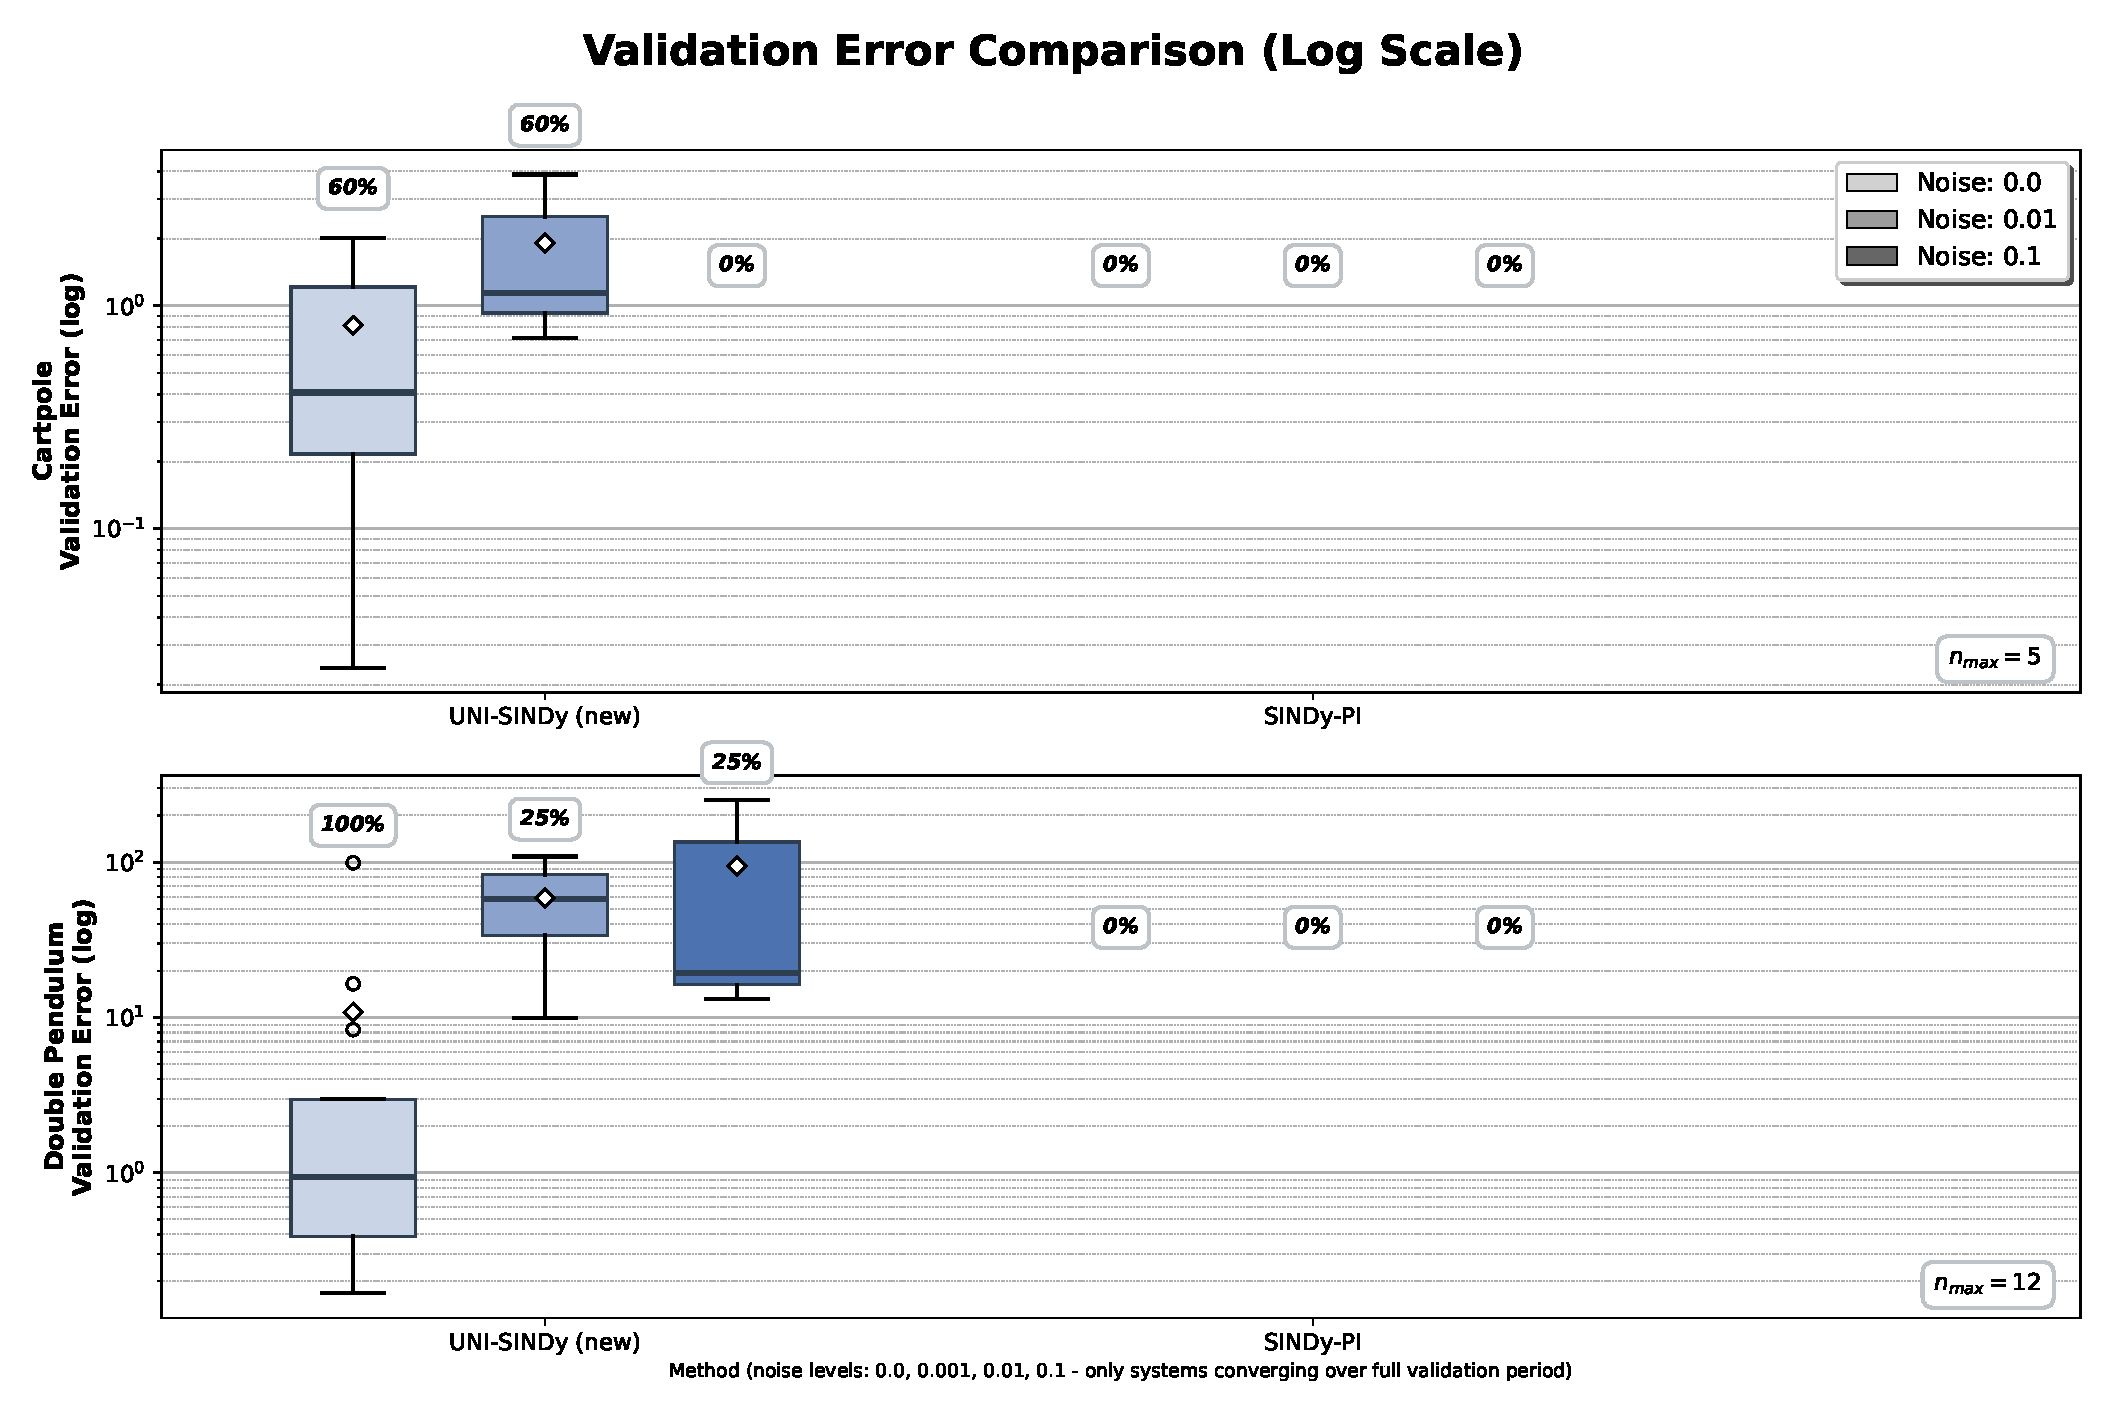
\includegraphics[width=\textwidth]{result/plots_damping_implicit/noise_comparison_white_background.eps}
        \caption{Noise comparison}
    \end{subfigure}
    
    \vspace{0.5cm}
    
    \begin{subfigure}[b]{0.95\textwidth}
        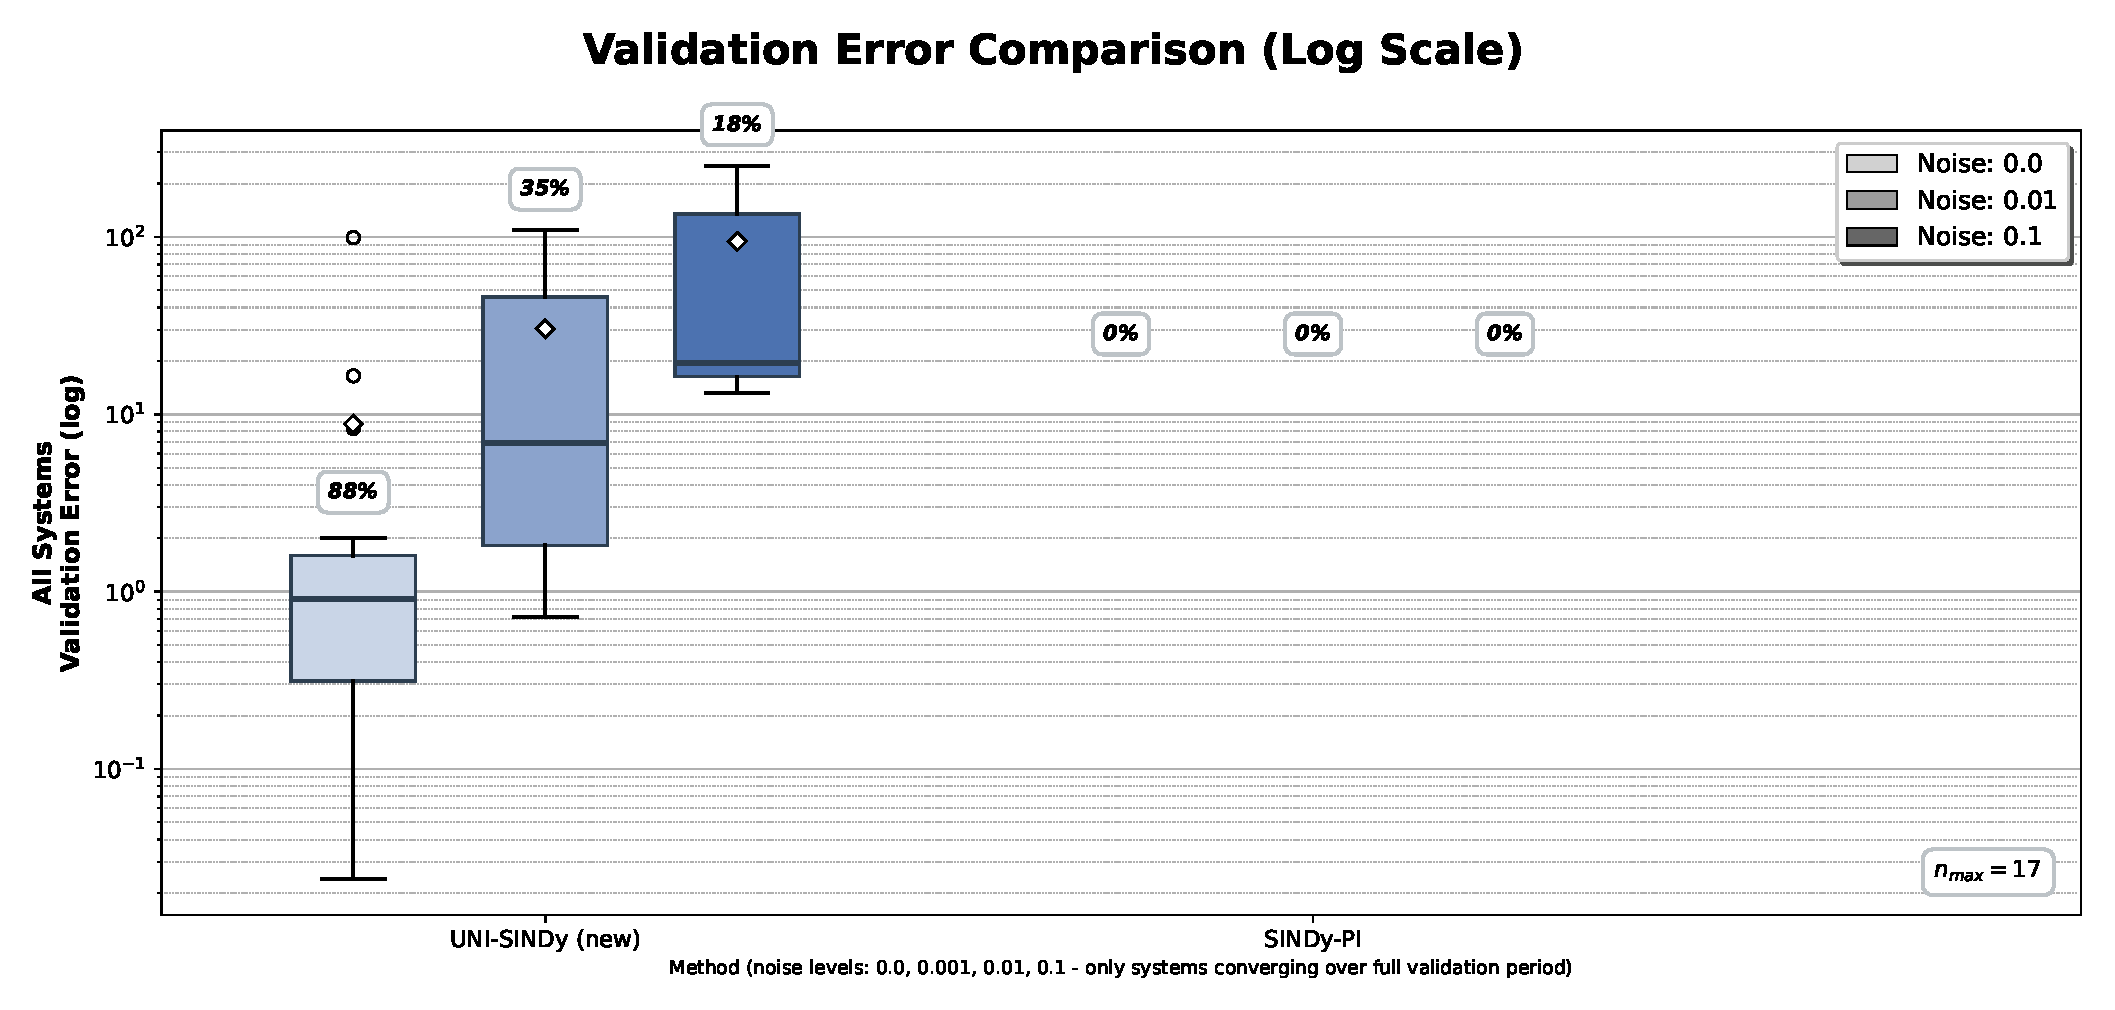
\includegraphics[width=\textwidth]{result/plots_damping_implicit/noise_comparison_combined_white_background.eps}
        \caption{Noise comparison combined}
    \end{subfigure}
    \caption{Damping implicit - Validation error comparison}
    \label{fig:damping_implicit_validation}
\end{figure}

\begin{figure}[H]
    \centering
    \begin{subfigure}[b]{0.95\textwidth}
        \includegraphics[width=\textwidth]{result/plots_damping_implicit/success_rate_white_background.eps}
        \caption{Success rate}
    \end{subfigure}
    
    \vspace{0.5cm}
    
    \begin{subfigure}[b]{0.95\textwidth}
        \includegraphics[width=\textwidth]{result/plots_damping_implicit/success_rate_combined_white_background.eps}
        \caption{Success rate combined}
    \end{subfigure}
    \caption{Damping implicit - Success rate comparison}
    \label{fig:damping_implicit_success}
\end{figure}

\section{Damping Mixed Results}

\begin{figure}[H]
    \centering
    \begin{subfigure}[b]{0.95\textwidth}
        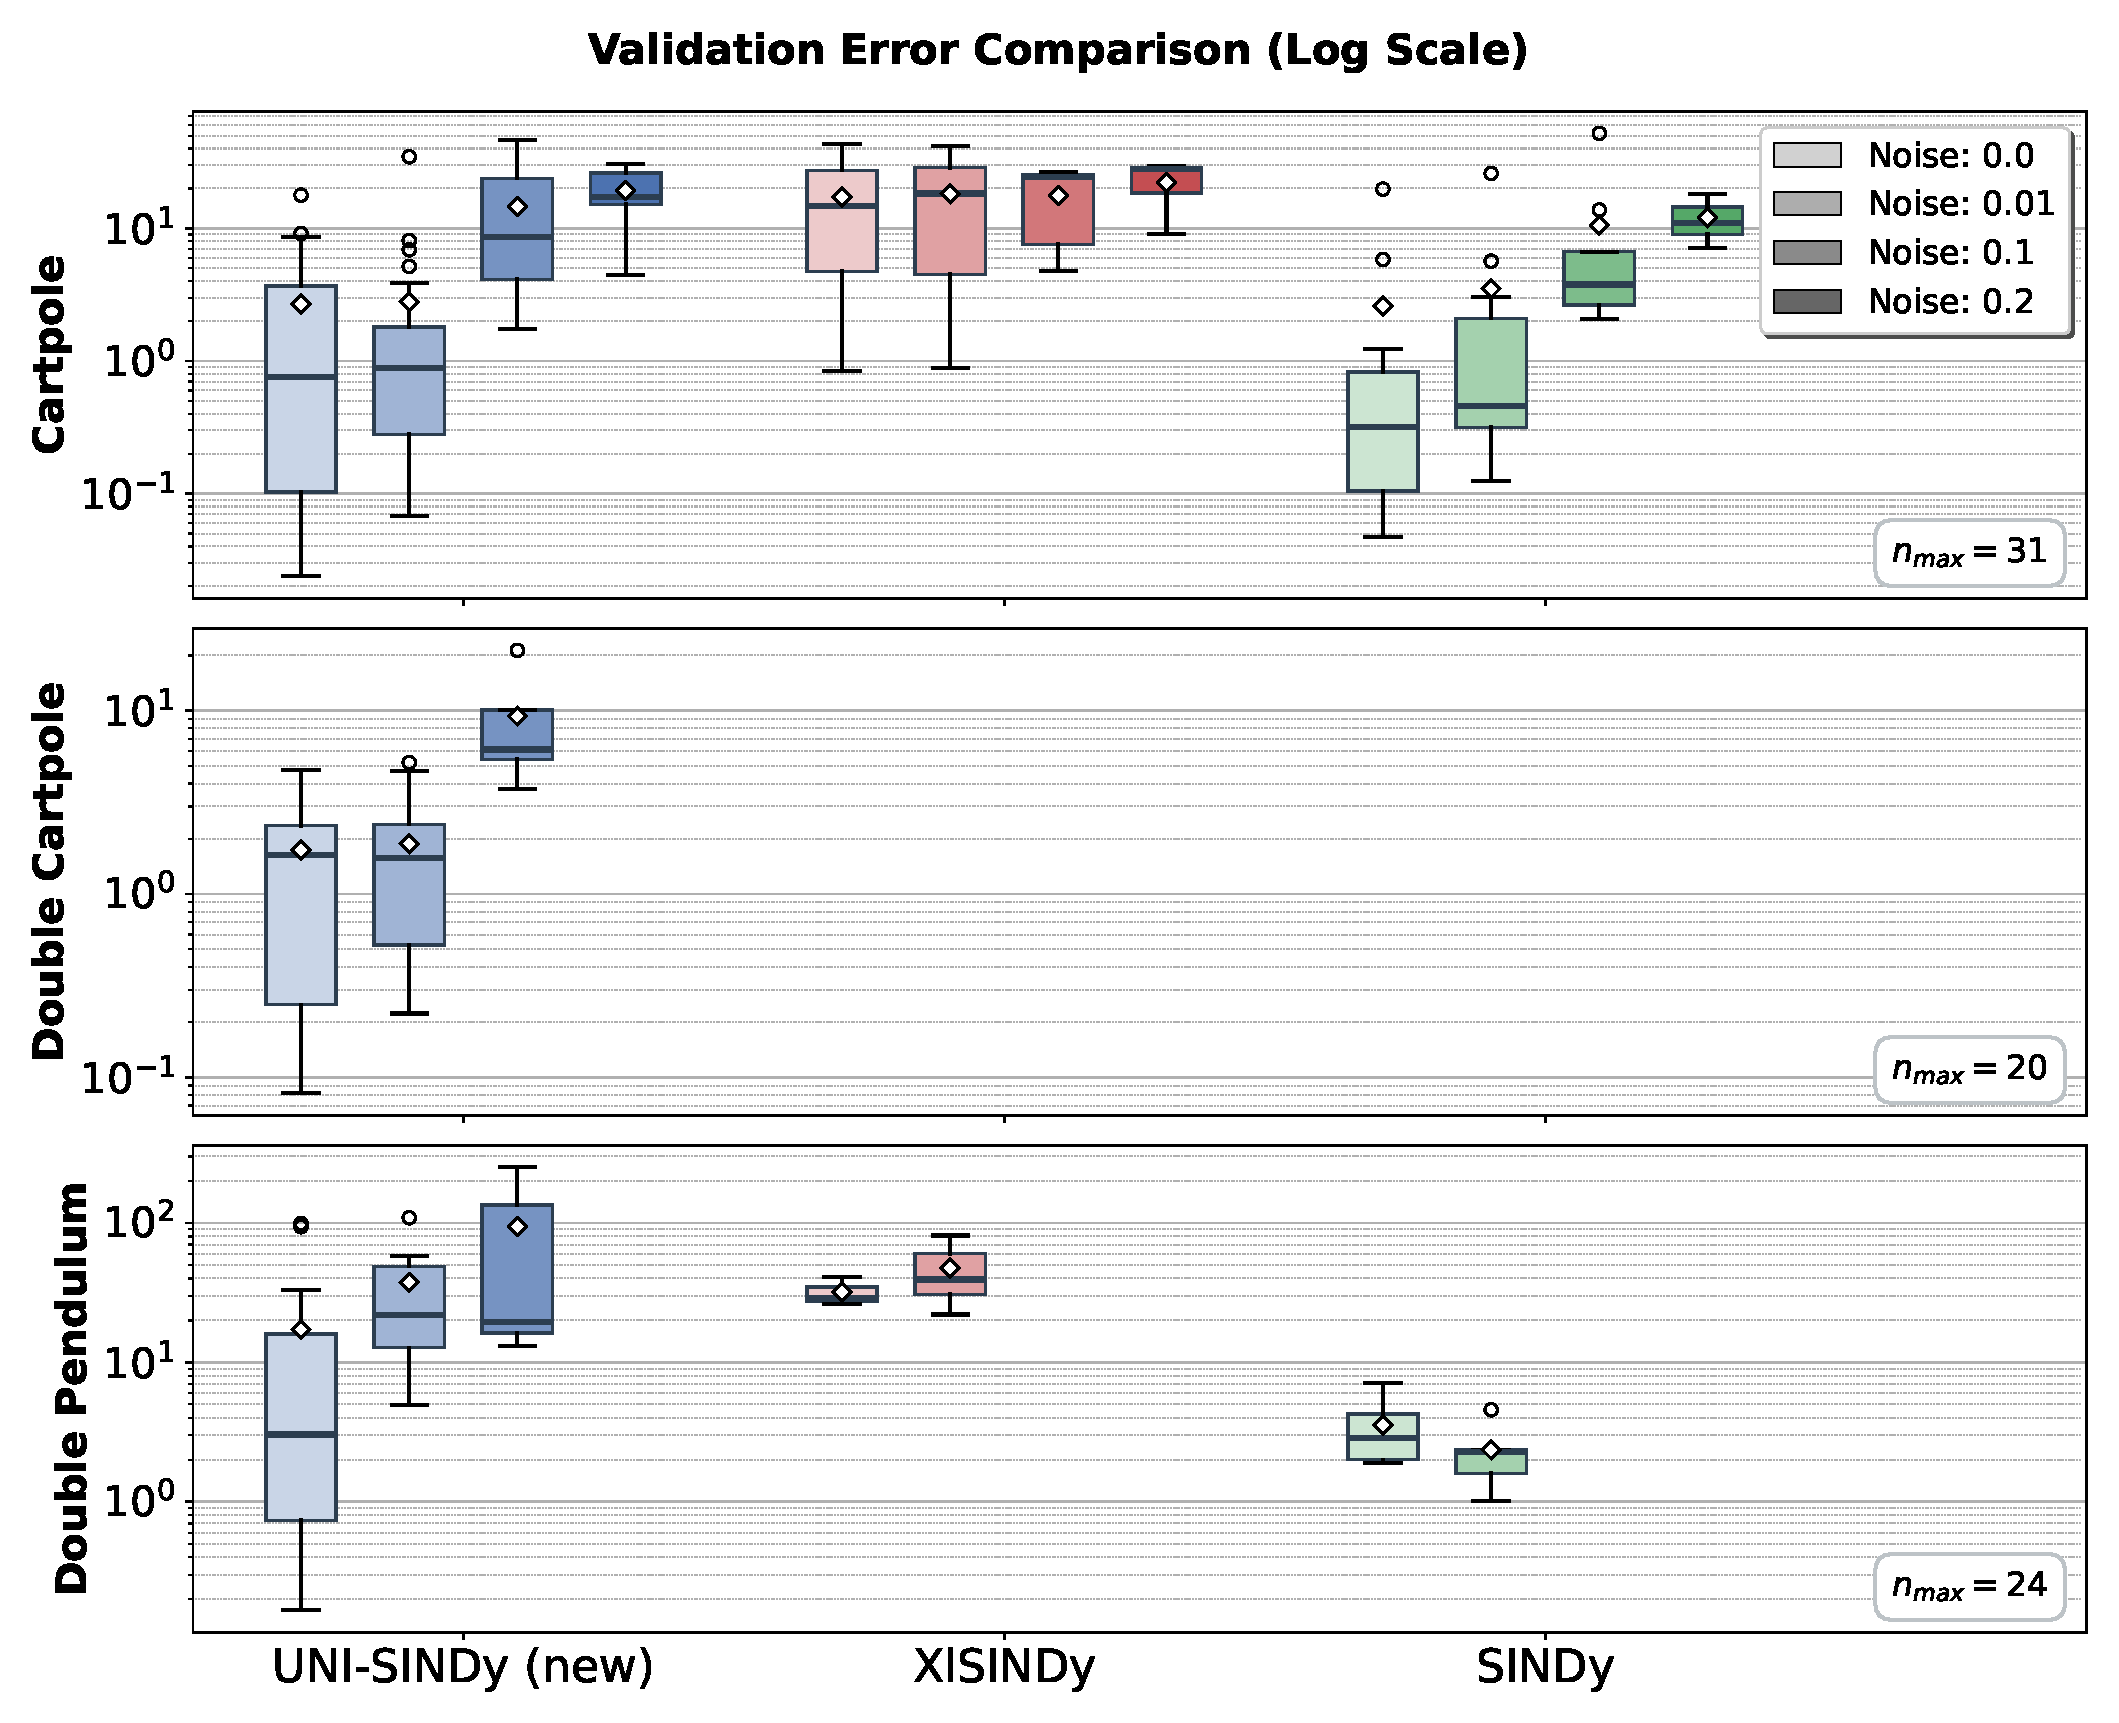
\includegraphics[width=\textwidth]{result/plots_damping_mixed/noise_comparison_white_background.eps}
        \caption{Noise comparison}
    \end{subfigure}
    
    \vspace{0.5cm}
    
    \begin{subfigure}[b]{0.95\textwidth}
        \includegraphics[width=\textwidth]{result/plots_damping_mixed/noise_comparison_combined_white_background.eps}
        \caption{Noise comparison combined}
    \end{subfigure}
    \caption{Damping mixed - Validation error comparison}
    \label{fig:damping_mixed_validation}
\end{figure}

\begin{figure}[H]
    \centering
    \begin{subfigure}[b]{0.95\textwidth}
        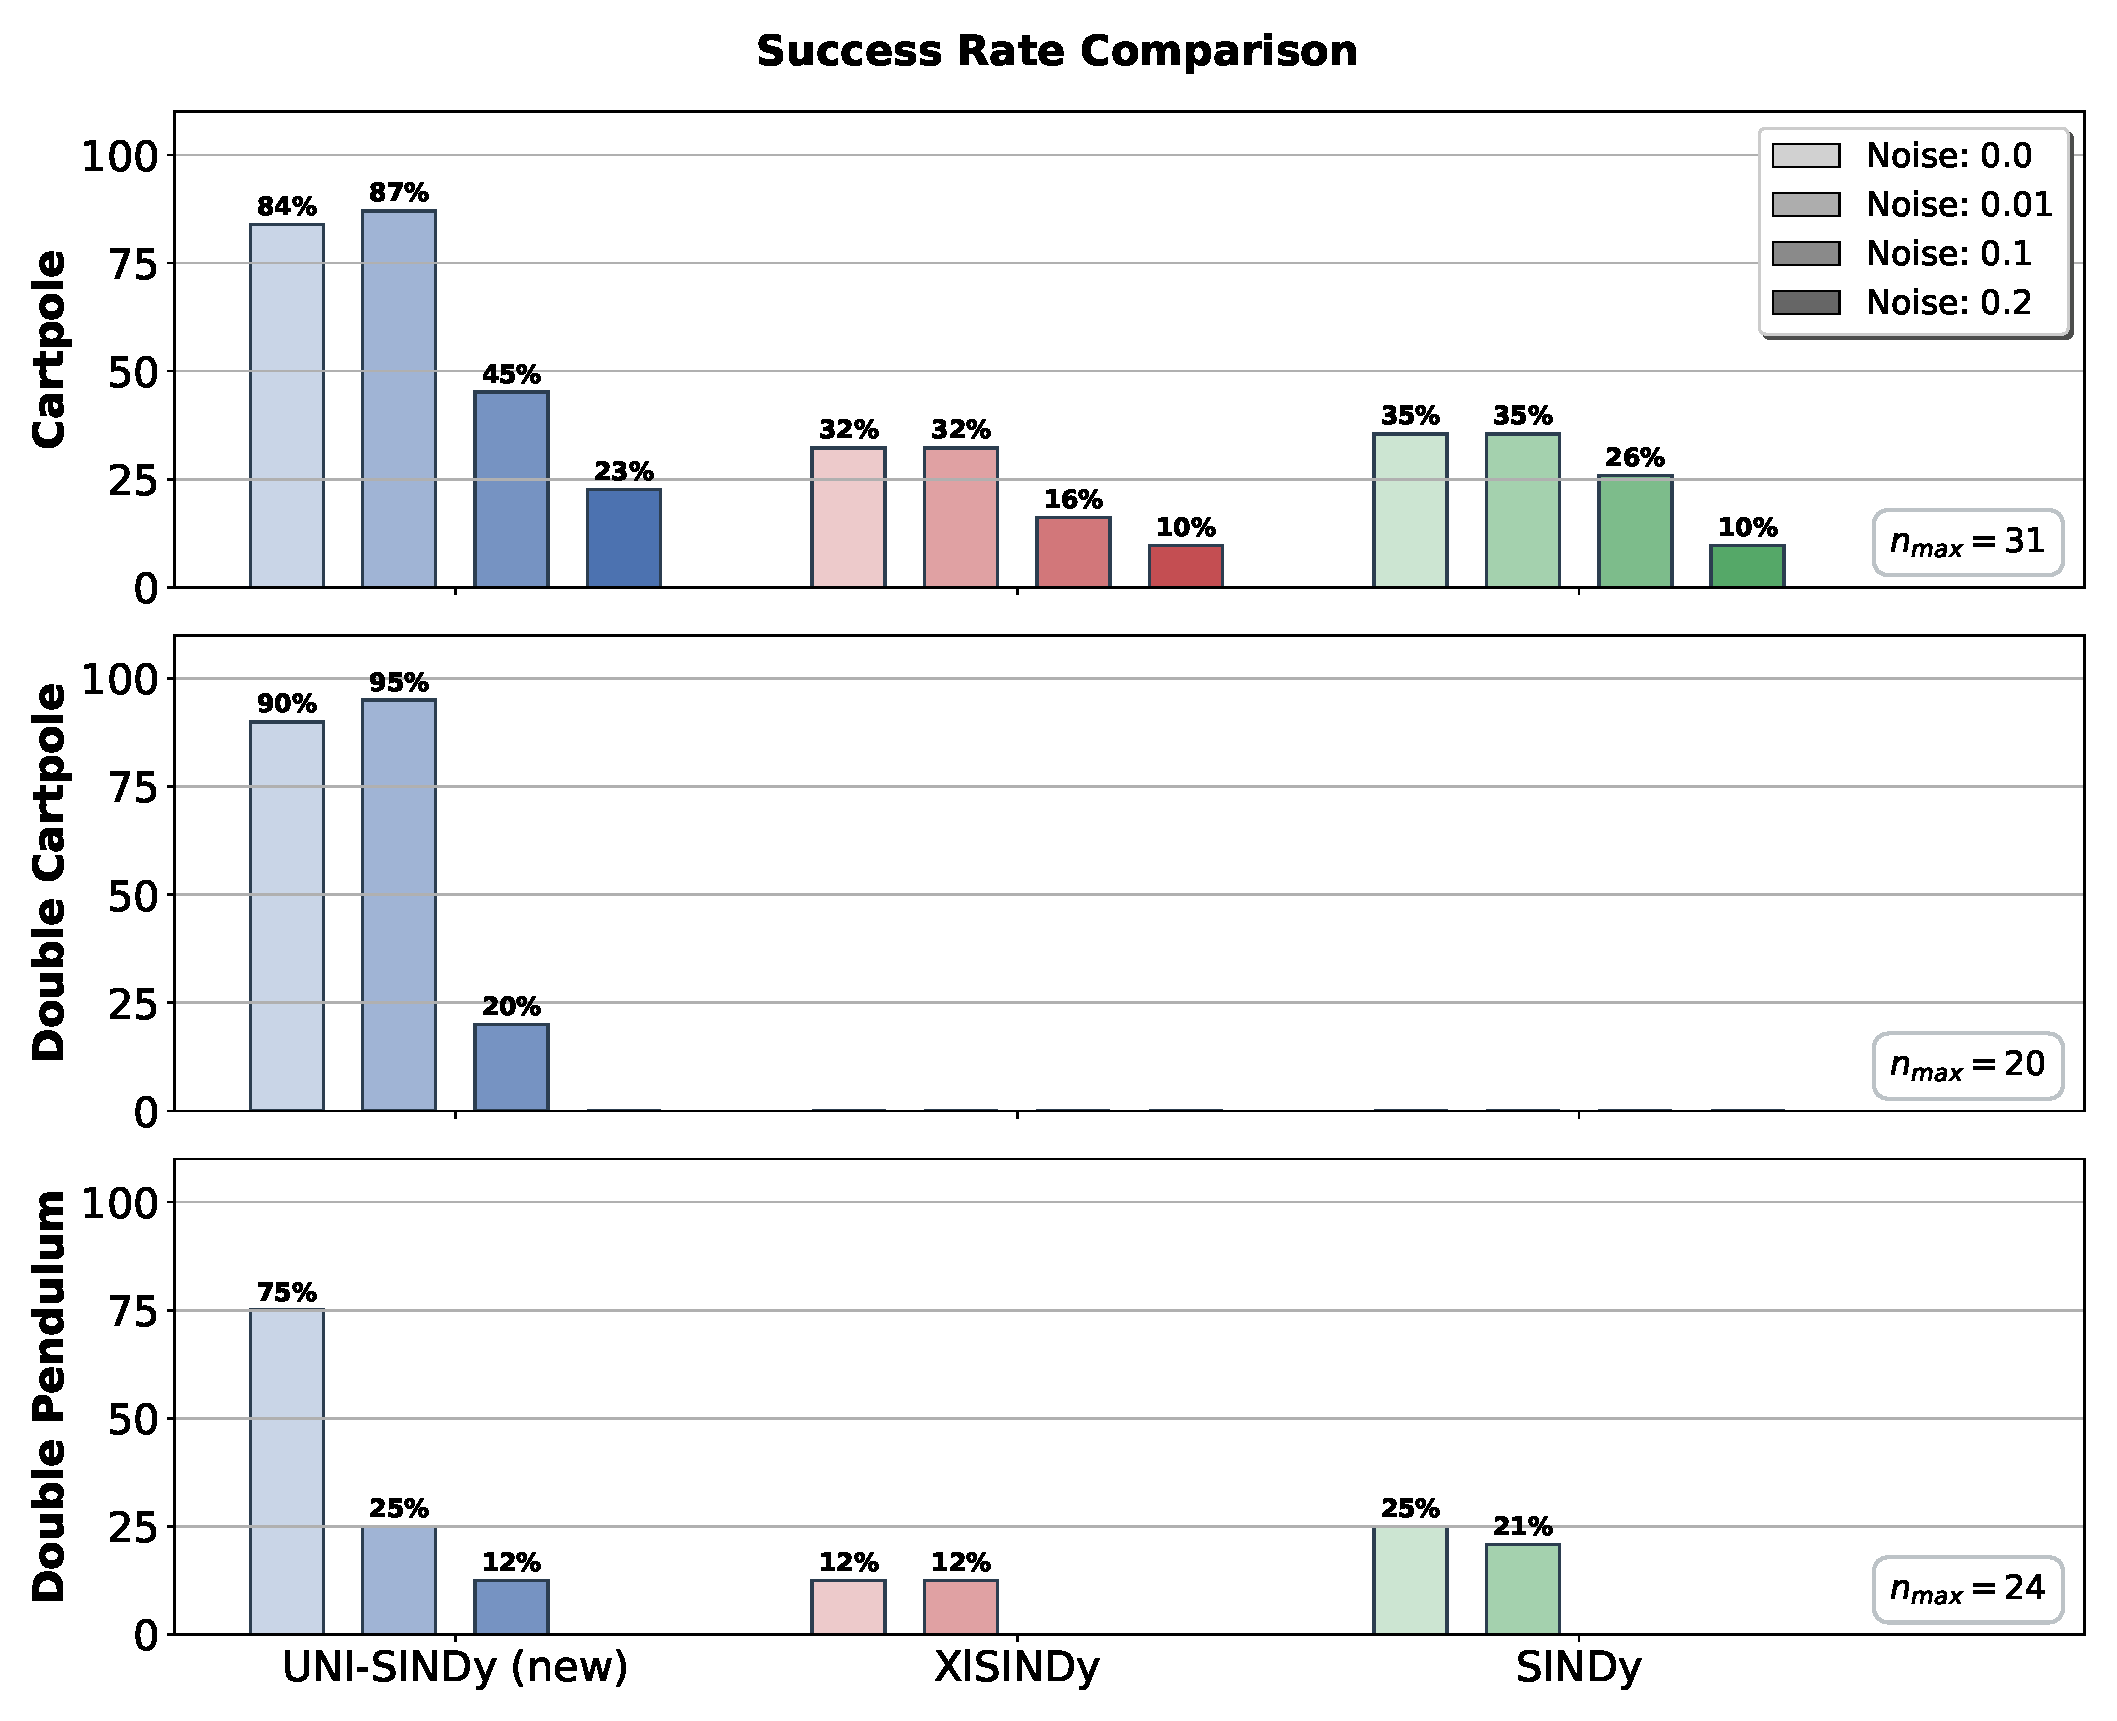
\includegraphics[width=\textwidth]{result/plots_damping_mixed/success_rate_white_background.eps}
        \caption{Success rate}
    \end{subfigure}
    
    \vspace{0.5cm}
    
    \begin{subfigure}[b]{0.95\textwidth}
        \includegraphics[width=\textwidth]{result/plots_damping_mixed/success_rate_combined_white_background.eps}
        \caption{Success rate combined}
    \end{subfigure}
    \caption{Damping mixed - Success rate comparison}
    \label{fig:damping_mixed_success}
\end{figure}

\section{No Damping Explicit Results}

\begin{figure}[H]
    \centering
    \begin{subfigure}[b]{0.95\textwidth}
        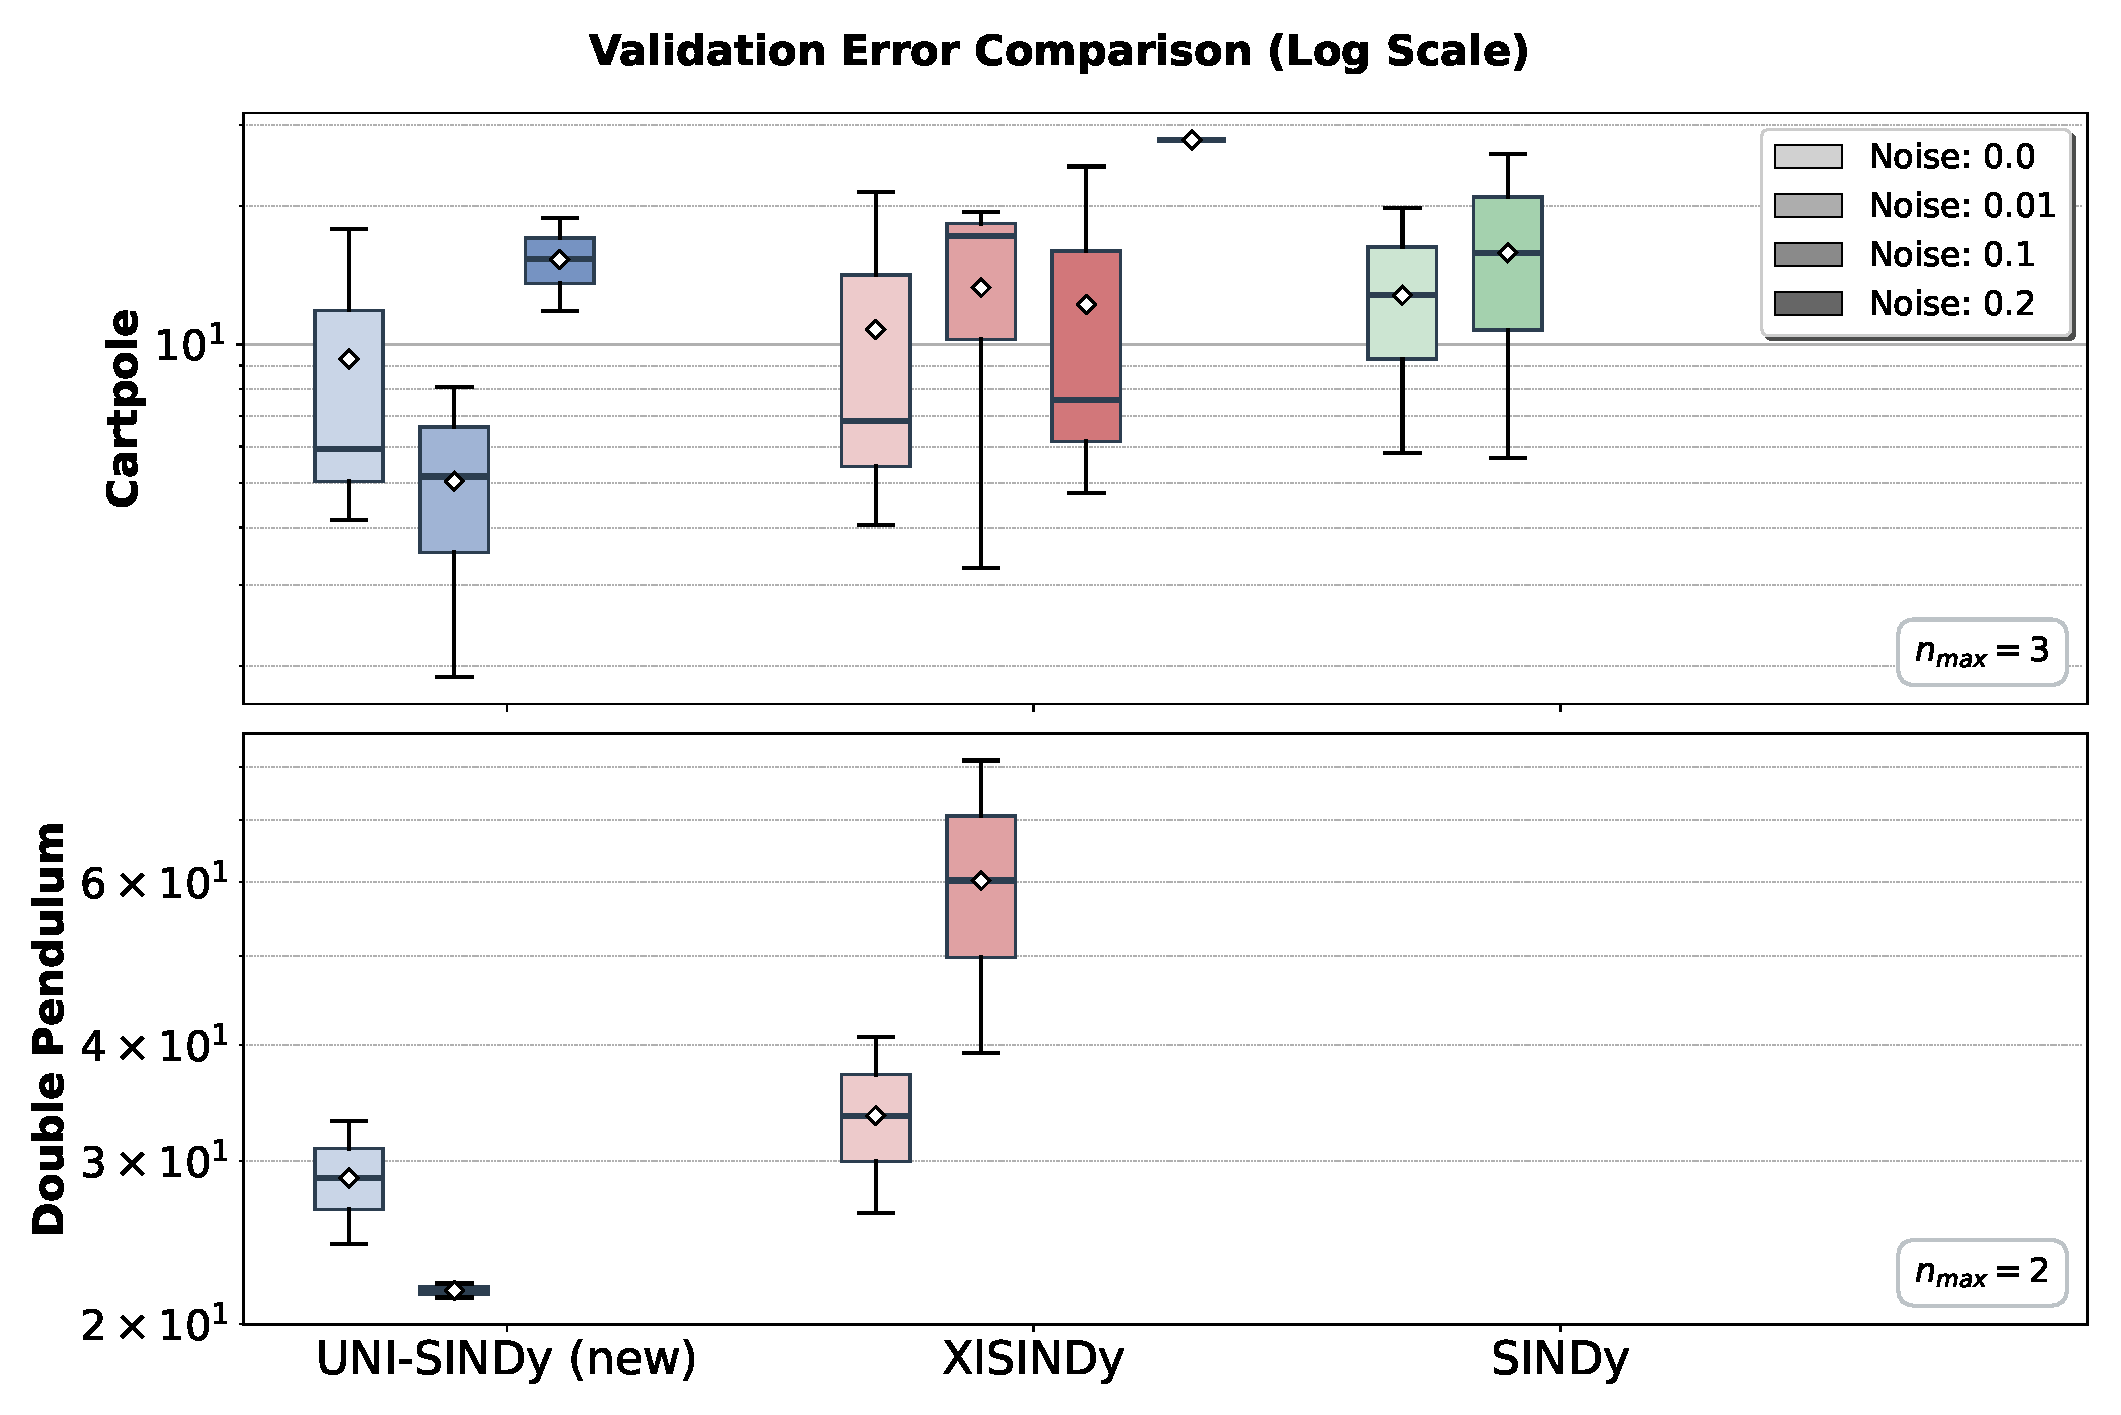
\includegraphics[width=\textwidth]{result/plots_no_damping_explicit/noise_comparison_white_background.eps}
        \caption{Noise comparison}
    \end{subfigure}
    
    \vspace{0.5cm}
    
    \begin{subfigure}[b]{0.95\textwidth}
        \includegraphics[width=\textwidth]{result/plots_no_damping_explicit/noise_comparison_combined_white_background.eps}
        \caption{Noise comparison combined}
    \end{subfigure}
    \caption{No damping explicit - Validation error comparison}
    \label{fig:no_damping_explicit_validation}
\end{figure}

\begin{figure}[H]
    \centering
    \begin{subfigure}[b]{0.95\textwidth}
        \includegraphics[width=\textwidth]{result/plots_no_damping_explicit/success_rate_white_background.eps}
        \caption{Success rate}
    \end{subfigure}
    
    \vspace{0.5cm}
    
    \begin{subfigure}[b]{0.95\textwidth}
        \includegraphics[width=\textwidth]{result/plots_no_damping_explicit/success_rate_combined_white_background.eps}
        \caption{Success rate combined}
    \end{subfigure}
    \caption{No damping explicit - Success rate comparison}
    \label{fig:no_damping_explicit_success}
\end{figure}

\end{document}